\documentclass{article}
\usepackage[utf8]{inputenc}
\usepackage[english]{babel}
\usepackage{titling}
\usepackage{xcolor}
\usepackage{amsmath}
\usepackage{hyperref}
\usepackage{listings}
\usepackage[T1]{fontenc}
\usepackage{underscore}
\usepackage{natbib}
\usepackage{graphicx}
\usepackage{color}
\usepackage{listings}
\usepackage{graphicx}
\usepackage{amssymb}
\usepackage[rightcaption]{sidecap}
\usepackage{subcaption}
\usepackage{wrapfig}
\usepackage{tcolorbox}
\usepackage{tabularx}
\usepackage{filecontents}
\usepackage{standalone}
\usepackage{float}
\usepackage{blindtext}
\usepackage{imakeidx}
\usepackage[margin=1.6in]{geometry}
\usepackage{fancyhdr}
\usepackage{tikz}
\usepackage{titling}
\usepackage{caption}
\usepackage{bbding}
\usepackage{pxfonts}

\usetikzlibrary{positioning, arrows, automata, chains, shapes, positioning}
\usetikzlibrary{decorations.pathreplacing}

\definecolor{myLightGray}{RGB}{191,191,191}
\definecolor{myGray}{RGB}{160,160,160}
\definecolor{myDarkGray}{RGB}{144,144,144}
\definecolor{myMoreDarkRed}{RGB}{100,100,100}
\definecolor{myDeepGray}{RGB}{50,50,50}
\definecolor{myGreen}{RGB}{0,255,71}

\setcounter{tocdepth}{4}
\setcounter{secnumdepth}{5}
\definecolor{lstgrey}{rgb}{0.95,0.95,0.95}
\lstset{language=C, backgroundcolor=\color{lstgrey}, frame=single, basicstyle=\footnotesize\ttfamily, captionpos=b, tabsize=2}


\makeindex
\title{
\large{Quick user manual}
}

\makeatletter
\let\oldtitle\@title
\def\@title{
\includegraphics[scale=0.5]{fig/quarkts.png}\\\oldtitle}
\makeatother

%\title{User Manual \\ \small{valid for v4.9.1}}
%\title{
\includegraphics[scale=0.2]{fig/quarkts.png}\\ Brief Article}

\author{J. Camilo Gómez C.}
\date{\today}

\pagestyle{fancy}
\fancyhf{}
\lhead{
\includegraphics[scale=0.2]{fig/quarkts.png}}
\rhead{Quick user manual for v6.2}
\renewcommand{\headrulewidth}{2pt}
\renewcommand{\footrulewidth}{1pt}
\rfoot{Page \thepage}

\definecolor{mGreen}{rgb}{0,0.6,0}
\definecolor{mGray}{rgb}{0.5,0.5,0.5}
\definecolor{mPurple}{rgb}{0.58,0,0.82}
\definecolor{mBlue}{rgb}{0,0.3,0.68}
\definecolor{mBlue2}{rgb}{0,0.35,0.17}
\definecolor{backgroundColour}{rgb}{0.95,0.95,0.95}

\lstdefinestyle{CStyle}{
    backgroundcolor=\color{backgroundColour},   
    commentstyle=\color{gray},
    keywordstyle=\color{blue},
    numberstyle=\tiny\color{mGray},
    stringstyle=\color{mPurple},
    basicstyle=\ttfamily\footnotesize,
    breakatwhitespace=false,         
    breaklines=true,                 
    captionpos=b,                    
    keepspaces=true,                 
    showspaces=false,                
    showstringspaces=false,
    showtabs=false,                  
    tabsize=2,
    language=C,
    classoffset = 1,
    morekeywords = {qBool_t, qTask_t, qPriority_t, qIteration_t, qState_t, qTime_t, qGetTickFcn_t, qTimingBase_t, qTaskFcn_t, qEvent_t, qCR_Begin, qCR_End, qCR_Yield, qUINT8_t, qUINT16_t, qUINT32_t, size_t, qINT8_t, qINT16_t, qINT32_t, qFloat32_t, qFloat64_t, qTask_GlobalState_t, qTaskFlag_t, qTrigger_t, qQueue_t, qQueue_LinkMode_t, qSTimer_t, qClock_t, qSM_t, qSM_Status_t, qSM_Handler_t, qSM_State_t, qSM_SubState_t, qSM_Attribute_t, qSM_TransitionTable_t, qSM_Transition_t, qSM_Signal_t, qCR_Delay, qCR_WaitUntil, qCR_Do, qCR_Until, qCR_PositionGet, qCR_PositionRestore, qCR_PositionReset, qCR_SemInit, qCR_SemWait, qCR_SemSignal, qCR_Semaphore_t, qATCLI_t, qPutChar_t, qATCLI_Command_t, qATCLI_CommandCallback_t, qATCLI_Options_t, qATCLI_Response_t, qATCLI_PreCmd_t, qATCLI_Handler_t, qMemMang_Pool_t, qTrace_Var, qTrace_Variable, qDebug_Var, qDebug_Variable, qTrace, qDebug, qTrace_Mem, qTrace_Memory, qBSBuffer_t, qEdgeCheck_t, qCoreRegSize_t, qEdgeCheck_IONode_t, qList_t, qList_Position_t, qList_Direction_t, qList_NodeFcn_t, qList_Iterator_t, qResponse_t, qGetChar_t, qTask_NotifyMode_t, qCycles_t},    
    keywordstyle=\color{mBlue},
    classoffset = 2,
    morekeywords = { qPeriodic, qEnabled, qHigh_Priority, qMedium_Priority, qLowest_Priority, qTimeImmediate, qTrue, qFalse, QEVENTFLAG_01, QEVENTFLAG_02, QEVENTFLAG_03, QEVENTFLAG_04, QEVENTFLAG_SET, NULL, qQUEUE_EMPTY, qQUEUE_COUNT, qATTACH, byQueueCount, byQueueEmpty, byNotificationSimple, byNotificationQueued, byTimeElapsed, QSTIMER_INITIALIZER, qSM_EXIT_SUCCESS, qSM_EXIT_FAILURE, QSM_SIGNAL_ENTRY, QSM_SIGNAL_EXIT, QATCLI_NORESPONSE, QATCLI_OK, QATCLI_CMDTYPE_PARA, QATCLI_CMDTYPE_ACT, QATCLI_CMDTYPE_TEST, QATCLI_CMDTYPE_READ, QATCLI_ERROR, qNode_MinimalFields},    
    keywordstyle=\color{mBlue2},    
    classoffset =3,
    morekeywords = {qOS_Setup, qClock_SysTick, qOS_Set_IdleTask, qOS_Add_Task, qOS_Add_EventTask, qOS_Remove_Task, qOS_Run, qOS_Set_SchedulerReleaseCallback, qCritical_SetInterruptsED, qTask_Set_Time, qTask_Set_Iterations, qTask_Set_Priority, qTask_Set_Callback, qTask_Set_State, qTask_Resume, qTask_Suspend, qTask_ASpeep, qTask_Awake, qTask_Set_Data, qTask_ClearTimeElapsed, qTask_Get_Cycles, qTask_Get_State, qTask_Self, qTask_Get_GlobalState, qTask_HasPendingNotifications, qTask_Notification_Send, qTask_Notification_Queue, qOS_Notification_Spread, qTask_EventFlags_Modify, qTask_EventFlags_Read, qTask_EventFlags_Check, qQueue_Setup, qQueue_SendToBack, qQueue_SendToFront, qQueue_Receive, qTask_Attach_Queue, qQueue_Reset, qQueue_IsEmpty, qQueue_Count, , qQueue_IsFull, qQueue_Peek, qQueue_RemoveFront, qSTimer_Set, qSTimer_FreeRun, qSTimer_Disarm, qSTimer_Elapsed, qSTimer_Remaining, qSTimer_Expired, qSTimer_Status, qStateMachine_Setup, qStateMachine_Run, qOS_Add_StateMachineTask, qStateMachine_Attribute, qStateMachine_TransitionTableInstall, qStateMachine_SignalQueueSetup, qStateMachine_SendSignal, qOS_StateMachineTask_SigCon, qStateMachine_Set_CompositeState, qATCLI_Setup, qATCLI_CmdSubscribe, qATCLI_ISRHandler, qATCLI_ISRHandlerBlock, qATCLI_Raise, qATCLI_Exec, qATCLI_Run, qOS_Add_ATCLITask, qATCLI_GetArgString, qATCLI_GetArgPtr, qATCLI_GetArgInt, qATCLI_GetArgFlt, qATCLI_GetArgHex, qMemMang_Pool_Select, qMenMang_Get_FreeSize, qMalloc, qFree, qTrace_Set_OutputFcn, qMemMang_Pool_Setup},
    keywordstyle=\bfseries,
    classoffset = 0,
}





\begin{document}


\maketitle

\tableofcontents

\clearpage
\newpage

\section{Background}
\subsection{About the OS}
QuarkTS is an open-source operating system that is built on top of a cooperative quasi-static scheduler. Its simplified kernel implements a specialized round-robin scheme using a linked-chain approach and an event-queue to provide true FIFO priority-scheduling.

Rather than having preemption,  tasks manage their own life-cycle. This bring significant benefits, fewer re-entrance problems are encountered, because tasks cannot be interrupted arbitrarily by other tasks, but only at positions permitted by the programmer. In addition with a state-machines support, co-routines, time control and the inter-task communication primitives, QuarkTS provides a modern environment to build stable and predictable event-driven multitasking embedded software.

These features make it suitable for resource-constrained microcontrollers, where a full-preemptive RTOS is an overkill and their inclusion adds unnecessary complexity to the firmware development. Their modularity and reliability make this OS a great choice to develop efficiently a wide range of applications in low-cost devices, including automotive controls, monitoring and Internet of Things.

\subsubsection{License}
QuarkTS is licensed under the GNU General Public License v3.0 (GPL-3). You may copy, distribute and modify the software as long as you track changes/dates in source files. Any modifications to this OS, including GPL-licensed code must also be made available under the GPL along with build \& install instructions. This OS is distributed in the hope that it will be useful, but WITHOUT ANY WARRANTY; without even the implied warranty of MERCHANTABILITY or FITNESS FOR A PARTICULAR PURPOSE. 
For more details, see the GNU General Public License for more details in \cite{license}. 

\subsubsection{Hardware compatibility}
QuarkTS has no direct hardware dependencies, so it is portable to many platforms and C compilers. 
The following cores have been powered with QuarkTS successfully:
\begin{itemize}
    \item ARM cores(ATMEL, STM32, LPC, Kinetis, Nordic and others)
    \item 8Bit AVR, 8051, STM8
    \item HCS12, ColdFire, MSP430
    \item PIC (PIC24, dsPIC, 32MX, 32MZ)
\end{itemize}

\subsubsection{Coding standard and naming convention}

\begin{itemize}
    \item All the QuarkTS implementation follows the C99 standard.
    \item The core source files try to conform most of the MISRA C 2004/2012 coding standard guidelines, allowing the OS to be used in safe-critical embedded systems. 
    \item In line with MISRA guides, unqualified standard \lstinline{char} and \lstinline{char *} types are only permitted to hold ASCII characters and strings respectively.
    \item In line with MISRA guides and for portability between platforms, we use the \lstinline{stdint.h} with typedefs that indicate size and signedness in place of the basic types.
    \item The \lstinline{_t} suffix its used to denote a type definition (i.e \lstinline{qBool_t, qTask_t, size_t, ...}).   
    \item Functions, macros, \lstinline{enum} values and data-types are prefixed \lstinline{q}. (i.e. \lstinline{qFunction}, \lstinline{qEnumValue}, \lstinline{QCONSTANT}, \lstinline{qType_t}, ...)
    \item Other than the pre-fix, most macros used for constants are written in all upper case.
    \item Almost all functions returns a boolean value of type \lstinline{qBool_t}, where a \lstinline{qTrue - 1u}  value indicates a successful procedure and \lstinline{qFalse - 0u}, the failure of the procedure.
\end{itemize}

\subsubsection{Memory usage}
As a quasi-static scheduler is implemented here, dynamic memory allocation is not required and the assignment of tasks must be done before program execution begins.
The kernel is designed to allow unlimited tasks and kernel objects, but of course, the whole application will be constrained by the memory specifications of the embedded system. \\
The kernel's memory footprint can be scaled down to contain only the features required for your application, typically 2.5 KBytes of code space and less than 1 KByte of data space. \\

\begin{tabular}{ |p{10cm}||p{1.5cm}|  }
 \hline
 \multicolumn{2}{|c|}{ \textbf{OS Memory Footprint} \scriptsize{(Measured in a 32bit MCU)}} \\
 \hline
 \textbf{Functionality} & \textbf{Size}\scriptsize{(bytes)}\\
 \hline
 Kernel, scheduler and task management& 2637\\
 A task node ({\lstinline!qTask_t!}) & 64\\
 Finite State-Machines(FSM) handling and related APIs& 314\\
 A FSM object ({\lstinline!qSM_t!}) & 37 \\
 STimers handling and related APIs & 258\\
 A STimer object ({\lstinline!qSTimer_t!})& 8\\
 qQueues handling and related APIS & 544\\
 A qQueue object ({\lstinline!qQueue_t!}) & 28\\
 Memory management & 407\\
 A memory pool ({\lstinline!qMemMang_Pool_t!}) & 28 \\ 
 The AT Command Parser & 1724\\
 An AT-Parser instance ({\lstinline!qATCLI_t!})& 112\\
 An AT command object ({\lstinline!qATCLI_Command_t!})& 24\\
 Remaining utilities& 2980\\
 \hline
\end{tabular}

 \begin{tcolorbox}
 \HandRight Although the kernel does not use dynamically-allocated resources internally, the application writer can create an object dynamically using the heap implementation provided by the memory management module described in section \ref{memmanagement}.
 \end{tcolorbox}

\subsection{Timing approach}
The kernel implements a Time-Triggered Architecture (TTA)\cite{pont}, in which the tasks are triggered by comparing the corresponding task-time with a reference clock. The reference clock must be real-time and follow a monotonic behavior. Usually, all embedded systems can provide this kind of reference with a constant tick generated by a periodic background hardware-timer, typically, at 1Khz (1mS tick). 

For this, the kernel allows you to select the reference clock source among these two scenarios:

\begin{itemize}
    \item  When tick already provided: The reference is supplied by the Hardware Abstraction Layer (HAL) of the device.
        It is the simplest scenario and it occurs when the framework or SDK of the embedded system includes a HAL-API that obtains the time elapsed since the system starts, usually in milliseconds and taking a  32-bit counter variable.
    \item When the tick is not provided: The application writer should use bare-metal code to configure the device and feed the reference clock manually.
        Here, a hardware timer should raise an interrupt periodically. After the \textit{Interrupt Service Routine} (ISR) has been implemented using the platform-dependent code, the \lstinline{qClock_SysTick()} \index{\lstinline{qClock_SysTick}} API must be called inside. It is recommended that the reserved ISR should only be used by QuarkTS.
\end{itemize}

\subsection{Setting up the OS kernel : \lstinline{qOS_Setup}} \label{settingupkernel}
 This function should be the first call to the OS APIs. \lstinline{qOS_Setup()} \index{\lstinline{qOS_Setup}} prepares the kernel instance, sets the reference clock, defines the \textit{Idle-Task} callback and allocates the stack for the internal queue. \\
 
\begin{lstlisting}[style=CStyle]
void qOS_Setup( const qGetTickFcn_t TickProvider, 
                const qTimingBase_t BaseTimming, 
                qTaskFcn_t IdleCallback )
\end{lstlisting}


\subsubsection*{Parameters}
\begin{itemize}
    \item \lstinline{TickProvider} : The function that provides the tick value. If the user application uses the \lstinline{qClock_SysTick()} from the ISR, this parameter can be \lstinline{NULL}. \\
    Note: Function should take \lstinline{void} and return a 32bit unsigned integer.  \\
    This argument must have this prototype : \lstinline{qUINT32_t TickProviderFcn(void)}
    \item \lstinline{BaseTimming} :This parameter specifies the ISR background timer period in seconds(floating-point format).
    
    \textit{Note} : This argument will be only available if \lstinline{Q_SETUP_TIME_CANONICAL} is set to zero(0).
    \item \lstinline{IdleCallback} : Callback function for the idle task. If not used, pass \lstinline{NULL} as argument.
\end{itemize}


\begin{tcolorbox}
\HandRight This call is mandatory and must be called once in the application main thread before any kind of interaction with the OS.
\end{tcolorbox}

\subsubsection*{Usage example:}
Scenario 1: When tick is already provided
\begin{lstlisting}[style=CStyle]
#include "QuarkTS.h"
#include "HAL.h"

#define TIMER_TICK   0.001   /* 1ms */ 

void main( void ){
    HAL_Init(); 
    qOS_Setup( HAL_GetTick, TIMER_TICK, IdleTask_Callback );
    
    /*
    TODO: add Tasks to the scheduler scheme and run the OS
    */
}
\end{lstlisting}


Scenario 2: When the tick is not provided
\begin{lstlisting}[style=CStyle]
#include "QuarkTS.h"
#include "DeviceHeader.h"

#define TIMER_TICK   0.001   /* 1ms */ 

void Interrupt_Timer0( void ){
    qClock_SysTick();
}

void main( void ){
    MCU_Init();
    BSP_Setup_Timer0(); 
    qOS_Setup( NULL, TIMER_TICK, IdleTask_Callback ); 
    
    /*
    TODO: add Tasks to the scheduler scheme and run the OS
    */
}
\end{lstlisting}

\subsection{Tasks}
Like many operating systems, the basic unit of work is the task. Tasks can perform certain functions, which could require periodic or one-time execution, update of specific variables or waiting for specific events. Tasks also could be controlling specific hardware or be triggered by hardware interrupts. In the QuarkTS OS, a task is seen as a node concept that links together:

\begin{itemize}
    \item Program code performing specific task activities (callback function)
    \item Execution interval (time)
    \item Number of execution (iterations)
    \item Event-based data
\end{itemize}

The OS  uses a \textit{Task Control Block} (TCB) to represent each task, storing essential information about task management and execution. Part of this information also includes \textit{link-pointers} that allows it to be part of one of the lists available in the Kernel Control Block (KCB).

\begin{figure}[H]
    \centering
    \tikzset{every picture/.style={line width=0.75pt}} %set default line width to 0.75pt        
    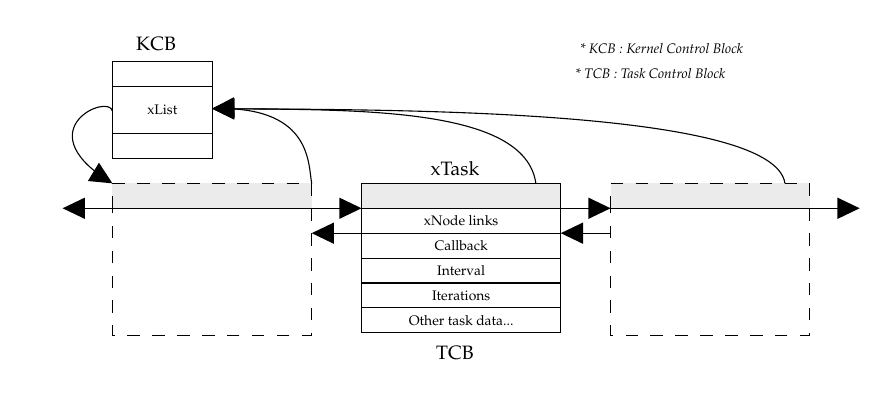
\begin{tikzpicture}[x=0.75pt,y=0.75pt,yscale=-1,xscale=1,scale=1.2]
        \draw   (220,99) -- (300,99) -- (300,109) -- (220,109) -- cycle ;
        \draw  [fill=lightgray!50  ,fill opacity=0.62 ] (220,79) -- (300,79) -- (300,89) -- (220,89) -- cycle ;
        \draw    (220,99) -- (203,99) ;
        \draw [shift={(200,99)}, rotate = 360] [fill=black][line width=0.08]  [draw opacity=0] (8.93,-4.29) -- (0,0) -- (8.93,4.29) -- cycle;
        \draw   (220,109) -- (300,109) -- (300,119) -- (220,119) -- cycle ;
        \draw   (220,119) -- (300,119) -- (300,129) -- (220,129) -- cycle ;
        \draw  [dash pattern={on 4.5pt off 4.5pt}] (320,89) -- (400,89) -- (400,140) -- (320,140) -- cycle ;
        \draw  [fill=lightgray!50  ,fill opacity=0.62 ][dash pattern={on 4.5pt off 4.5pt}] (320,79) -- (400,79) -- (400,89) -- (320,89) -- cycle ;
        \draw   (220,129) -- (300,129) -- (300,139) -- (220,139) -- cycle ;
        \draw  [dash pattern={on 4.5pt off 4.5pt}] (120,89) -- (200,89) -- (200,140) -- (120,140) -- cycle ;
        \draw  [fill=lightgray!50  ,fill opacity=0.62 ][dash pattern={on 4.5pt off 4.5pt}] (120,79) -- (200,79) -- (200,89) -- (120,89) -- cycle ;
        \draw    (200,89) -- (217,89) ;
        \draw [shift={(220,89)}, rotate = 180] [fill=black][line width=0.08]  [draw opacity=0] (8.93,-4.29) -- (0,0) -- (8.93,4.29) -- cycle;
        \draw   (220,89) -- (300,89) -- (300,99) -- (220,99) -- cycle ;
        \draw    (320,99) -- (303,99) ;
        \draw [shift={(300,99)}, rotate = 360] [fill=black][line width=0.08]  [draw opacity=0] (8.93,-4.29) -- (0,0) -- (8.93,4.29) -- cycle;
        \draw    (300,89) -- (317,89) ;
        \draw [shift={(320,89)}, rotate = 180] [fill=black][line width=0.08]  [draw opacity=0] (8.93,-4.29) -- (0,0) -- (8.93,4.29) -- cycle;
        \draw    (120,89) -- (103,89) ;
        \draw [shift={(100,89)}, rotate = 360] [fill=black][line width=0.08]  [draw opacity=0] (8.93,-4.29) -- (0,0) -- (8.93,4.29) -- cycle;
        \draw    (400,89) -- (417,89) ;
        \draw [shift={(420,89)}, rotate = 180] [fill=black][line width=0.08]  [draw opacity=0] (8.93,-4.29) -- (0,0) -- (8.93,4.29) -- cycle;
        \draw   (120,30) -- (160,30) -- (160,40) -- (120,40) -- cycle ;
        \draw   (120,40) -- (160,40) -- (160,59) -- (120,59) -- cycle ;
        \draw   (120,59) -- (160,59) -- (160,69) -- (120,69) -- cycle ;
        \draw    (290,79) .. controls (285.57,48.04) and (217.59,49.52) .. (162.51,49.02) ;
        \draw [shift={(160,49)}, rotate = 360.59] [fill=black][line width=0.08]  [draw opacity=0] (8.93,-4.29) -- (0,0) -- (8.93,4.29) -- cycle;
        \draw    (200,79) .. controls (198.54,71.76) and (200.4,48.76) .. (162.96,48.94) ;
        \draw [shift={(160,49)}, rotate = 357.98] [fill=black][line width=0.08]  [draw opacity=0] (8.93,-4.29) -- (0,0) -- (8.93,4.29) -- cycle;
        \draw    (390,79) .. controls (385.57,48.04) and (220.56,49.52) .. (162.57,49.02) ;
        \draw [shift={(160,49)}, rotate = 360.59] [fill=black][line width=0.08]  [draw opacity=0] (8.93,-4.29) -- (0,0) -- (8.93,4.29) -- cycle;
        \draw    (120,50) .. controls (118.54,42.76) and (86.18,56.84) .. (117.47,77.41) ;
        \draw [shift={(120,79)}, rotate = 211.12] [fill=black][line width=0.08]  [draw opacity=0] (8.93,-4.29) -- (0,0) -- (8.93,4.29) -- cycle;
        \draw (260,104) node  [font=\tiny] [align=left] {Callback};
        \draw (260,114) node  [font=\tiny] [align=left] {Interval};
        \draw (260,124) node  [font=\tiny] [align=left] {Iterations};
        \draw (260,134) node  [font=\tiny] [align=left] {Other task data...};
        \draw (257.5,147) node  [font=\scriptsize] [align=left] {TCB};
        \draw (260,94) node  [font=\tiny] [align=left] {xNode links};
        \draw (137.5,23) node  [font=\scriptsize] [align=left] {KCB};
        \draw (140,49.5) node  [font=\tiny] [align=left] {xList};
        \draw (257.5,73) node  [font=\scriptsize] [align=left] {xTask};
        \draw (340.5,25) node  [font=\tiny] [align=left] {\textit{* KCB : Kernel Control Block}};
        \draw (336,35) node  [font=\tiny] [align=left] {\textit{* TCB : Task Control Block}};
    \end{tikzpicture}
\caption{Task node illustration}
\label{fig:tasklist}
\end{figure}

Each task performs its activities via a callback function and each of them is responsible for supporting cooperative multitasking by being “good neighbors”, i.e., running their callback methods quickly in a non-blocking way and releasing control back to the scheduler as soon as possible (returning). \\

Every task node, must be defined using the \lstinline{qTask_t} \index{\lstinline{qTask_t}} data-type and the callback is defined as a function that returns \lstinline{void} and takes a \lstinline{qEvent_t} data structure as its only parameter (This input argument can be used later to get event information, see section \ref{eventdata}).

\begin{lstlisting}[style=CStyle]
qTask_t UserTask;
void UserTask_Callback( qEvent_t eventdata ){
    /* TODO : Task code */
}
\end{lstlisting}

\begin{tcolorbox}
\ArrowBoldDownRight \textit{Note} : All tasks in QuarkTS must ensure their completion to return the CPU control back to the scheduler, otherwise, the scheduler will hold the execution-state for that task, preventing the activation of other tasks.
\end{tcolorbox}

\subsubsection{The idle task}
Its a special task loaded by the OS scheduler when there is nothing else to do (no task in the whole scheme has reached the ready state). The idle task is already hard-coded into the kernel, ensuring that at least, one task is able to run. Additionally, the OS setup this task with the lowest possible priority to ensure that does not use any CPU time if there are higher priority application tasks able to run. \\
The idle task doesn't perform any active functions, but the user can decide if it should perform some activities defining a callback function for it. This could be done at the beginning of the kernel setup (as seen in section \ref{settingupkernel} with \lstinline{qOS_Setup()}) or in run-time with \lstinline{qOS_Set_IdleTask()} \index{\lstinline{qOS_Set_IdleTask}}. \\

\begin{lstlisting}[style=CStyle]
void qOS_Set_IdleTask(qTaskFcn_t Callback)
\end{lstlisting}

Of course, the callback must follow the same function prototype for tasks. \\

\begin{tcolorbox}
\HandRight To disable the idle-task activities, a \lstinline{NULL} should be passed as argument.
\end{tcolorbox}

\subsubsection{Adding tasks to the scheme : \lstinline{qOS_Add_Task} } \label{addtask}
After setting up the kernel with \lstinline{qOS_Setup()}, the user can proceed to deploy the multitasking application by adding tasks. If the task node and their respective callback is already defined, the task can be added to the scheme using \lstinline{qOS_Add_Task()} \index{\lstinline{qOS_Add_Task}}. This API can schedule a task to run every \lstinline{Time} seconds, \lstinline{nExecutions} times and executing \lstinline{CallbackFcn} method on every pass.\\

\begin{lstlisting}[style=CStyle]
qBool_t qOS_Add_Task( qTask_t * const Task, qTaskFcn_t CallbackFcn, 
                      qPriority_t Priority, qTime_t Time, 
                      qIteration_t nExecutions, qState_t InitialState, 
                      void* arg )
\end{lstlisting}

\subsubsection*{Parameters}
\begin{itemize}
    \item \lstinline{Task} : A pointer to the task node. 
    \item \lstinline{CallbackFcn} : A pointer to a void callback method with a \lstinline{qEvent_t} parameter as input argument..
    \item \lstinline{Priority} : The priority value. [0(min) - \lstinline{Q_PRIORITY_LEVELS}(max)]
    \item \lstinline{Time} : Execution interval defined in seconds (floating-point format). For immediate execution use the  \lstinline{qTimeImmediate} definition. 
    \item \lstinline{nExecutions} : Number of task executions (Integer value). For indefinite execution  use \lstinline{qPeriodic} or the \lstinline{qIndefinite} definition. 
    \item \lstinline{InitialState} : Specifies the initial operational state of the task (\lstinline{qEnabled}, \lstinline{qDisabled}, \lstinline{qAsleep} or \lstinline{qAwake}(implies \lstinline{qEnabled})).
    \item \lstinline{arg} - Represents the task argument. This argument must be passed by reference and cast to \lstinline{(void *)}. 
\end{itemize}

\subsubsection*{Return value}
\lstinline{qTrue} if the task was successfully added the scheme. Otherwise returns \lstinline{qFalse}.

\subsubsection*{Caveats}
\begin{enumerate}
    \item A task with \lstinline{Time} argument defined in \lstinline{qTimeImmediate}, will always get the \textit{qReady} state in every scheduling cycle, as consequence, the idle task will never gets dispatched.
    \item Tasks do not remember the number of iteration set initially by the \lstinline{nExecutions} argument. After the iterations are done, the internal iteration counter decreases until reach the zero. If another set of iterations is needed, the user should set the number of iterations again and resume the task explicitly. 
    \item Tasks that performed all their iterations, put their own state to \lstinline{qDisabled}. Asynchronous triggers do not affect the iteration counter.
    \item The \lstinline{arg} parameter can be used as storage pointer, so, for multiple data, create a structure with the required members and pass a pointer to that structure.
\end{enumerate}

\noindent\hrulefill

Invoking \lstinline{qOS_Add_Task()}  is the most generic way to adding tasks to the scheme, supporting a mixture of time-triggered and event-triggered tasks, however, additional simplified API functions are also provided to add specific purpose tasks:
\begin{itemize}
    \item Event-triggered only tasks $\rightarrow$ \lstinline{qOS_Add_EventTask()}
    \item State-machine tasks $\rightarrow$ \lstinline{qOS_Add_StateMachineTask()}. See section \ref{statemachinetask}.
    \item AT Command Line Interface tasks $\rightarrow$ \lstinline{qOS_Add_ATCLITask()}. See section \ref{runningparser}.
\end{itemize}


\subsubsection{Event-triggered tasks}
An event-triggered task reacts asynchronously to the occurrence of events in the system, such as external interrupts or changes in the available resources. 

The API \lstinline{qOS_Add_EventTask()} \index{\lstinline{qOS_Add_EventTask}} is intended to add this kind of tasks, keeping it in a \textit{qSuspended} state. Only asynchronous events followed by their priority value dictates when a task can change to the \textit{qRunning} state. \\


\begin{lstlisting}[style=CStyle]
qBool_t qOS_Add_EventTask( qTask_t * const Task, qTaskFcn_t CallbackFcn, 
                           qPriority_t Priority, void* arg)
\end{lstlisting}

As seen above, arguments related to timing and iterations parameters are dispensed and the only required arguments become minimal, just needing:  \lstinline{CallbackFcn}, \lstinline{Priority} and the related task arguments \lstinline{arg}.

\subsubsection{Removing a task : \lstinline{qOS_Remove_Task}}
As expected, the API \index{\lstinline{qOS_Remove_Task}}removes the task from the scheduling scheme.  This means the task node will be disconnected from the kernel chain, preventing additional overhead provided by the scheduler when it does checks over it and course, preventing from running. \\

\begin{lstlisting}[style=CStyle]
qBool_t qOS_Remove_Task( qTask_t * const Task )
\end{lstlisting}

\subsubsection*{Caveats:}
Task nodes are variables like any other. They allow your application code to reference a task, but there is no link back the other way and the kernel doesn't know anything about the variables, where the variable is allocated (stack, global, static, etc.) or how many copies of the variable you have made, or even if the variable still exists.  So the \lstinline{qOS_Remove_Task()} API cannot automatically free the resources allocated by the variable. 
If the task node has been dynamically allocated, the application writer it's responsible to free the memory block after a removal call.


\subsection{Running the OS : \lstinline{qOS_Run}}
After preparing the multitasking environment for your application, a call to \lstinline{qOS_Run()} \index{\lstinline{qOS_Run}} is required to execute the scheduling scheme.
This function is responsible to run the following OS main components:
\begin{itemize}
    \item \textbf{The Scheduler} : Select the tasks to be submitted into the system and decide with of them are able to run.
    \item \textbf{The Dispatcher} : When the scheduler completes its job of selecting ready tasks, it is the dispatcher which takes that task to the running state. This procedure gives a task control over the CPU after it has been selected by the scheduler. This involves the following:
    \begin{itemize}
        \item Preparing the resources before the task execution
        \item Execute the task activities (via the callback function)
        \item Releasing the resources after the task execution 
    \end{itemize}
\end{itemize}

The states involved in the interaction between the scheduler and dispatcher are described in the section that follows. \\

\begin{tcolorbox}
\ArrowBoldDownRight \textit{Note}: After calling \lstinline{qOS_Run()}, the OS scheduler will now be running, and the following line should never be reached, however, the user can optionally release it explicitly with \lstinline{qOS_Scheduler_Release()} API function.
\end{tcolorbox}

\subsubsection{Releasing the scheduler: \lstinline{qOS_Scheduler_Release} }
This functionality must be enabled from the \lstinline{Q_ALLOW_SCHEDULER_RELEASE} macro.
This API \index{\lstinline{qOS_Scheduler_Release}} stop the kernel scheduling. In consequence, the main thread will continue after the \lstinline{qOS_Run()} call. 

Although producing this action is not a typical desired behavior in any application, it can be used to handle a critical exception.

When used, the release will take place after the current scheduling cycle finish. The kernel can optionally include a release callback function that can be configured to get called if the scheduler is released. 
Defining the release callback,  will help to take actions over the exception that caused the release action. To enable this functionality, the \lstinline{qOS_Set_SchedulerReleaseCallback()} \index{\lstinline{qOS_Set_SchedulerReleaseCallback}} API should be used. \\

\begin{lstlisting}[style=CStyle]
void qOS_Set_SchedulerReleaseCallback( qTaskFcn_t Callback )
\end{lstlisting}

\begin{tcolorbox}
\HandRight When a scheduler release is performed, resources are not freed. After released, the application can invoke the \lstinline{qOS_Run()} again to resume the scheduling activities.
\end{tcolorbox}

\subsection{Global states and scheduling rules}

A task can be in one of the four global states: \textit{qRunning}, \textit{qReady}, \textit{qSuspended} or \textit{qWaiting}. Each of these states is tracked implicitly by putting the task in one of the associated kernel lists. 

These global states are described below:

\begin{figure}[H]
    \centering
    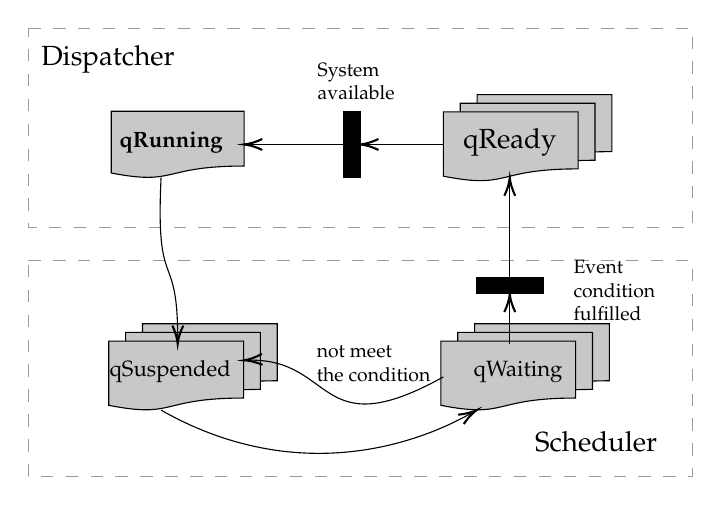
\begin{tikzpicture}[x=0.75pt,y=0.75pt,yscale=-1,xscale=1,scale=0.8]
        \draw  [fill={rgb, 255:red, 200; green, 200; blue, 200 }  ,fill opacity=1 ] (378.8,188) -- (460,188) -- (460,222.32) .. controls (409.25,222.32) and (419.4,234.7) .. (378.8,226.69) -- cycle ; \draw  [fill={rgb, 255:red, 200; green, 200; blue, 200 }  ,fill opacity=1 ] (368.65,193.2) -- (449.85,193.2) -- (449.85,227.52) .. controls (399.1,227.52) and (409.25,239.9) .. (368.65,231.89) -- cycle ; \draw  [fill={rgb, 255:red, 200; green, 200; blue, 200 }  ,fill opacity=1 ] (358.5,198.4) -- (439.7,198.4) -- (439.7,232.72) .. controls (388.95,232.72) and (399.1,245.1) .. (358.5,237.09) -- cycle ;
        \draw  [fill={rgb, 255:red, 200; green, 200; blue, 200 }  ,fill opacity=1 ] (178.8,188) -- (260,188) -- (260,222.32) .. controls (209.25,222.32) and (219.4,234.7) .. (178.8,226.69) -- cycle ; \draw  [fill={rgb, 255:red, 200; green, 200; blue, 200 }  ,fill opacity=1 ] (168.65,193.2) -- (249.85,193.2) -- (249.85,227.52) .. controls (199.1,227.52) and (209.25,239.9) .. (168.65,231.89) -- cycle ; \draw  [fill={rgb, 255:red, 200; green, 200; blue, 200 }  ,fill opacity=1 ] (158.5,198.4) -- (239.7,198.4) -- (239.7,232.72) .. controls (188.95,232.72) and (199.1,245.1) .. (158.5,237.09) -- cycle ;
        \draw  [fill={rgb, 255:red, 200; green, 200; blue, 200 }  ,fill opacity=1 ] (380.3,50) -- (461.5,50) -- (461.5,84.32) .. controls (410.75,84.32) and (420.9,96.7) .. (380.3,88.69) -- cycle ; \draw  [fill={rgb, 255:red, 200; green, 200; blue, 200 }  ,fill opacity=1 ] (370.15,55.2) -- (451.35,55.2) -- (451.35,89.52) .. controls (400.6,89.52) and (410.75,101.9) .. (370.15,93.89) -- cycle ; \draw  [fill={rgb, 255:red, 200; green, 200; blue, 200 }  ,fill opacity=1 ] (360,60.4) -- (441.2,60.4) -- (441.2,94.72) .. controls (390.45,94.72) and (400.6,107.1) .. (360,99.09) -- cycle ;
        \draw  [color={rgb, 255:red, 155; green, 155; blue, 155 }  ,draw opacity=1 ][dash pattern={on 4.5pt off 4.5pt}] (110,10) -- (510,10) -- (510,130) -- (110,130) -- cycle ;
        \draw  [fill={rgb, 255:red, 200; green, 200; blue, 200 }  ,fill opacity=1 ] (160,60) -- (240,60) -- (240,93) .. controls (190,93) and (200,104.9) .. (160,97.2) -- cycle ;
        \draw  [color={rgb, 255:red, 155; green, 155; blue, 155 }  ,draw opacity=1 ][dash pattern={on 4.5pt off 4.5pt}] (110,150) -- (510,150) -- (510,280) -- (110,280) -- cycle ;
        \draw    (360,220) .. controls (283.27,262.57) and (295.25,208.11) .. (241.64,209.93) ;
        \draw [shift={(240,210)}, rotate = 356.90999999999997] [color={rgb, 255:red, 0; green, 0; blue, 0 }  ][line width=0.75]    (10.93,-3.29) .. controls (6.95,-1.4) and (3.31,-0.3) .. (0,0) .. controls (3.31,0.3) and (6.95,1.4) .. (10.93,3.29);
        \draw    (190,240) .. controls (266.73,283.56) and (338.06,264.39) .. (378.78,240.72) ;
        \draw [shift={(380,240)}, rotate = 509.35] [color={rgb, 255:red, 0; green, 0; blue, 0 }  ][line width=0.75]    (10.93,-3.29) .. controls (6.95,-1.4) and (3.31,-0.3) .. (0,0) .. controls (3.31,0.3) and (6.95,1.4) .. (10.93,3.29)   ;
        \draw  [fill={rgb, 255:red, 0; green, 0; blue, 0 }  ,fill opacity=1 ] (420,160) -- (380,160) -- (380,170) -- (420,170) -- cycle ;
        \draw  [fill={rgb, 255:red, 0; green, 0; blue, 0 }  ,fill opacity=1 ] (310,60) -- (300,60) -- (300,100) -- (310,100) -- cycle ;
        \draw    (400,200) -- (400,172) ;
        \draw [shift={(400,170)}, rotate = 450] [color={rgb, 255:red, 0; green, 0; blue, 0 }  ][line width=0.75]    (10.93,-3.29) .. controls (6.95,-1.4) and (3.31,-0.3) .. (0,0) .. controls (3.31,0.3) and (6.95,1.4) .. (10.93,3.29)   ;
        \draw    (400,160) -- (400,102) ;
        \draw [shift={(400,100)}, rotate = 450] [color={rgb, 255:red, 0; green, 0; blue, 0 }  ][line width=0.75]    (10.93,-3.29) .. controls (6.95,-1.4) and (3.31,-0.3) .. (0,0) .. controls (3.31,0.3) and (6.95,1.4) .. (10.93,3.29)   ;
        \draw    (360,80) -- (312,80) ;
        \draw [shift={(310,80)}, rotate = 360] [color={rgb, 255:red, 0; green, 0; blue, 0 }  ][line width=0.75]    (10.93,-3.29) .. controls (6.95,-1.4) and (3.31,-0.3) .. (0,0) .. controls (3.31,0.3) and (6.95,1.4) .. (10.93,3.29)   ;
        \draw    (300,80) -- (242,80) ;
        \draw [shift={(240,80)}, rotate = 360] [color={rgb, 255:red, 0; green, 0; blue, 0 }  ][line width=0.75]    (10.93,-3.29) .. controls (6.95,-1.4) and (3.31,-0.3) .. (0,0) .. controls (3.31,0.3) and (6.95,1.4) .. (10.93,3.29)   ;
        \draw    (190,100) .. controls (186.54,172.27) and (200.22,140.65) .. (200.01,198.23) ;
        \draw [shift={(200,200)}, rotate = 270.48] [color={rgb, 255:red, 0; green, 0; blue, 0 }  ][line width=0.75]    (10.93,-3.29) .. controls (6.95,-1.4) and (3.31,-0.3) .. (0,0) .. controls (3.31,0.3) and (6.95,1.4) .. (10.93,3.29)   ;
        \draw (196,79) node  [scale=0.8, align=left] {\textbf{qRunning}};
        \draw (195.5,217) node [scale=0.8] [align=left] {qSuspended};
        \draw (405,217) node [scale=0.8] [align=left] {qWaiting};
        \draw (400,79) node [scale=1] [align=left] {qReady};
        \draw (158,29) node  [align=left] {Dispatcher};
        \draw (452,259) node  [align=left] {Scheduler};
        \draw (307.5,42) node [scale=0.7] [align=left] {System \\available};
        \draw (318,212) node [scale=0.7] [align=left] {not meet\\the condition};
        \draw (463,168) node [scale=0.7] [align=left] {Event\\condition\\fulfilled};
    \end{tikzpicture}
    \caption{Task global states}
    \label{fig:scheduler_states}
\end{figure}

\begin{itemize}
    \item \textbf{qWaiting} : The task cannot run because the conditions for running are not in place. 
    \item \textbf{qReady} : The task has completed preparations for running, but cannot run because a task with a higher precedence is running.
    \item \textbf{qRunning} : The task is currently being executed.
    \item \textbf{qSuspended} : The task doesn't take part in what is going on. Normally this state is taken after the \textit{qRunning} state or when the task doesn't reach the \textit{qReady} state.
\end{itemize}


The presence of a task in a particular list indicates the task's state. 
There are many ready-lists as defined in the \lstinline{Q_PRIORITY_LEVELS} macro.
To select the target ready list, the OS use the user-assigned priority between 0 (the lowest priority) and \lstinline{Q_PRIORITY_LEVELS-1} (the highest priority). For instance, if \lstinline{Q_PRIORITY_LEVELS} is set to 5, then QuarkTS will use 5 priority levels or ready lists: 0 (lowest priority), 1, 2, 3, and 4 (highest priority). 

\begin{figure}[H]
    \centering
    \tikzset{every picture/.style={line width=0.75pt}} %set default line width to 0.75pt        
    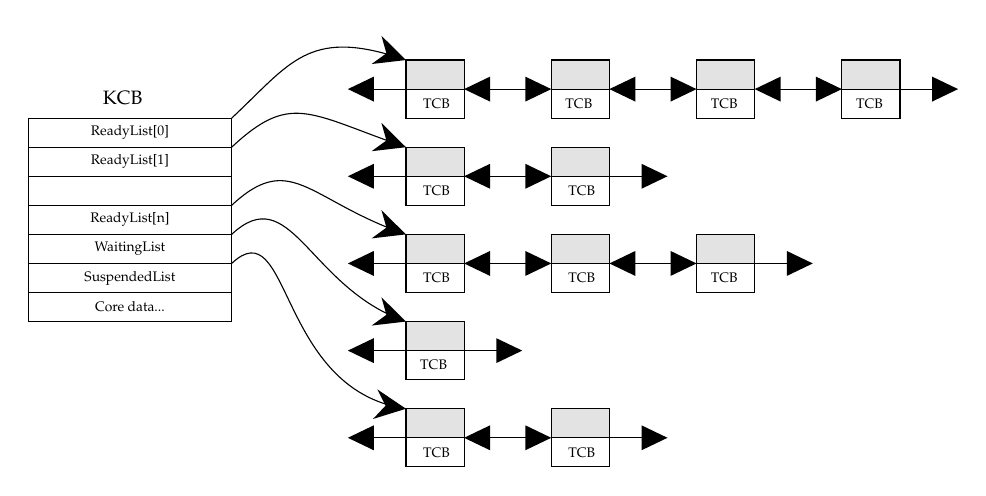
\begin{tikzpicture}[x=0.75pt,y=0.75pt,yscale=-1,xscale=1, scale=1.4]
        
        \foreach \x in {30,40,...,80}{
            \draw   (70,\x) -- (140,\x) -- (140,\x+10) -- (70,\x+10) -- cycle ;
        }
        
        \draw   (70,90) -- (140,90) -- (140,100) -- (70,100) -- cycle ;
        \draw   (200,10) -- (220,10) -- (220,30) -- (200,30) -- cycle ;
        \draw   (250,10) -- (270,10) -- (270,30) -- (250,30) -- cycle ;
        \draw  [fill={rgb, 255:red, 210; green, 210; blue, 210 }  ,fill opacity=0.62 ] (200,10) -- (220,10) -- (220,20) -- (200,20) -- cycle ;
        \draw  [fill={rgb, 255:red, 210; green, 210; blue, 210 }  ,fill opacity=0.62 ] (250,10) -- (270,10) -- (270,20) -- (250,20) -- cycle ;
        \draw    (223,20) -- (247,20) ;
        \draw [shift={(250,20)}, rotate = 180] [fill={rgb, 255:red, 0; green, 0; blue, 0 }  ][line width=0.08]  [draw opacity=0] (8.93,-4.29) -- (0,0) -- (8.93,4.29) -- cycle    ;
        \draw [shift={(220,20)}, rotate = 0] [fill={rgb, 255:red, 0; green, 0; blue, 0 }  ][line width=0.08]  [draw opacity=0] (8.93,-4.29) -- (0,0) -- (8.93,4.29) -- cycle    ;
        \draw   (300,10) -- (320,10) -- (320,30) -- (300,30) -- cycle ;
        \draw   (350,10) -- (370,10) -- (370,30) -- (350,30) -- cycle ;
        \draw  [fill={rgb, 255:red, 210; green, 210; blue, 210 }  ,fill opacity=0.62 ] (300,10) -- (320,10) -- (320,20) -- (300,20) -- cycle ;
        \draw  [fill={rgb, 255:red, 210; green, 210; blue, 210 }  ,fill opacity=0.62 ] (350,10) -- (370,10) -- (370,20) -- (350,20) -- cycle ;
        \draw    (323,20) -- (347,20) ;
        \draw [shift={(350,20)}, rotate = 180] [fill={rgb, 255:red, 0; green, 0; blue, 0 }  ][line width=0.08]  [draw opacity=0] (8.93,-4.29) -- (0,0) -- (8.93,4.29) -- cycle    ;
        \draw [shift={(320,20)}, rotate = 0] [fill={rgb, 255:red, 0; green, 0; blue, 0 }  ][line width=0.08]  [draw opacity=0] (8.93,-4.29) -- (0,0) -- (8.93,4.29) -- cycle    ;
        \draw    (273,20) -- (297,20) ;
        \draw [shift={(300,20)}, rotate = 180] [fill={rgb, 255:red, 0; green, 0; blue, 0 }  ][line width=0.08]  [draw opacity=0] (8.93,-4.29) -- (0,0) -- (8.93,4.29) -- cycle    ;
        \draw [shift={(270,20)}, rotate = 0] [fill={rgb, 255:red, 0; green, 0; blue, 0 }  ][line width=0.08]  [draw opacity=0] (8.93,-4.29) -- (0,0) -- (8.93,4.29) -- cycle    ;
        \draw    (370,20) -- (387,20) ;
        \draw [shift={(390,20)}, rotate = 180] [fill={rgb, 255:red, 0; green, 0; blue, 0 }  ][line width=0.08]  [draw opacity=0] (8.93,-4.29) -- (0,0) -- (8.93,4.29) -- cycle    ;
        \draw    (200,20) -- (183,20) ;
        \draw [shift={(180,20)}, rotate = 360] [fill={rgb, 255:red, 0; green, 0; blue, 0 }  ][line width=0.08]  [draw opacity=0] (8.93,-4.29) -- (0,0) -- (8.93,4.29) -- cycle    ;
        \draw    (140,30) .. controls (159.99,11.34) and (166.19,-0.95) .. (197.54,9.18) ;
        \draw [shift={(200,10)}, rotate = 199.06] [fill={rgb, 255:red, 0; green, 0; blue, 0 }  ][line width=0.08]  [draw opacity=0] (10.72,-5.15) -- (0,0) -- (10.72,5.15) -- (7.12,0) -- cycle    ;
        \draw   (200,40) -- (220,40) -- (220,60) -- (200,60) -- cycle ;
        \draw   (250,40) -- (270,40) -- (270,60) -- (250,60) -- cycle ;
        \draw  [fill={rgb, 255:red, 210; green, 210; blue, 210 }  ,fill opacity=0.62 ] (200,40) -- (220,40) -- (220,50) -- (200,50) -- cycle ;
        \draw  [fill={rgb, 255:red, 210; green, 210; blue, 210 }  ,fill opacity=0.62 ] (250,40) -- (270,40) -- (270,50) -- (250,50) -- cycle ;
        \draw    (223,50) -- (247,50) ;
        \draw [shift={(250,50)}, rotate = 180] [fill={rgb, 255:red, 0; green, 0; blue, 0 }  ][line width=0.08]  [draw opacity=0] (8.93,-4.29) -- (0,0) -- (8.93,4.29) -- cycle    ;
        \draw [shift={(220,50)}, rotate = 0] [fill={rgb, 255:red, 0; green, 0; blue, 0 }  ][line width=0.08]  [draw opacity=0] (8.93,-4.29) -- (0,0) -- (8.93,4.29) -- cycle    ;
        \draw    (270,50) -- (287,50) ;
        \draw [shift={(290,50)}, rotate = 180] [fill={rgb, 255:red, 0; green, 0; blue, 0 }  ][line width=0.08]  [draw opacity=0] (8.93,-4.29) -- (0,0) -- (8.93,4.29) -- cycle    ;
        \draw    (200,50) -- (183,50) ;
        \draw [shift={(180,50)}, rotate = 360] [fill={rgb, 255:red, 0; green, 0; blue, 0 }  ][line width=0.08]  [draw opacity=0] (8.93,-4.29) -- (0,0) -- (8.93,4.29) -- cycle    ;
        \draw    (140,40) .. controls (159.99,21.34) and (166.19,28.07) .. (197.54,39.14) ;
        \draw [shift={(200,40)}, rotate = 199.06] [fill={rgb, 255:red, 0; green, 0; blue, 0 }  ][line width=0.08]  [draw opacity=0] (10.72,-5.15) -- (0,0) -- (10.72,5.15) -- (7.12,0) -- cycle    ;
        \draw   (200,70) -- (220,70) -- (220,90) -- (200,90) -- cycle ;
        \draw   (250,70) -- (270,70) -- (270,90) -- (250,90) -- cycle ;
        \draw  [fill={rgb, 255:red, 210; green, 210; blue, 210 }  ,fill opacity=0.62 ] (200,70) -- (220,70) -- (220,80) -- (200,80) -- cycle ;
        \draw  [fill={rgb, 255:red, 210; green, 210; blue, 210 }  ,fill opacity=0.62 ] (250,70) -- (270,70) -- (270,80) -- (250,80) -- cycle ;
        \draw    (223,80) -- (247,80) ;
        \draw [shift={(250,80)}, rotate = 180] [fill={rgb, 255:red, 0; green, 0; blue, 0 }  ][line width=0.08]  [draw opacity=0] (8.93,-4.29) -- (0,0) -- (8.93,4.29) -- cycle    ;
        \draw [shift={(220,80)}, rotate = 0] [fill={rgb, 255:red, 0; green, 0; blue, 0 }  ][line width=0.08]  [draw opacity=0] (8.93,-4.29) -- (0,0) -- (8.93,4.29) -- cycle    ;
        \draw    (200,80) -- (183,80) ;
        \draw [shift={(180,80)}, rotate = 360] [fill={rgb, 255:red, 0; green, 0; blue, 0 }  ][line width=0.08]  [draw opacity=0] (8.93,-4.29) -- (0,0) -- (8.93,4.29) -- cycle    ;
        \draw    (140,60) .. controls (159.99,41.34) and (166.19,57.57) .. (197.54,69.12) ;
        \draw [shift={(200,70)}, rotate = 199.06] [fill={rgb, 255:red, 0; green, 0; blue, 0 }  ][line width=0.08]  [draw opacity=0] (10.72,-5.15) -- (0,0) -- (10.72,5.15) -- (7.12,0) -- cycle    ;
        \draw    (273,80) -- (297,80) ;
        \draw [shift={(300,80)}, rotate = 180] [fill={rgb, 255:red, 0; green, 0; blue, 0 }  ][line width=0.08]  [draw opacity=0] (8.93,-4.29) -- (0,0) -- (8.93,4.29) -- cycle    ;
        \draw [shift={(270,80)}, rotate = 0] [fill={rgb, 255:red, 0; green, 0; blue, 0 }  ][line width=0.08]  [draw opacity=0] (8.93,-4.29) -- (0,0) -- (8.93,4.29) -- cycle    ;
        \draw   (300,70) -- (320,70) -- (320,90) -- (300,90) -- cycle ;
        \draw  [fill={rgb, 255:red, 210; green, 210; blue, 210 }  ,fill opacity=0.62 ] (300,70) -- (320,70) -- (320,80) -- (300,80) -- cycle ;
        \draw    (320,80) -- (337,80) ;
        \draw [shift={(340,80)}, rotate = 180] [fill={rgb, 255:red, 0; green, 0; blue, 0 }  ][line width=0.08]  [draw opacity=0] (8.93,-4.29) -- (0,0) -- (8.93,4.29) -- cycle    ;
        \draw   (200,100) -- (220,100) -- (220,120) -- (200,120) -- cycle ;
        \draw  [fill={rgb, 255:red, 210; green, 210; blue, 210 }  ,fill opacity=0.62 ] (200,100) -- (220,100) -- (220,110) -- (200,110) -- cycle ;
        \draw    (220,110) -- (237,110) ;
        \draw [shift={(240,110)}, rotate = 180] [fill={rgb, 255:red, 0; green, 0; blue, 0 }  ][line width=0.08]  [draw opacity=0] (8.93,-4.29) -- (0,0) -- (8.93,4.29) -- cycle    ;
        \draw    (200,110) -- (183,110) ;
        \draw [shift={(180,110)}, rotate = 360] [fill={rgb, 255:red, 0; green, 0; blue, 0 }  ][line width=0.08]  [draw opacity=0] (8.93,-4.29) -- (0,0) -- (8.93,4.29) -- cycle    ;
        \draw    (140,70) .. controls (159.99,51.34) and (166.19,86.59) .. (197.54,99.08) ;
        \draw [shift={(200,100)}, rotate = 199.06] [fill={rgb, 255:red, 0; green, 0; blue, 0 }  ][line width=0.08]  [draw opacity=0] (10.72,-5.15) -- (0,0) -- (10.72,5.15) -- (7.12,0) -- cycle    ;
        \draw   (200,130) -- (220,130) -- (220,150) -- (200,150) -- cycle ;
        \draw   (250,130) -- (270,130) -- (270,150) -- (250,150) -- cycle ;
        \draw  [fill={rgb, 255:red, 210; green, 210; blue, 210 }  ,fill opacity=0.62 ] (200,130) -- (220,130) -- (220,140) -- (200,140) -- cycle ;
        \draw  [fill={rgb, 255:red, 210; green, 210; blue, 210 }  ,fill opacity=0.62 ] (250,130) -- (270,130) -- (270,140) -- (250,140) -- cycle ;
        \draw    (223,140) -- (247,140) ;
        \draw [shift={(250,140)}, rotate = 180] [fill={rgb, 255:red, 0; green, 0; blue, 0 }  ][line width=0.08]  [draw opacity=0] (8.93,-4.29) -- (0,0) -- (8.93,4.29) -- cycle    ;
        \draw [shift={(220,140)}, rotate = 0] [fill={rgb, 255:red, 0; green, 0; blue, 0 }  ][line width=0.08]  [draw opacity=0] (8.93,-4.29) -- (0,0) -- (8.93,4.29) -- cycle    ;
        \draw    (270,140) -- (287,140) ;
        \draw [shift={(290,140)}, rotate = 180] [fill={rgb, 255:red, 0; green, 0; blue, 0 }  ][line width=0.08]  [draw opacity=0] (8.93,-4.29) -- (0,0) -- (8.93,4.29) -- cycle    ;
        \draw    (200,140) -- (183,140) ;
        \draw [shift={(180,140)}, rotate = 360] [fill={rgb, 255:red, 0; green, 0; blue, 0 }  ][line width=0.08]  [draw opacity=0] (8.93,-4.29) -- (0,0) -- (8.93,4.29) -- cycle    ;
        \draw    (140,80) .. controls (160.09,61.24) and (155.69,120.96) .. (197.39,129.54) ;
        \draw [shift={(200,130)}, rotate = 188.4] [fill={rgb, 255:red, 0; green, 0; blue, 0 }  ][line width=0.08]  [draw opacity=0] (10.72,-5.15) -- (0,0) -- (10.72,5.15) -- (7.12,0) -- cycle    ;
        \draw (105,75) node  [font=\tiny] [align=left] {WaitingList};
        \draw (105,85) node  [font=\tiny] [align=left] {SuspendedList};
        \draw (105,35) node  [font=\tiny] [align=left] {ReadyList[0]};
        \draw (105,45) node  [font=\tiny] [align=left] {ReadyList[1]};
        \draw (105,65) node  [font=\tiny] [align=left] {ReadyList[n]};
        \draw (105,95) node  [font=\tiny] [align=left] {Core data...};
        \draw (102.5,23) node  [font=\scriptsize] [align=left] {KCB};
        \draw (210.5,25) node  [font=\tiny] [align=left] {TCB};
        \draw (259.5,25) node  [font=\tiny] [align=left] {TCB};
        \draw (309.5,25) node  [font=\tiny] [align=left] {TCB};
        \draw (359.5,25) node  [font=\tiny] [align=left] {TCB};
        \draw (210.5,55) node  [font=\tiny] [align=left] {TCB};
        \draw (260.5,55) node  [font=\tiny] [align=left] {TCB};
        \draw (210.5,85) node  [font=\tiny] [align=left] {TCB};
        \draw (260.5,85) node  [font=\tiny] [align=left] {TCB};
        \draw (309.5,85) node  [font=\tiny] [align=left] {TCB};
        \draw (209.5,115) node  [font=\tiny] [align=left] {TCB};
        \draw (210.5,145) node  [font=\tiny] [align=left] {TCB};
        \draw (260.5,145) node  [font=\tiny] [align=left] {TCB};
    \end{tikzpicture}
    \caption{OS lists}
    \label{fig:corelists}
\end{figure}

Except for the idle task, a task exists in one of these states. As the real-time embedded system runs, each task moves from one state to another(moving it from a list to another), according to the logic of a simple finite state machine (FSM). Figure \ref{fig:scheduler_states} illustrates the typical flowchart used by QuarkTS to handle the task's states, with brief descriptions of state transitions, additionally you may also notice the interaction between the scheduler and the dispatcher.

The OS assumes that none of the tasks does a block anywhere during the \textit{qRunning} state. Based on the \textit{round-robin} fashion, each ready task runs in turn from every ready lists. The developer should take care to monitor their system execution times to make sure during the worst case, when all tasks have to execute, all of the deadlines are still met.


\subsubsection{Rules}
Task precedence is used as the task scheduling rule and precedence among tasks is determined based on the priority of each task. If there are multiple tasks able to run, the one with the highest precedence goes to \textit{qRunning} state first. 

In determining precedence among tasks, of those tasks having different priority levels, that with the highest priority has the highest precedence. Among tasks having the same priority, the one that entered the scheduling scheme first has the highest precedence if the \lstinline{Q_PRESERVE_TASK_ENTRY_ORDER } configuration is enabled, otherwise the OS will reserves for himself the order according to the dynamics of the kernel lists.

\paragraph{Event precedence :}
The scheduler also has an order of precedence for incoming events (later detailed in section \ref{events}), in this way, if events of different nature converge to a single task, these will be served according to the following flowchart:

\begin{figure}[H]
    \centering
    \tikzset{every picture/.style={line width=0.75pt}} %set default line width to 0.75pt        
    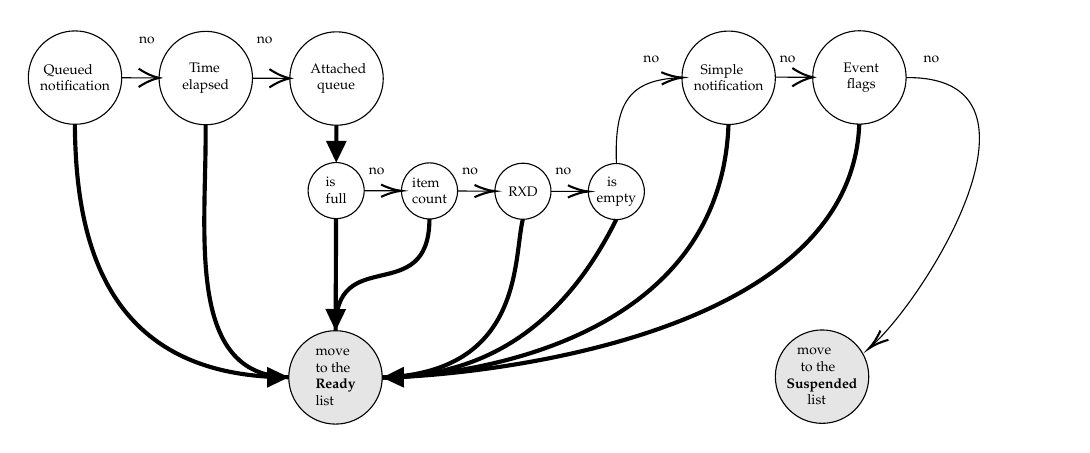
\begin{tikzpicture}[x=0.75pt,y=0.75pt,yscale=-0.9,xscale=0.9]
        \draw   (85.09,90) .. controls (71.28,89.95) and (60.05,101.11) .. (60,114.91) .. controls (59.95,128.72) and (71.11,139.95) .. (84.91,140) .. controls (98.72,140.05) and (109.95,128.89) .. (110,115.09) .. controls (110.05,101.28) and (98.89,90.05) .. (85.09,90) -- cycle ;
        \draw   (155.09,90.24) .. controls (141.28,90.2) and (130.05,101.35) .. (130,115.16) .. controls (129.95,128.96) and (141.11,140.2) .. (154.91,140.24) .. controls (168.72,140.29) and (179.95,129.14) .. (180,115.33) .. controls (180.05,101.52) and (168.89,90.29) .. (155.09,90.24) -- cycle ;
        \draw    (110,115.09) -- (128,115.15) ;
        \draw [shift={(130,115.16)}, rotate = 180.2] [color={rgb, 255:red, 0; green, 0; blue, 0 }  ][line width=0.75]    (10.93,-4.9) .. controls (6.95,-2.3) and (3.31,-0.67) .. (0,0) .. controls (3.31,0.67) and (6.95,2.3) .. (10.93,4.9)   ;
        \draw   (224.84,160.49) .. controls (216.56,160.46) and (209.82,167.15) .. (209.79,175.44) .. controls (209.76,183.72) and (216.45,190.46) .. (224.74,190.49) .. controls (233.02,190.52) and (239.76,183.82) .. (239.79,175.54) .. controls (239.82,167.26) and (233.13,160.52) .. (224.84,160.49) -- cycle ;
        \draw [line width=1.5]    (84.91,140) .. controls (85.37,197.92) and (98.51,274.01) .. (196.45,275.38) ;
        \draw [shift={(199.44,275.4)}, rotate = 539.9200000000001] [fill={rgb, 255:red, 0; green, 0; blue, 0 }  ][line width=0.08]  [draw opacity=0] (11.61,-5.58) -- (0,0) -- (11.61,5.58) -- cycle    ;
        \draw   (225.09,90.49) .. controls (211.28,90.44) and (200.05,101.59) .. (200,115.4) .. controls (199.95,129.21) and (211.1,140.44) .. (224.91,140.49) .. controls (238.72,140.54) and (249.95,129.38) .. (250,115.58) .. controls (250.05,101.77) and (238.89,90.54) .. (225.09,90.49) -- cycle ;
        \draw    (180,115.33) -- (198,115.39) ;
        \draw [shift={(200,115.4)}, rotate = 180.2] [color={rgb, 255:red, 0; green, 0; blue, 0 }  ][line width=0.75]    (10.93,-4.9) .. controls (6.95,-2.3) and (3.31,-0.67) .. (0,0) .. controls (3.31,0.67) and (6.95,2.3) .. (10.93,4.9)   ;
        \draw [line width=1.5]    (224.91,140.49) -- (224.86,156.49) ;
        \draw [shift={(224.84,160.49)}, rotate = 270.2] [fill={rgb, 255:red, 0; green, 0; blue, 0 }  ][line width=0.08]  [draw opacity=0] (11.61,-5.58) -- (0,0) -- (11.61,5.58) -- cycle    ;
        \draw   (274.84,160.66) .. controls (266.56,160.63) and (259.82,167.33) .. (259.79,175.61) .. controls (259.76,183.89) and (266.45,190.63) .. (274.74,190.66) .. controls (283.02,190.69) and (289.76,184) .. (289.79,175.72) .. controls (289.82,167.43) and (283.13,160.69) .. (274.84,160.66) -- cycle ;
        \draw    (239.79,175.54) -- (257.79,175.6) ;
        \draw [shift={(259.79,175.61)}, rotate = 180.2] [color={rgb, 255:red, 0; green, 0; blue, 0 }  ][line width=0.75]    (10.93,-3.29) .. controls (6.95,-1.4) and (3.31,-0.3) .. (0,0) .. controls (3.31,0.3) and (6.95,1.4) .. (10.93,3.29)   ;
        \draw   (324.84,160.84) .. controls (316.56,160.81) and (309.82,167.5) .. (309.79,175.79) .. controls (309.76,184.07) and (316.45,190.81) .. (324.74,190.84) .. controls (333.02,190.87) and (339.76,184.17) .. (339.79,175.89) .. controls (339.82,167.61) and (333.13,160.87) .. (324.84,160.84) -- cycle ;
        \draw [line width=1.5]    (224.74,190.49) -- (224.54,246.49) ;
        \draw [shift={(224.53,250.49)}, rotate = 270.2] [fill={rgb, 255:red, 0; green, 0; blue, 0 }  ][line width=0.08]  [draw opacity=0] (11.61,-5.58) -- (0,0) -- (11.61,5.58) -- cycle    ;
        \draw  [fill=gray!20  ,fill opacity=1 ] (224.53,250.49) .. controls (210.72,250.44) and (199.49,261.59) .. (199.44,275.4) .. controls (199.39,289.21) and (210.55,300.44) .. (224.35,300.49) .. controls (238.16,300.54) and (249.39,289.38) .. (249.44,275.57) .. controls (249.49,261.77) and (238.33,250.54) .. (224.53,250.49) -- cycle ;
        \draw   (435,90.09) .. controls (421.19,90.04) and (409.96,101.19) .. (409.91,115) .. controls (409.86,128.81) and (421.02,140.04) .. (434.83,140.09) .. controls (448.63,140.14) and (459.86,128.98) .. (459.91,115.17) .. controls (459.96,101.37) and (448.81,90.14) .. (435,90.09) -- cycle ;
        \draw    (289.79,175.72) -- (297.46,175.74) -- (307.79,175.78) ;
        \draw [shift={(309.79,175.79)}, rotate = 180.2] [color={rgb, 255:red, 0; green, 0; blue, 0 }  ][line width=0.75]    (10.93,-3.29) .. controls (6.95,-1.4) and (3.31,-0.3) .. (0,0) .. controls (3.31,0.3) and (6.95,1.4) .. (10.93,3.29)   ;
        \draw [line width=1.5]    (154.91,140.24) .. controls (155.5,197) and (143.5,275) .. (199.44,275.4) ;
        \draw [line width=1.5]    (274.74,190.66) .. controls (274.5,239) and (223.5,203) .. (224.53,250.49) ;
        \draw [line width=1.5]    (324.74,190.84) .. controls (319.5,212) and (325.5,273) .. (249.44,275.57) ;
        \draw   (374.84,161.01) .. controls (366.56,160.98) and (359.82,167.68) .. (359.79,175.96) .. controls (359.76,184.24) and (366.45,190.98) .. (374.74,191.01) .. controls (383.02,191.04) and (389.76,184.35) .. (389.79,176.06) .. controls (389.82,167.78) and (383.13,161.04) .. (374.84,161.01) -- cycle ;
        \draw    (339.79,175.89) -- (357.79,175.95) ;
        \draw [shift={(359.79,175.96)}, rotate = 180.2] [color={rgb, 255:red, 0; green, 0; blue, 0 }  ][line width=0.75]    (10.93,-3.29) .. controls (6.95,-1.4) and (3.31,-0.3) .. (0,0) .. controls (3.31,0.3) and (6.95,1.4) .. (10.93,3.29)   ;
        \draw [line width=1.5]    (374.74,191.01) .. controls (342.17,256.37) and (296.35,273.96) .. (253.42,275.48) ;
        \draw [shift={(249.44,275.57)}, rotate = 359.25] [fill={rgb, 255:red, 0; green, 0; blue, 0 }  ][line width=0.08]  [draw opacity=0] (11.61,-5.58) -- (0,0) -- (11.61,5.58) -- cycle    ;
        \draw    (374.84,161.01) .. controls (373.53,127.68) and (382.14,116.45) .. (408.29,115.07) ;
        \draw [shift={(409.91,115)}, rotate = 537.9100000000001] [color={rgb, 255:red, 0; green, 0; blue, 0 }  ][line width=0.75]    (10.93,-3.29) .. controls (6.95,-1.4) and (3.31,-0.3) .. (0,0) .. controls (3.31,0.3) and (6.95,1.4) .. (10.93,3.29)   ;
        \draw   (505,89.91) .. controls (491.19,89.86) and (479.96,101.02) .. (479.91,114.83) .. controls (479.86,128.63) and (491.02,139.86) .. (504.83,139.91) .. controls (518.63,139.96) and (529.86,128.81) .. (529.91,115) .. controls (529.96,101.19) and (518.81,89.96) .. (505,89.91) -- cycle ;
        \draw    (459.91,114.76) -- (477.91,114.82) ;
        \draw [shift={(479.91,114.83)}, rotate = 180.2] [color={rgb, 255:red, 0; green, 0; blue, 0 }  ][line width=0.75]    (10.93,-4.9) .. controls (6.95,-2.3) and (3.31,-0.67) .. (0,0) .. controls (3.31,0.67) and (6.95,2.3) .. (10.93,4.9)   ;
        \draw [line width=1.5]    (434.83,140.09) .. controls (430.5,257) and (293.5,275) .. (249.44,275.57) ;
        \draw [line width=1.5]    (504.83,139.91) .. controls (500.5,256.83) and (293.5,275) .. (249.44,275.57) ;
        \draw  [fill=gray!20 ] (485,250.09) .. controls (471.19,250.04) and (459.96,261.19) .. (459.91,275) .. controls (459.86,288.81) and (471.02,300.04) .. (484.83,300.09) .. controls (498.63,300.14) and (509.86,288.98) .. (509.91,275.17) .. controls (509.96,261.37) and (498.81,250.14) .. (485,250.09) -- cycle ;
        \draw    (529.91,115) .. controls (613.23,114.01) and (542.77,230.26) .. (511.41,258.76) ;
        \draw [shift={(510,260)}, rotate = 319.45] [color={rgb, 255:red, 0; green, 0; blue, 0 }  ][line width=0.75]    (10.93,-3.29) .. controls (6.95,-1.4) and (3.31,-0.3) .. (0,0) .. controls (3.31,0.3) and (6.95,1.4) .. (10.93,3.29)   ;
        \draw (85,115) node  [font=\tiny] [align=left] { \ Queued\\notification};
        \draw (224.79,175.49) node  [font=\tiny] [align=left] {is\\full};
        \draw (274.79,175.66) node  [font=\tiny] [align=left] {item\\count};
        \draw (324.79,175.84) node  [font=\tiny] [align=left] {RXD};
        \draw (224.44,275.49) node  [font=\tiny] [align=left] {move \\to the\\\textbf{Ready} \\list};
        \draw (374.79,176.01) node  [font=\tiny] [align=left] { \ \ \ is\\empty};
        \draw (155,115.24) node  [font=\tiny] [align=left] { \ \ Time\\elapsed};
        \draw (225,115.49) node  [font=\tiny] [align=left] { \ Attached\\ \ \ \ queue};
        \draw (434.91,115.09) node  [font=\tiny] [align=left] { \ \ Simple\\notification};
        \draw (504.91,114.91) node  [font=\tiny] [align=left] { \ Event\\ \ \ flags};
        \draw (484.91,275.09) node  [font=\tiny] [align=left] { \ \ \ move \\ \ \ \ \ to the\\\textbf{Suspended} \\ \ \ \ \ \ \ list};
        \draw (123.5,95) node  [font=\tiny] [align=left] {no};
        \draw (186.5,95) node  [font=\tiny] [align=left] {no};
        \draw (246.5,165) node  [font=\tiny] [align=left] {no};
        \draw (296.5,165) node  [font=\tiny] [align=left] {no};
        \draw (346.5,165) node  [font=\tiny] [align=left] {no};
        \draw (393.5,105) node  [font=\tiny] [align=left] {no};
        \draw (466.5,105) node  [font=\tiny] [align=left] {no};
        \draw (543.5,105) node  [font=\tiny] [align=left] {no};
    \end{tikzpicture}
    \caption{Event precedence}
    \label{fig:eventprecedence}
\end{figure}

\paragraph{Additional operational states :}
Each task has independent operating states from those globally controlled by the scheduler. These states can be handled by the application writer to modify the event-flow to the task and consequently, affecting the transition to the \textit{qReady} global state. These states are described below.

\begin{itemize}
    \item \textit{qAwake} : In this state, the task is conceptually in an alert mode, handling most of the available events. This operational state is available when the \lstinline{SHUTDOWN} bit is set, allowing the next operational states to be available:
    \begin{itemize}
        \item \textit{qEnabled} : The task is able to catch all the events. This operational state is available when the \lstinline{ENABLE} bit is set.
        \item \textit{qDisabled} : In this state the time events will be discarded. This operational state is available when the \lstinline{ENABLE} bit is cleared.
    \end{itemize}
    \item \textit{qAsleep} : Task operability is put into a deep doze mode, so the task can't be triggered by the lower precedence events.  This operational state is available when the \lstinline{SHUTDOWN} bit is cleared. The task can exit from this operational state when it receives a high precedence event (a queued notification) or using the \lstinline{qTask_Set_State()} API.
\end{itemize}

The figure \ref{fig:eventflow} shows a better representation of how the event flow can be affected by this operational states.

\begin{tcolorbox}
\HandRight Queued notifications are the only event that can wake up sleeping tasks.
\end{tcolorbox}
\begin{tcolorbox}
\HandRight The \textit{qAsleep} operational state overrides the \textit{qEnabled} and \textit{qDisabled} State.
\end{tcolorbox}

\begin{figure}[H]
    \centering
    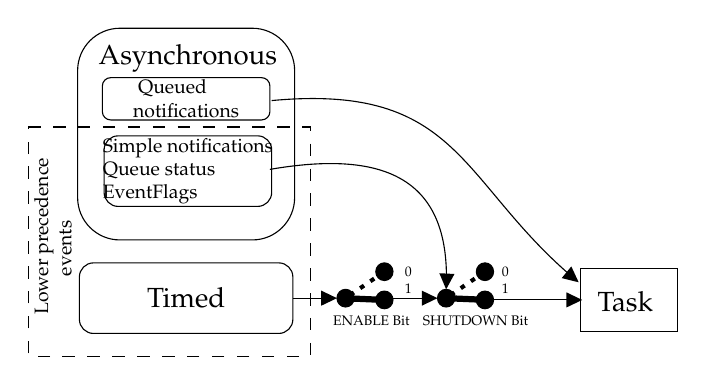
\begin{tikzpicture}[x=0.75pt,y=0.75pt,yscale=-0.85,xscale=0.85]
        \draw   (41.5,194) .. controls (41.5,189.58) and (45.08,186) .. (49.5,186) -- (154.5,186) .. controls (158.92,186) and (162.5,189.58) .. (162.5,194) -- (162.5,218) .. controls (162.5,222.42) and (158.92,226) .. (154.5,226) -- (49.5,226) .. controls (45.08,226) and (41.5,222.42) .. (41.5,218) -- cycle ;
        \draw   (40.5,77) .. controls (40.5,63.75) and (51.25,53) .. (64.5,53) -- (139.5,53) .. controls (152.75,53) and (163.5,63.75) .. (163.5,77) -- (163.5,149) .. controls (163.5,162.25) and (152.75,173) .. (139.5,173) -- (64.5,173) .. controls (51.25,173) and (40.5,162.25) .. (40.5,149) -- cycle ;
        \draw   (55.5,122) .. controls (55.5,117.58) and (59.08,114) .. (63.5,114) -- (142.5,114) .. controls (146.92,114) and (150.5,117.58) .. (150.5,122) -- (150.5,146) .. controls (150.5,150.42) and (146.92,154) .. (142.5,154) -- (63.5,154) .. controls (59.08,154) and (55.5,150.42) .. (55.5,146) -- cycle ;
        \draw   (325.5,189) -- (380.5,189) -- (380.5,225) -- (325.5,225) -- cycle ;
        \draw [line width=2.25]    (214.38,207) -- (191,206) ;
        \draw  [fill={rgb, 255:red, 0; green, 0; blue, 0 }  ,fill opacity=1 ] (187.5,206) .. controls (187.5,203.24) and (189.68,201) .. (192.38,201) .. controls (195.07,201) and (197.25,203.24) .. (197.25,206) .. controls (197.25,208.76) and (195.07,211) .. (192.38,211) .. controls (189.68,211) and (187.5,208.76) .. (187.5,206) -- cycle ;
        \draw    (324.5,207) -- (276.25,207) ;
        \draw [shift={(326.5,207)}, rotate = 180] [fill={rgb, 255:red, 0; green, 0; blue, 0 }  ][line width=0.75]  [draw opacity=0] (8.93,-4.29) -- (0,0) -- (8.93,4.29) -- cycle    ;
        \draw  [fill={rgb, 255:red, 0; green, 0; blue, 0 }  ,fill opacity=1 ] (209.5,191) .. controls (209.5,188.24) and (211.68,186) .. (214.38,186) .. controls (217.07,186) and (219.25,188.24) .. (219.25,191) .. controls (219.25,193.76) and (217.07,196) .. (214.38,196) .. controls (211.68,196) and (209.5,193.76) .. (209.5,191) -- cycle ;
        \draw  [fill={rgb, 255:red, 0; green, 0; blue, 0 }  ,fill opacity=1 ] (209.5,207) .. controls (209.5,204.24) and (211.68,202) .. (214.38,202) .. controls (217.07,202) and (219.25,204.24) .. (219.25,207) .. controls (219.25,209.76) and (217.07,212) .. (214.38,212) .. controls (211.68,212) and (209.5,209.76) .. (209.5,207) -- cycle ;
        \draw    (185.5,206) -- (162.5,206) ;
        \draw [shift={(187.5,206)}, rotate = 180] [fill={rgb, 255:red, 0; green, 0; blue, 0 }  ][line width=0.75]  [draw opacity=0] (8.93,-4.29) -- (0,0) -- (8.93,4.29) -- cycle    ;
        \draw  [fill={rgb, 255:red, 0; green, 0; blue, 0 }  ,fill opacity=1 ] (244.5,206) .. controls (244.5,203.24) and (246.68,201) .. (249.38,201) .. controls (252.07,201) and (254.25,203.24) .. (254.25,206) .. controls (254.25,208.76) and (252.07,211) .. (249.38,211) .. controls (246.68,211) and (244.5,208.76) .. (244.5,206) -- cycle ;
        \draw  [fill={rgb, 255:red, 0; green, 0; blue, 0 }  ,fill opacity=1 ] (266.5,191) .. controls (266.5,188.24) and (268.68,186) .. (271.38,186) .. controls (274.07,186) and (276.25,188.24) .. (276.25,191) .. controls (276.25,193.76) and (274.07,196) .. (271.38,196) .. controls (268.68,196) and (266.5,193.76) .. (266.5,191) -- cycle ;
        \draw  [color={rgb, 255:red, 0; green, 0; blue, 0 }  ,draw opacity=1 ][fill={rgb, 255:red, 0; green, 0; blue, 0 }  ,fill opacity=1 ] (266.5,207) .. controls (266.5,204.24) and (268.68,202) .. (271.38,202) .. controls (274.07,202) and (276.25,204.24) .. (276.25,207) .. controls (276.25,209.76) and (274.07,212) .. (271.38,212) .. controls (268.68,212) and (266.5,209.76) .. (266.5,207) -- cycle ;
        \draw    (242.5,206) -- (219.5,206) ;
        \draw [shift={(244.5,206)}, rotate = 180] [fill={rgb, 255:red, 0; green, 0; blue, 0 }  ][line width=0.75]  [draw opacity=0] (8.93,-4.29) -- (0,0) -- (8.93,4.29) -- cycle    ;
        \draw    (149.5,133) .. controls (212.86,122.11) and (251.72,136.7) .. (249.46,199.09) ;
        \draw [shift={(249.38,201)}, rotate = 272.8] [fill={rgb, 255:red, 0; green, 0; blue, 0 }  ][line width=0.75]  [draw opacity=0] (8.93,-4.29) -- (0,0) -- (8.93,4.29) -- cycle    ;
        \draw   (54.5,85.8) .. controls (54.5,83.15) and (56.65,81) .. (59.3,81) -- (144.7,81) .. controls (147.35,81) and (149.5,83.15) .. (149.5,85.8) -- (149.5,100.2) .. controls (149.5,102.85) and (147.35,105) .. (144.7,105) -- (59.3,105) .. controls (56.65,105) and (54.5,102.85) .. (54.5,100.2) -- cycle ;
        \draw    (150.5,94) .. controls (257.96,84.05) and (256.52,140.43) .. (323.49,196.16) ;
        \draw [shift={(324.5,197)}, rotate = 219.47] [fill={rgb, 255:red, 0; green, 0; blue, 0 }  ][line width=0.75]  [draw opacity=0] (8.93,-4.29) -- (0,0) -- (8.93,4.29) -- cycle    ;
        \draw  [dash pattern={on 4.5pt off 4.5pt}] (12.5,109) -- (172.5,109) -- (172.5,239) -- (12.5,239) -- cycle ;
        \draw [line width=2.25]    (272.75,207) -- (249.38,206) ;
        \draw [line width=1.5]  [dash pattern={on 1.69pt off 2.76pt}]  (214.38,191) -- (192.38,206) ;
        \draw [line width=1.5]  [dash pattern={on 1.69pt off 2.76pt}]  (271.38,191) -- (249.38,206) ;
        \draw (102,206) node  [align=left] {Timed};
        \draw (103,70) node  [align=left] {Asynchronous};
        \draw (351,208) node  [align=left] {Task};
        \draw (103,134) node [scale=0.7] [align=left] {Simple notifications\\Queue status\\EventFlags};
        \draw (102,93) node [scale=0.7] [align=left] { \ Queued \\notifications};
        \draw (207,219) node [scale=0.5] [align=left] {ENABLE Bit};
        \draw (266,219) node [scale=0.5] [align=left] {SHUTDOWN Bit};
        \draw (26.5,171) node [scale=0.7,rotate=-270] [align=left] {Lower precedence\\ \ \ \ \ \ \ \ \ events};
        \draw (228,196) node [scale=0.5] [align=left] {0\\1};
        \draw (283,196) node [scale=0.5] [align=left] {0\\1};
    \end{tikzpicture}
    \caption{Event flow according operational states}
    \label{fig:eventflow}
\end{figure}


\subsection{Getting started}
Unpack the source files and copy them into your project. Also, add a copy of the file \lstinline{qconfig.h} and modify it according to your needs. Setup your compiler include path with the corresponding OS directory. Include the header file \lstinline{QuarkTS.h} and setup the instance of the kernel using the \lstinline{qOS_Setup()} inside the main thread. Additional configuration to the target compiler may be required to add the path to the directory of header files. The code below shows a common initialization in the main source file. \\

File: \lstinline{main.c}
\begin{lstlisting}[style=CStyle]
#include "QuarkTS.h"
#define TIMER_TICK   0.001   /* 1ms */ 

void main( void ){
    /*start of hardware specific code*/
    HardwareSetup();  
    Configure_Periodic_Timer_Interrupt_1ms(); 
    /*end of hardware specific code*/
    qOS_Setup( NULL, TIMER_TICK, IdleTask_Callback ); 
    /*
    TODO: add Tasks to the scheduler scheme and run the OS
    */
}
\end{lstlisting}

In the above code, the following considerations should be taken
\begin{itemize}
    \item The function \lstinline{qOS_Setup()} must be called before any interaction with the OS.
    \item The procedure \lstinline{HardwareSetup()} should be a function with all the hardware instructions needed to initialize the target system.
    \item  The procedure \lstinline{Configure_Periodic_Timer_Interrupt_1ms()} should be a function with all the hardware instructions needed to initialize and run a timer with an overflow tick of one millisecond.
\end{itemize}

Tasks can be later added to the scheduling scheme by simply calling \lstinline{qOS_Add_Task()} or any of the other available APIs for specific purpose tasks.

\subsection{Recommended programming pattern}
A multitasking design pattern demands a better project organization. To have this attribute in your solution, code the tasks in a separate source file. A simple implementation example is presented below. \\

To make the handling of the tasks available in other contexts, nodes should be globals(see the \lstinline{extern} qualifier in \lstinline{MyAppTasks.h} header file).  Avoid implementing functionalities in a component that are not related to each other. Put any other components and globals resources in a separated source file, for example (\lstinline{ScreenDriver.h}/\lstinline{ScreenDriver.c}),  (\lstinline{Globals.h}/\lstinline{Globals.c}). These simple design tips will allow you to have a better principle of abstraction and will maximize the cohesion of the solution, improving the code readability and maintenance. \\

File: \lstinline{MyAppTasks.h}
\begin{lstlisting}[style=CStyle]
#ifndef MYAPPTASK_H
    #define MYAPPTASK_H
    
    #include "Globals.h"
    #include "QuarkTS.h"
    
    extern qTask_t CommunicationTask, HardwareCheckTask, 
                  CheckUserEventsTask, SignalAnalisysTask;
    
    void CommunicationTask_Callback( qEvent_t );
    void HardwareCheckTask_Callback( qEvent_t );
    void CheckUserEventsTask_Callback( qEvent_t );
    void SignalAnalisysTask_Callback( qEvent_t );
#endif
\end{lstlisting}

File: \lstinline{MyAppTasks.c}
\begin{lstlisting}[style=CStyle]
#include "MyAppTasks.h"

qTask_t CommunicationTask, HardwareCheckTask, 
        CheckUserEventsTask, SignalAnalisysTask;

void CommunicationTask_Callback( qEvent_t e ){
    /*
    TODO: Communication Task code
    */
}

void HardwareCheckTask_Callback( qEvent_t e ){
    /*
    TODO: Hardware Check Task code
    */
}

void CheckUserEventsTask_Callback( qEvent_t e ){
    /*
    TODO: Check User Events Task code
    */
}

void SignalAnalisysTask_Callback( qEvent_t e ){
    /*
    TODO: Signal Analisys Task code
    */
}

/*this task doesnt need an Identifier*/
void IdleTask_Callback( qEvent_t e ){ 
    /*
    TODO: Idle Task code
    */
}
\end{lstlisting}

File: \lstinline{main.c}
\begin{lstlisting}[style=CStyle]
#include "QuarkTS.h"
#include "Globals.h"
#include "MyAppTasks.h"

void interrupt OnTimerInterrupt( void ){ //hardware specific code
    qClock_SysTick();
}

void main( void ){
    /*start of hardware specific code*/
    HardwareSetup();
    Configure_Periodic_Timer_Interrupt_10ms(); 
    /*end of hardware specific code*/
    qOS_Setup( NULL, 0.01, IdleTask_Callback ); 
    qOS_Add_Task( HardwareCheckTask, HardwareCheckTask_Callback,
                  qLowest_Priority, 0.25, qPeriodic, qEnabled, NULL );
    qOS_Add_Task( SignalAnalisysTask, SignalAnalisysTask_Callback, 
                  qHigh_Priority, 0.1, 200, qEnabled, NULL );
    qOS_Add_EventTask( CheckEventsTask, CheckEventsTask_Callback, 
                       qMedium_Priority, NULL ); 
    qOS_Add_Task( CommunicationTask, CommunicationTask_Callback, 
                  qHigh_Priority, qTimeImmediate, qPeriodic, 
                  qEnabled, NULL );
    qOS_Run();
    for(;;){}
}
\end{lstlisting}


\subsection{Critical sections}
Since the kernel is non-preemptive, the only critical section that must be handled are the shared resources accessed from the ISR context. Perhaps, the most obvious way of achieving mutual exclusion is to allow the kernel to disable interrupts before it enters its critical section and then, enable interrupts after it leaves its critical section. \\

By disabling interrupts, the CPU will be unable to change the current context. This guarantees that the currently running job can use a shared resource without another context accessing it. But, disabling interrupts, is a major undertaking. At best, the system will not be able to service interrupts for the time the current job is doing in its critical section, however, in QuarkTS, these critical sections are handled as quickly as possible.  

Considering that the kernel is hardware-independent, the application writer should provide the necessary piece of code to enable and disable interrupts.

For this, the \lstinline{qCritical_SetInterruptsED()} \index{\lstinline{qCritical_SetInterruptsED}} API should be used. In this way, communication between ISR and tasks using queued notifications or data queues is performed safely. \\

\begin{lstlisting}[style=CStyle]
void qCritical_SetInterruptsED( void (*Restorer)(qUINT32_t), 
                                qUINT32_t (*Disabler)(void) );
\end{lstlisting}

\subsubsection*{Parameters:}
\begin{itemize}
    \item \lstinline{Restorer} : The function with hardware specific code to enable or restore interrupts.
    \item \lstinline{Disabler} : The function with hardware specific code that disables interrupts.
\end{itemize}

In some systems, disabling the global IRQ flags is not enough, as they don't save/restore state of interrupt, so here, the \lstinline{qUINT32_t} argument and return value in both functions (\lstinline{Disabler} and \lstinline{Restorer}) becomes relevant, because they can be used by the application writer to save and restore the current interrupt configuration. So, when a critical section is performed, the \lstinline{Disabler}, in addition to disable the interrupts, return the current configuration to be retained by the kernel, later when the critical section finish, this retained value is passed to \lstinline{Restorer} to bring back the saved configuration. 

\subsection{Task management APIs in run-time }
Most of the scheduling parameters regarding task execution can be changed at run-time. The following APIs are intended for this purpose. \\


\begin{lstlisting}[style=CStyle]
void qTask_Set_Time( qTask_t * const Task, const qTime_t Value )
\end{lstlisting}

Set/Change the task execution interval. \index{\lstinline{qTask_Set_Time}}

\subsubsection*{Parameters:}
\begin{itemize}
    \item \lstinline{Task} : A pointer to the task node.
    \item \lstinline{Value} : Execution interval defined in seconds (floating-point format). For immediate execution use \lstinline{qTimeImmediate}.
\end{itemize}

\noindent\hrulefill

\begin{lstlisting}[style=CStyle]
void qTask_Set_Iterations( qTask_t * const Task, qIteration_t Value )
\end{lstlisting}

Set/Change the number of task iterations. \index{\lstinline{qTask_Set_Iterations}}

\subsubsection*{Parameters:}
\begin{itemize}
    \item \lstinline{Task} : A pointer to the task node.
    \item \lstinline{Value} : Number of task executions (integer value). For indefinite execution user \lstinline{qPeriodic} or \lstinline{qIndefinite}. Tasks do not remember the number of iteration set initially. 
\end{itemize}

\noindent\hrulefill


\begin{lstlisting}[style=CStyle]
void qTask_Set_Priority( qTask_t * const Task, qPriority_t Value )
\end{lstlisting}

Set/Change the task priority value. \index{\lstinline{qTask_Set_Priority}}

\subsubsection*{Parameters:}
\begin{itemize}
    \item \lstinline{Task} : A pointer to the task node.
    \item \lstinline{Value} : Priority value. \lstinline{[0(min) - Q_PRIORITY_LEVELS(max)]}. 
\end{itemize}

\noindent\hrulefill


\begin{lstlisting}[style=CStyle]
void qTask_Set_Callback( qTask_t * const Task, qTaskFcn_t CallbackFcn )
\end{lstlisting}

Set/Change the task callback function. \index{\lstinline{qTask_Set_Callback}}. Can be used to detach an state machine.

\subsubsection*{Parameters:}
\begin{itemize}
    \item \lstinline{Task} : A pointer to the task node.
    \item \lstinline{Callback} : A pointer to a void callback method with a \lstinline{qEvent_t} parameter as input argument.
\end{itemize}

\noindent\hrulefill


\begin{lstlisting}[style=CStyle]
void qTask_Set_State( qTask_t * const Task, const qState_t State ) 
void qTask_Resume( qTask_t * const Task ) 
void qTask_Suspend( qTask_t * const Task )
void qTask_ASleep( qTask_t * const Task )
void qTask_Awake( qTask_t * const Task )
\end{lstlisting}\index{\lstinline{qTask_Resume}} \index{\lstinline{qTask_Suspend}} \index{\lstinline{qTask_ASleep}} \index{\lstinline{qTask_Awake}}

Set the task operability state. \index{\lstinline{qTask_Set_State}} \index{\lstinline{qTask_Resume}} \index{\lstinline{qTask_Suspend}}

\subsubsection*{Parameters:}
\begin{itemize}
    \item \lstinline{Task} : A pointer to the task node.
    \item \lstinline{State} : Use one of the following values:
    \begin{itemize}
        \item \lstinline{qEnabled} : Task will be able to catch all the events.
        \item \lstinline{qDisabled} : Time events will be ignored. Only asynchronous events are allowed.
        \item \lstinline{qAsleep} : The task can't be triggered by lower precedence events. Only the queued notifications events can be caught.
        \item \lstinline{qAwake} : Task will be able to catch all the events.
    \end{itemize}
\end{itemize}

\noindent\hrulefill


\begin{lstlisting}[style=CStyle]
void qTask_Set_Data( qTask_t * const Task, void* UserData )
\end{lstlisting}

Set the task data. \index{\lstinline{qTask_Set_Data}}

\subsubsection*{Parameters:}
\begin{itemize}
    \item \lstinline{Task} : A pointer to the task node.
    \item \lstinline{UserData} : A pointer to the associated data.
\end{itemize}

\noindent\hrulefill


\begin{lstlisting}[style=CStyle]
void qTask_ClearTimeElapsed( qTask_t * const Task )
\end{lstlisting}

Clear the elapsed time of the task. Restart the internal task tick. \index{\lstinline{qTask_ClearTimeElapsed}}

\subsubsection*{Parameters:}
\begin{itemize}
    \item \lstinline{Task} : A pointer to the task node.
\end{itemize}

\noindent\hrulefill


\begin{lstlisting}[style=CStyle]
qCycles_t qTask_Get_Cycles( const qTask_t * const Task )
\end{lstlisting}

Retrieve the number of task activation's. \index{\lstinline{qTask_Get_Cycles}}

\subsubsection*{Parameters:}
\begin{itemize}
    \item \lstinline{Task} : A pointer to the task node.
\end{itemize}


\subsubsection*{Return value:}
A \lstinline{qUINT32_t} value containing the number of task activations.

\noindent\hrulefill


\begin{lstlisting}[style=CStyle]
qState_t qTask_Get_State( const qTask_t * const Task )
\end{lstlisting}

Retrieve the task operational state. \index{\lstinline{qTask_Get_State}}

\subsubsection*{Parameters:}
\begin{itemize}
    \item \lstinline{Task} : A pointer to the task node.
\end{itemize}


\subsubsection*{Return value:}
\lstinline{qEnabled} or \lstinline{qDisabled} if the task is \lstinline{qAwaken}. \lstinline{qAsleep} if the task is in a sleep operational state.

\noindent\hrulefill


\begin{lstlisting}[style=CStyle]
qTask_t* qTask_Self( void )
\end{lstlisting}

Get current running task handle. \index{\lstinline{qTask_Self}}

\subsubsection*{Return value:}
A pointer to the current running task. \lstinline{NULL} when the scheduler it's in a busy state or when idle-task is running.


\noindent\hrulefill


\begin{lstlisting}[style=CStyle]
qTask_GlobalState_t qTask_Get_GlobalState( const qTask_t * const Task )
\end{lstlisting}

Retrieve the task global-state. \index{\lstinline{qTask_Get_GlobalState}}

\subsubsection*{Parameters:}
\begin{itemize}
    \item \lstinline{Task} : A pointer to the task node.
\end{itemize}


\subsubsection*{Return value:}
One of the available global states : \lstinline{qWaiting}, \lstinline{qSuspended}, \lstinline{qRunning} or \lstinline{qReady}.
Return \lstinline{qUndefinedGlobalState} if the current task its passing through a current kernel transaction

\noindent\hrulefill

\begin{lstlisting}[style=CStyle]
qBool_t qTask_HasPendingNotifications( const qTask_t * const Task  )
\end{lstlisting}

Check if the task has pending notifications. Please read section \ref{osnotifications}. \index{\lstinline{qTask_HasPendingNotifications}}

\subsubsection*{Parameters:}
\begin{itemize}
    \item \lstinline{Task} : A pointer to the task node.
\end{itemize}

\subsubsection*{Return value:}
\lstinline{qTrue} if the functon asserts, otherwise returns \lstinline{qFalse}.

\subsection{Demonstrative examples}
\subsubsection{A simple scheduling}
This example demonstrates a simple environment setup for multiple tasks. Initially, only \lstinline{task1} and \lstinline{task2} are enabled. \lstinline{task1} runs every 2 seconds 10 times and then stops. \lstinline{task2} runs every 3 seconds indefinitely. \lstinline{task1} enables \lstinline{task3} at its first run. \lstinline{task3} run every 5 seconds. \lstinline{task1} disables \lstinline{task3} on its last iteration and changed \lstinline{task2} to run every 1/2 seconds. In the end, \lstinline{task2} is the only task running every 1/2 seconds. \\

\begin{lstlisting}[style=CStyle]
#include <stdio.h>
#include <stdlib.h>
#include <stdint.h>
#include "BSP.h"

#include "QuarkTS.h"
#define TIMER_TICK   0.001   /* 1ms */ 

qTask_t task1, task2, task3; /*task nodes*/
/*==================================================================*/
void interrupt Timer0_ISR( void ) {
    qClock_SysTick();   
}
/*==================================================================*/
void Task1_Callback( qEvent_t e ){
    BSP_UART1_WriteString( "Task1" );

    if( e->FirstIteration ){
        qTask_Resume( &Task3 );    
    }
    
    if( e->LastIteration ){
        qTask_Suspend( &Task3 );
        qTask_Set_Time( &Task2, 0.5 );
    }
}
/*==================================================================*/
void Task2_Callback( qEvent_t e ){
    BSP_UART1_WriteString( "Task2" );
}
/*==================================================================*/
void Task3_Callback( qEvent_t e ){
    BSP_UART1_WriteString( "Task3" );
}
/*==================================================================*/
int main( void ) {    
    HardwareSetup();  /*hardware initialization function*/
    /*function to fire an interrupt at 1ms - timer tick*/
    Configure_Periodic_Timer0_Interrupt_1ms(); 
    
    qOS_Setup( NULL, TIMER_TICK, NULL );     
    qOS_Add_Task( &Task1, Task1_Callback, 50, 2.0, 10, qEnabled, NULL );
    qOS_Add_Task( &Task2, Task2_Callback, 50, 3.0, qPeriodic, qEnabled, NULL );
    qOS_Add_Task( &Task2, Task3_Callback, 50, 5.0, qPeriodic, qDisabled, NULL );
    qOS_Run();
	
    return 0;
}
\end{lstlisting}

\subsubsection{Using the task argument}
As seen in section \ref{addtask}, tasks can accept a parameter of type pointer to void (\lstinline{void*}). 
This parameter could be used for multiple applications, including storage, task identification, duplication removal and others. The following example shows the usage of this argument to avoid callback duplication among tasks with the same behavior. 

Consider a scenario where you have to build a digital controller for many physical variables, for example, a PID controller for temperature, humidity and light. The PID algorithm will be the same for all variables. The only difference will be the variable input, the controlled output action and the PID gains. In this case, each of the PID tasks will utilize the same callback methods. The only difference will be the I/O parameters (specific for each PID controller). \\

Let's define a PID data structure with the I/O variables and gains. \\
 
\begin{lstlisting}[style=CStyle]
   typedef struct{
        float yt; /*Measured variable (Controller Input)*/
        float ut; /*Controlled variable (Controller Output)*/
        float ie; /*Accumulated error*/
        float pe; /*Previous error*/
        float dt; /*Controller Time Step*/
        float sp; /*Set-Point*/
        float Kc, Ki, Kd; /*PID Gains*/ 
    }PID_Params_t;
    
    PID_Params_t TemperatureControl = {
       0,0,0,0, /*Initial IO state of yt and ut*/
       1.5, /*time step*/
       28.5, /*Set-Point*/
       0.89, 0.122, 0.001 /*Kc, Ki, Kd*/
    };
    PID_Params_t HumidityControl= {
       0,0,0,0, /*Initial IO state of yt and ut*/
       1, /*time step*/
       60.0, /*Set-Point*/
       2.5, 0.2354, 0.0015 /*Kc, Ki, Kd*/
    };
    PID_Params_t LightControl= {
       0,0,0,0, /*Initial IO state of yt and ut*/
       0.5, /*time step*/
       45.0, /*Set-Point*/
       5.36, 0.0891, 0.0 /*Kc, Ki, Kd*/
    };
\end{lstlisting}

A task will be added to the scheme to collect the sensor data and apply the respective control output. \\

\begin{lstlisting}[style=CStyle]
qOS_Add_Task( &IO_TASK, IO_TASK_Callback, qMedium_Priority, 0.1, qPeriodic, 
              qEnabled, "iotask");
\end{lstlisting}

\begin{lstlisting}[style=CStyle]
void IO_TASK_Callback( qEvent_t e ){
    TemperatureControl.yt  = SampleTemperatureSensor();
    HumidityControl.yt  = SampleHumiditySensor();
    LightControl.yt  = SampleLightSensor();
    WriteTemperatureActuatorValue( TemperatureControl.ut );
    WriteHumidityActuatorValue( HumidityControl.ut );
    WriteLightActuatorValue( LightControl.ut ); 
}
\end{lstlisting}

Then, three different tasks are created to apply the respective PID controller. Note that these tasks refer to the same callback methods and we assign pointers to the respective variables. \\

\begin{lstlisting}[style=CStyle]
qOS_Add_Task( &TEMPERATURE_CONTROL_TASK, PIDControl_Callback,
              qHigh_Priority, TemperatureControl.dt , 
              qPeriodic, qEnabled, &TemperatureControl );
qOS_Add_Task( &HUMIDITY_CONTROL_TASK, PIDControl_Callback, 
              qHigh_Priority, HumidityControl.dt, 
              qPeriodic, qEnabled, &HumidityControl );
qOS_Add_Task( &LIGHT_CONTROL_TASK, PIDControl_Callback, 
              qHigh_Priority, LightControl.dt, 
              qPeriodic, qEnabled, &LightControl );
\end{lstlisting}

\begin{lstlisting}[style=CStyle]
void PIDControl_Callback( qEvent_t e ){
    float Error, derivative;
    /* 
    Obtain the reference to the specific PID controller 
    using the TaskData field from the qEvent structure
    */
    PID_Params_t *Controller = (PID_Params_t *)e->TaskData; 
    /*Compute the error*/
    Error = Controller->sp - Controller->yt;
    /*Compute the accumulated error using backward integral approximation*/
    Controller->ie += Error*Controller->dt;
    /*update and compute the derivative term*/
    derivative = (Error - Controller->pe)/Controller->dt;
    /*update the previous error*/
    Controller->pe = Error;
    /*compute the pid control law*/
    Controller->ut = Controller->Kc*Error  +  
                     Controller->Ki*Controller->ie + 
                     Controller->Kd*derivative;
}
\end{lstlisting}

\newpage

\subsection{Configuration macros}
Some  OS features can be customized using a set of macros located in the header file \lstinline{qconfig.h}. Here is the default configuration, followed by an explanation of each macro: \\

\begin{adjustbox}{width=\textwidth,totalheight={18cm}}
\begin{tabularx}
{\textwidth}{l X}
\hline
{\lstinline!Q_PRIORITY_LEVELS!} & \textit{Default:} {\lstinline!3!}.  The number of priorities available for application tasks.\\
\hline
{\lstinline!Q_SETUP_TIME_CANONICAL!} & \textit{Default:}
{\lstinline!0(disabled)!}. If enabled, the kernel assumes the timing base to 1mS(1KHz). So all time specifications for tasks and STimers must be set in milliseconds(mS). Also can be used to remove the floating-point operations when dealing with time. In some systems, can reduce the memory usage. \\
\hline
{\lstinline!Q_SETUP_TICK_IN_HERTZ!} & \textit{Default:} {\lstinline!0(disabled)!}. If enabled, the timing base will be taken as frequency(Hz) instead of period(S) by {\lstinline!qOS_Setup()!} (In some systems, can reduce the memory usage ). \\
\hline
{\lstinline!Q_PRIO_QUEUE_SIZE!} & \textit{Default:} {\lstinline!10!}.  Size of the priority queue for notifications. This argument should be an integer number greater than zero. A zero value can be used to disable this functionality.\\
\hline
{\lstinline!Q_PRESERVE_TASK_ENTRY_ORDER !} & \textit{Default:} {\lstinline!0(disabled)!}. If enabled, kernel will preserve the tasks entry order every OS scheduling cycle.\\
\hline
{\lstinline!Q_MEMORY_MANAGER!} & \textit{Default:} {\lstinline!1(enabled)!}. Used to enable or disable the memory management module. \\
\hline
{\lstinline!Q_BYTE_ALIGNMENT!} & \textit{Default:} {\lstinline!8!}. Used by the memory management module to peform the byte-aligment. \\
\hline
{\lstinline!Q_DEFAULT_HEAP_SIZE!} & \textit{Default:} {\lstinline!2048!}. The total amount of heap size for the default memory pool. \\
\hline
{\lstinline!Q_NOTIFICATION_SPREADER!} & \textit{Default:} {\lstinline!0(disabled)!}. Used to enable or disable the spread notification functionality. \\
\hline
{\lstinline!Q_FSM!} & \textit{Default:} {\lstinline!1(enabled)!}.  Used to enable or disable the Finite State Machine (FSM) extension. \\
\hline
{\lstinline!Q_QUEUES!} & \textit{Default:} {\lstinline!1(enabled)!}.  Used to enable or disable the queues APIs for communication to tasks. \\
\hline
{\lstinline!Q_TRACE_VARIABLES!} & \textit{Default:} {\lstinline!1(enabled)!}.  Used to enable or disable  debug and trace macros.\\
\hline
{\lstinline!Q_DEBUGTRACE_BUFSIZE!} & \textit{Default:} {\lstinline!36!}. The buffer size for debug and trace macros.\\
\hline
{\lstinline!Q_DEBUGTRACE_FULL!} & \textit{Default:} {\lstinline!1(enabled)!}. Used to enable of disable the extended output of trace macros.\\
\hline
{\lstinline!Q_ATCLI!} & \textit{Default:} {\lstinline!1(enabled)!}. Used to enable or disable the AT Command Line Interface (CLI) module. \\
\hline
{\lstinline!Q_TASK_COUNT_CYCLES!} & \textit{Default:} {\lstinline!0(disabled)!}. Used to enable or disable the cycle count in tasks. \\
\hline
{\lstinline!Q_TASK_EVENT_FLAGS!} & \textit{Default:} {\lstinline!1(enabled)!}. Used to enable or disable the task event flags.\\
\hline
{\lstinline!Q_MAX_FTOA_PRECISION!} & \textit{Default:} {\lstinline!10!}. The default precision used to perform float to ASCII conversions. \\
\hline
{\lstinline!Q_ATOF_FULL!} & \textit{Default:} {\lstinline!0(disabled)!}. Used to enable or disable the scientific notation in ASCII to float conversions. \\
\hline
{\lstinline!Q_ALLOW_SCHEDULER_RELEASE!} & \textit{Default:} {\lstinline!0(disabled)!}. Used to enable or disable the scheduler release functionality. \\
\hline
{\lstinline!Q_RESPONSE_HANDLER!} & \textit{Default:} {\lstinline!1(enabled)!}. Used to enable or disable the response handler functionality. \\
\hline
{\lstinline!Q_EDGE_CHECK_IOGROUPS!} & \textit{Default:} {\lstinline!1(enabled)!}. Used to enable or disable the edge check functionality for I/O groups . \\
\hline
{\lstinline!Q_BYTE_SIZED_BUFFERS!} & \textit{Default:} {\lstinline!1(enabled)!}. Used to enable or disable the usage of Byte-sized buffers. \\
\hline
\end{tabularx}
\end{adjustbox}

\newpage

\section{Events} \label{events}
\subsection{Time elapsed}
Running tasks at pre-determined rates is desirable in many situations, like sensory data acquisition, low-level servoing, control loops, action planning and system monitoring. As seen in section \ref{addtask}, you can schedule tasks at any interval your design demands, at least, if the time specification is lower than the scheduler tick. When an application consists of several periodic tasks with individual timing constraints, a few points must be taken:

\begin{itemize}
    \item When the time interval of a certain task has elapsed, the scheduler triggers an event (\textit{byTimeElapsed}) that put the task in a \lstinline{qReady} state  (see figure ~\ref{fig:timelag}).
    \item If a task has a finite number iterations, the scheduler will disable the task when the number of iterations reaches the programmed value.
    \item Tasks always have an inherent time-lag that can be noticed even more, when the programmed time-interval is too low (see figure ~\ref{fig:timelag}). In a real-time context, it is important to reduce this time-lag or jitter, to an acceptable level for the application. 
    \begin{tcolorbox}
    \HandRight QuarkTS can generally meet a time deadline if you use lightweight code in the callbacks and there is a reduced pool of pending tasks, so it can be considered a soft real-time scheduler, however,  it cannot meet a deadline deterministically like a hard real-time OS.
    \end{tcolorbox}

    \begin{figure}[H]
    \centering
    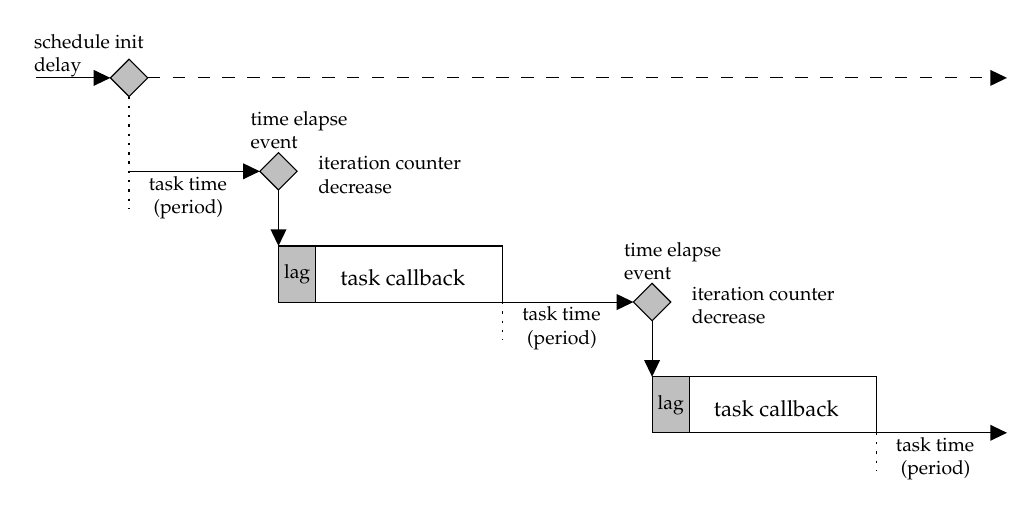
\begin{tikzpicture}[x=0.75pt,y=0.75pt,yscale=-1,xscale=1,scale=0.9]
        \draw  [fill=lightgray,fill opacity=1 ] (130,20) -- (140,30) -- (130,40) -- (120,30) -- cycle ;
        \draw    (80,30) -- (118,30) ;
        \draw [shift={(120,30)}, rotate = 180] [fill=black][line width=0.75]  [draw opacity=0] (8.93,-4.29) -- (0,0) -- (8.93,4.29) -- cycle;
        \draw  [dash pattern={on 4.5pt off 4.5pt}]  (140,30) -- (598,30) ;
        \draw [shift={(600,30)}, rotate = 180] [fill=black][line width=0.75]  [draw opacity=0] (8.93,-4.29) -- (0,0) -- (8.93,4.29) -- cycle;
        \draw  [dash pattern={on 0.84pt off 2.51pt}]  (130,40) -- (130,100) ;
        \draw    (130,80) -- (198,80) ;
        \draw [shift={(200,80)}, rotate = 180] [fill=black][line width=0.75]  [draw opacity=0] (8.93,-4.29) -- (0,0) -- (8.93,4.29) -- cycle;
        \draw  [fill=lightgray,fill opacity=1 ] (210,70) -- (220,80) -- (210,90) -- (200,80) -- cycle ;
        \draw  [fill=lightgray,fill opacity=1 ] (210,120) -- (230,120) -- (230,150) -- (210,150) -- cycle ;
        \draw   (230,120) -- (330,120) -- (330,150) -- (230,150) -- cycle ;
        \draw    (210,90) -- (210,118) ;
        \draw [shift={(210,120)}, rotate = 270] [fill=black][line width=0.75]  [draw opacity=0] (8.93,-4.29) -- (0,0) -- (8.93,4.29) -- cycle;
        \draw  [dash pattern={on 0.84pt off 2.51pt}]  (330,150) -- (330,170) ;
        \draw    (330,150) -- (398,150) ;
        \draw [shift={(400,150)}, rotate = 180] [fill=black][line width=0.75]  [draw opacity=0] (8.93,-4.29) -- (0,0) -- (8.93,4.29) -- cycle;
        \draw  [fill=lightgray,fill opacity=1 ] (410,140) -- (420,150) -- (410,160) -- (400,150) -- cycle ;
        \draw  [fill=lightgray,fill opacity=1 ] (410,190) -- (430,190) -- (430,220) -- (410,220) -- cycle ;
        \draw   (430,190) -- (530,190) -- (530,220) -- (430,220) -- cycle ;
        \draw    (410,160) -- (410,188) ;
        \draw [shift={(410,190)}, rotate = 270] [fill=black][line width=0.75]  [draw opacity=0] (8.93,-4.29) -- (0,0) -- (8.93,4.29) -- cycle;
        \draw  [dash pattern={on 0.84pt off 2.51pt}]  (530,220) -- (530,240) ;
        \draw    (530,220) -- (598,220) ;
        \draw [shift={(600,220)}, rotate = 180] [fill=black][line width=0.75]  [draw opacity=0] (8.93,-4.29) -- (0,0) -- (8.93,4.29) -- cycle;
        \draw (108.5,18) node [scale=0.7] [align=left] {schedule init\\delay};
        \draw (221,58) node [scale=0.7] [align=left] {time elapse\\event};
        \draw (220,135) node [scale=0.7] [align=left] {lag};
        \draw (276.5,137) node [scale=0.8] [align=left] {task callback};
        \draw (269.5,82) node [scale=0.7] [align=left] {iteration counter\\decrease};
        \draw (161.5,94) node [scale=0.7] [align=left] { task time\\ \ (period)};
        \draw (421,128) node [scale=0.7] [align=left] {time elapse\\event};
        \draw (420,205) node [scale=0.7] [align=left] {lag};
        \draw (476.5,207) node [scale=0.8] [align=left] {task callback};
        \draw (469.5,152) node [scale=0.7] [align=left] {iteration counter\\decrease};
        \draw (361.5,164) node [scale=0.7] [align=left] { task time\\ \ (period)};
        \draw (561.5,234) node [scale=0.7] [align=left] { task time\\ \ (period)};
    \end{tikzpicture}
    \caption{Inherit time lag}
    \label{fig:timelag}
\end{figure}

    \item The most significant delay times are produced inside the callbacks. As mentioned before, use short efficient callback methods written for cooperative scheduling.
    \item If two tasks have the same time-interval, the scheduler executes first, the task with the highest priority value (see figure \ref{fig:timelapsed}).

    \begin{figure}[H]
    \centering
        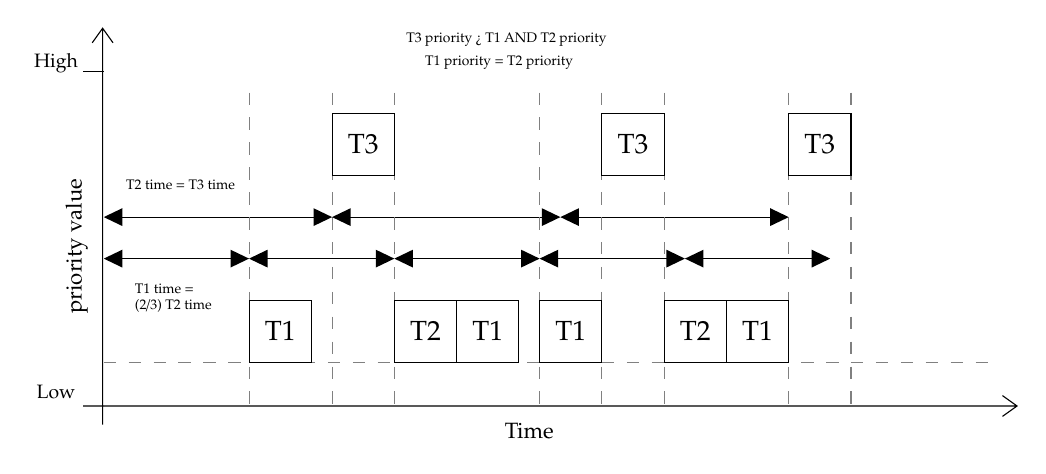
\begin{tikzpicture}[x=0.75pt,y=0.75pt,yscale=-1,xscale=1]
        \draw  (50,241) -- (500,241)(59.45,59) -- (59.45,250) (493,236) -- (500,241) -- (493,246) (54.45,66) -- (59.45,59) -- (64.45,66)  ;
        \draw    (50,80) -- (60,80) ;
        \draw [color=gray  ,draw opacity=1 ] [dash pattern={on 4.5pt off 4.5pt}]  (60,220) -- (490,220) ;
        \draw [color=gray  ,draw opacity=1 ] [dash pattern={on 4.5pt off 4.5pt}]  (170,90) -- (170,240) ;
        \draw    (62,170) -- (128,170) ;
        \draw [shift={(130,170)}, rotate = 180] [fill=black][line width=0.75]  [draw opacity=0] (8.93,-4.29) -- (0,0) -- (8.93,4.29) -- cycle;
        \draw [shift={(60,170)}, rotate = 0] [fill=black][line width=0.75]  [draw opacity=0] (8.93,-4.29) -- (0,0) -- (8.93,4.29) -- cycle ;
        \draw  [fill=white  ,fill opacity=1 ] (230,190) -- (260,190) -- (260,220) -- (230,220) -- cycle ;
        \draw    (62,150) -- (168,150) ;
        \draw [shift={(170,150)}, rotate = 180] [fill=black][line width=0.75][draw opacity=0] (8.93,-4.29) -- (0,0) -- (8.93,4.29) -- cycle;
        \draw [shift={(60,150)}, rotate = 0] [fill=black][line width=0.75]  [draw opacity=0] (8.93,-4.29) -- (0,0) -- (8.93,4.29) -- cycle;
        \draw    (172,150) -- (278,150) ;
        \draw [shift={(280,150)}, rotate = 180] [fill=black][line width=0.75][draw opacity=0] (8.93,-4.29) -- (0,0) -- (8.93,4.29) -- cycle;
        \draw [shift={(170,150)}, rotate = 0] [fill=black][line width=0.75][draw opacity=0] (8.93,-4.29) -- (0,0) -- (8.93,4.29) -- cycle;
        \draw    (282,150) -- (388,150) ;
        \draw [shift={(390,150)}, rotate = 180] [fill=black][line width=0.75]  [draw opacity=0] (8.93,-4.29) -- (0,0) -- (8.93,4.29) -- cycle;
        \draw [shift={(280,150)}, rotate = 0] [fill=black][line width=0.75]  [draw opacity=0] (8.93,-4.29) -- (0,0) -- (8.93,4.29) -- cycle;
        \draw [color=gray  ,draw opacity=1 ] [dash pattern={on 4.5pt off 4.5pt}]  (270,90) -- (270,240) ;
        \draw [color=gray  ,draw opacity=1 ] [dash pattern={on 4.5pt off 4.5pt}]  (390,90) -- (390,240) ;
        \draw [color=gray  ,draw opacity=1 ] [dash pattern={on 4.5pt off 4.5pt}]  (200,90) -- (200,240) ;
        \draw [color=gray  ,draw opacity=1 ] [dash pattern={on 4.5pt off 4.5pt}]  (130,90) -- (130,240) ;
        \draw [color=gray  ,draw opacity=1 ] [dash pattern={on 4.5pt off 4.5pt}]  (300,90) -- (300,240) ;
        \draw    (132,170) -- (198,170) ;
        \draw [shift={(200,170)}, rotate = 180] [fill=black][line width=0.75][draw opacity=0] (8.93,-4.29) -- (0,0) -- (8.93,4.29) -- cycle;
        \draw [shift={(130,170)}, rotate = 0] [fill=black][line width=0.75][draw opacity=0] (8.93,-4.29) -- (0,0) -- (8.93,4.29) -- cycle;
        \draw    (202,170) -- (268,170) ;
        \draw [shift={(270,170)}, rotate = 180] [fill=black][line width=0.75][draw opacity=0] (8.93,-4.29) -- (0,0) -- (8.93,4.29) -- cycle;
        \draw [shift={(200,170)}, rotate = 0] [fill=black][line width=0.75][draw opacity=0] (8.93,-4.29) -- (0,0) -- (8.93,4.29) -- cycle;
        \draw    (272,170) -- (338,170) ;
        \draw [shift={(340,170)}, rotate = 180] [fill=black][line width=0.75][draw opacity=0] (8.93,-4.29) -- (0,0) -- (8.93,4.29) -- cycle;
        \draw [shift={(270,170)}, rotate = 0] [fill=black][line width=0.75][draw opacity=0] (8.93,-4.29) -- (0,0) -- (8.93,4.29) -- cycle;
        \draw    (342,170) -- (408,170) ;
        \draw [shift={(410,170)}, rotate = 180] [fill=black][line width=0.75]  [draw opacity=0] (8.93,-4.29) -- (0,0) -- (8.93,4.29) -- cycle;
        \draw [shift={(340,170)}, rotate = 0] [fill=black  ][line width=0.75]  [draw opacity=0] (8.93,-4.29) -- (0,0) -- (8.93,4.29) -- cycle;
        \draw  [fill=white  ,fill opacity=1 ] (270,190) -- (300,190) -- (300,220) -- (270,220) -- cycle ;
        \draw [color=gray  ,draw opacity=1 ] [dash pattern={on 4.5pt off 4.5pt}]  (330,90) -- (330,240) ;
        \draw  [fill=white  ,fill opacity=1 ] (300,100) -- (330,100) -- (330,130) -- (300,130) -- cycle ;
        \draw  [fill=white  ,fill opacity=1 ] (170,100) -- (200,100) -- (200,130) -- (170,130) -- cycle ;
        \draw  [fill=white  ,fill opacity=1 ] (200,190) -- (230,190) -- (230,220) -- (200,220) -- cycle ;
        \draw [color=gray  ,draw opacity=1 ] [dash pattern={on 4.5pt off 4.5pt}]  (420,90) -- (420,240) ;
        \draw  [fill=white  ,fill opacity=1 ] (330,190) -- (360,190) -- (360,220) -- (330,220) -- cycle ;
        \draw  [fill=white  ,fill opacity=1 ] (390,100) -- (420,100) -- (420,130) -- (390,130) -- cycle ;
        \draw  [fill=white  ,fill opacity=1 ] (130,190) -- (160,190) -- (160,220) -- (130,220) -- cycle ;
        \draw  [fill=white  ,fill opacity=1 ] (360,190) -- (390,190) -- (390,220) -- (360,220) -- cycle ;
        \draw (47,164) node [scale=0.8,rotate=-270] [align=left] {priority value};
        \draw (265,253) node [scale=0.8] [align=left] {Time};
        \draw (37,76) node [scale=0.7] [align=left] {High};
        \draw (37,234) node [scale=0.7] [align=left] {Low};
        \draw (245,205) node  [align=left] {T1};
        \draw (185,115) node  [align=left] {T3};
        \draw (215,205) node  [align=left] {T2};
        \draw (285,205) node  [align=left] {T1};
        \draw (315,115) node  [align=left] {T3};
        \draw (405,115) node  [align=left] {T3};
        \draw (145,205) node  [align=left] {T1};
        \draw (97,134.5) node [scale=0.5] [align=left] {T2 time = T3 time};
        \draw (254,64.5) node [scale=0.5] [align=left] {T3 priority > T1 AND T2 priority};
        \draw (250.5,75.5) node [scale=0.5] [align=left] {T1 priority = T2 priority};
        \draw (93.5,189) node [scale=0.5] [align=left] {T1 time = \\(2/3) T2 time};
        \draw (345,205) node  [align=left] {T2};
        \draw (375,205) node  [align=left] {T1};
    \end{tikzpicture}
    \caption{Priority scheduling example with three (3) tasks attached triggered by time-elapsed events}
    \label{fig:timelapsed}
\end{figure}

\end{itemize}
\subsection{Asynchronous events and inter-task communication}
Applications existing in heavy environments require tasks and ISR interacting with each other, forcing the application to implement some event model.
Here, we understand events, as any identifiable occurrence that has significance for the embedded system. As such, events include changes in hardware, user-generated actions or messages coming from components of the application itself.

\begin{figure}[H]
    \centering
    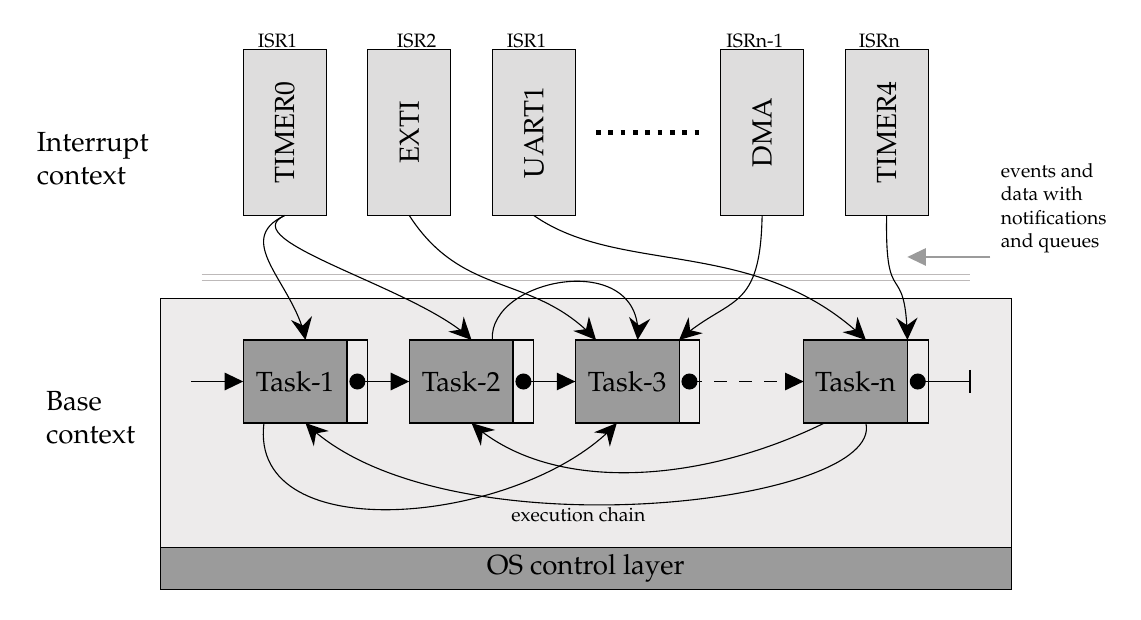
\begin{tikzpicture}[x=0.75pt,y=0.75pt,yscale=-1,xscale=1,scale=1]
        \draw  [fill={rgb, 255:red, 237; green, 235; blue, 235 }  ,fill opacity=1 ] (170,200) -- (580,200) -- (580,340) -- (170,340) -- cycle ;
        \draw  [fill={rgb, 255:red, 222; green, 221; blue, 221 }  ,fill opacity=1 ] (210,80) -- (250,80) -- (250,160) -- (210,160) -- cycle ;
        \draw  [fill={rgb, 255:red, 222; green, 221; blue, 221 }  ,fill opacity=1 ] (270,80) -- (310,80) -- (310,160) -- (270,160) -- cycle ;
        \draw  [fill={rgb, 255:red, 222; green, 221; blue, 221 }  ,fill opacity=1 ] (330,80) -- (370,80) -- (370,160) -- (330,160) -- cycle ;
        \draw  [fill={rgb, 255:red, 222; green, 221; blue, 221 }  ,fill opacity=1 ] (440,80) -- (480,80) -- (480,160) -- (440,160) -- cycle ;
        \draw  [fill={rgb, 255:red, 222; green, 221; blue, 221 }  ,fill opacity=1 ] (500,80) -- (540,80) -- (540,160) -- (500,160) -- cycle ;
        \draw [line width=1.5]  [dash pattern={on 1.69pt off 2.76pt}]  (380,120) -- (430,120) ;
        \draw  [fill={rgb, 255:red, 155; green, 155; blue, 155 }  ,fill opacity=1 ] (210,220) -- (260,220) -- (260,260) -- (210,260) -- cycle ;
        \draw   (260,220) -- (270,220) -- (270,260) -- (260,260) -- cycle ;
        \draw  [fill={rgb, 255:red, 155; green, 155; blue, 155 }  ,fill opacity=1 ] (290,220) -- (340,220) -- (340,260) -- (290,260) -- cycle ;
        \draw   (340,220) -- (350,220) -- (350,260) -- (340,260) -- cycle ;
        \draw  [fill={rgb, 255:red, 155; green, 155; blue, 155 }  ,fill opacity=1 ] (370,220) -- (420,220) -- (420,260) -- (370,260) -- cycle ;
        \draw   (420,220) -- (430,220) -- (430,260) -- (420,260) -- cycle ;
        \draw  [fill={rgb, 255:red, 155; green, 155; blue, 155 }  ,fill opacity=1 ] (480,220) -- (530,220) -- (530,260) -- (480,260) -- cycle ;
        \draw   (530,220) -- (540,220) -- (540,260) -- (530,260) -- cycle ;
        \draw    (265,240) -- (288,240) ;
        \draw [shift={(290,240)}, rotate = 180] [fill={rgb, 255:red, 0; green, 0; blue, 0 }  ][line width=0.75]  [draw opacity=0] (8.93,-4.29) -- (0,0) -- (8.93,4.29) -- cycle    ;
        \draw [shift={(265,240)}, rotate = 0] [color={rgb, 255:red, 0; green, 0; blue, 0 }  ][fill={rgb, 255:red, 0; green, 0; blue, 0 }  ][line width=0.75]      (0, 0) circle [x radius= 3.35, y radius= 3.35]   ;
        \draw    (345,240) -- (368,240) ;
        \draw [shift={(370,240)}, rotate = 180] [fill={rgb, 255:red, 0; green, 0; blue, 0 }  ][line width=0.75]  [draw opacity=0] (8.93,-4.29) -- (0,0) -- (8.93,4.29) -- cycle    ;
        \draw [shift={(345,240)}, rotate = 0] [color={rgb, 255:red, 0; green, 0; blue, 0 }  ][fill={rgb, 255:red, 0; green, 0; blue, 0 }  ][line width=0.75]      (0, 0) circle [x radius= 3.35, y radius= 3.35]   ;
        \draw    (535,240) -- (560,240) ;
        \draw [shift={(560,240)}, rotate = 180] [color={rgb, 255:red, 0; green, 0; blue, 0 }  ][line width=0.75]    (0,5.59) -- (0,-5.59)   ;
        \draw [shift={(535,240)}, rotate = 0] [color={rgb, 255:red, 0; green, 0; blue, 0 }  ][fill={rgb, 255:red, 0; green, 0; blue, 0 }  ][line width=0.75]      (0, 0) circle [x radius= 3.35, y radius= 3.35]   ;
        \draw  [dash pattern={on 4.5pt off 4.5pt}]  (425,240) -- (478,240) ;
        \draw [shift={(480,240)}, rotate = 180] [fill={rgb, 255:red, 0; green, 0; blue, 0 }  ][line width=0.75]  [draw opacity=0] (8.93,-4.29) -- (0,0) -- (8.93,4.29) -- cycle    ;
        \draw [shift={(425,240)}, rotate = 0] [color={rgb, 255:red, 0; green, 0; blue, 0 }  ][fill={rgb, 255:red, 0; green, 0; blue, 0 }  ][line width=0.75]      (0, 0) circle [x radius= 3.35, y radius= 3.35]   ;
        \draw    (185,240) -- (208,240) ;
        \draw [shift={(210,240)}, rotate = 180] [fill={rgb, 255:red, 0; green, 0; blue, 0 }  ][line width=0.75]  [draw opacity=0] (8.93,-4.29) -- (0,0) -- (8.93,4.29) -- cycle    ;
        \draw [color={rgb, 255:red, 189; green, 185; blue, 185 }  ,draw opacity=1 ]   (190,188.5) -- (560,188.5)(190,191.5) -- (560,191.5) ;
        \draw    (230,160) .. controls (204.63,171.97) and (233.89,192.37) .. (239.68,218.4) ;
        \draw [shift={(240,220)}, rotate = 259.65] [fill={rgb, 255:red, 0; green, 0; blue, 0 }  ][line width=0.75]  [draw opacity=0] (10.72,-5.15) -- (0,0) -- (10.72,5.15) -- (7.12,0) -- cycle    ;
        \draw    (230,160) .. controls (204.5,172.03) and (293.37,194.79) .. (318.88,218.9) ;
        \draw [shift={(320,220)}, rotate = 225.74] [fill={rgb, 255:red, 0; green, 0; blue, 0 }  ][line width=0.75]  [draw opacity=0] (10.72,-5.15) -- (0,0) -- (10.72,5.15) -- (7.12,0) -- cycle    ;
        \draw    (330,220) .. controls (328.14,190.03) and (401.85,176) .. (400.13,218.04) ;
        \draw [shift={(400,220)}, rotate = 275.28] [fill={rgb, 255:red, 0; green, 0; blue, 0 }  ][line width=0.75]  [draw opacity=0] (10.72,-5.15) -- (0,0) -- (10.72,5.15) -- (7.12,0) -- cycle    ;
        \draw    (510,260) .. controls (519.06,299.2) and (307.24,324.14) .. (240.99,260.96) ;
        \draw [shift={(240,260)}, rotate = 404.68] [fill={rgb, 255:red, 0; green, 0; blue, 0 }  ][line width=0.75]  [draw opacity=0] (10.72,-5.15) -- (0,0) -- (10.72,5.15) -- (7.12,0) -- cycle    ;
        \draw    (350,160) .. controls (391.9,189.34) and (457.45,169.68) .. (509.22,219.25) ;
        \draw [shift={(510,220)}, rotate = 224.23] [fill={rgb, 255:red, 0; green, 0; blue, 0 }  ][line width=0.75]  [draw opacity=0] (10.72,-5.15) -- (0,0) -- (10.72,5.15) -- (7.12,0) -- cycle    ;
        \draw    (460,160) .. controls (459.13,206.53) and (444.7,198.82) .. (421.44,218.74) ;
        \draw [shift={(420,220)}, rotate = 318.25] [fill={rgb, 255:red, 0; green, 0; blue, 0 }  ][line width=0.75]  [draw opacity=0] (10.72,-5.15) -- (0,0) -- (10.72,5.15) -- (7.12,0) -- cycle    ;
        \draw    (220,260) .. controls (212.19,321.86) and (343.44,308.76) .. (388.66,261.44) ;
        \draw [shift={(390,260)}, rotate = 492.15] [fill={rgb, 255:red, 0; green, 0; blue, 0 }  ][line width=0.75]  [draw opacity=0] (10.72,-5.15) -- (0,0) -- (10.72,5.15) -- (7.12,0) -- cycle    ;
        \draw    (290,160) .. controls (315.72,199.88) and (349.09,187.86) .. (378.65,218.57) ;
        \draw [shift={(380,220)}, rotate = 227.41] [fill={rgb, 255:red, 0; green, 0; blue, 0 }  ][line width=0.75]  [draw opacity=0] (10.72,-5.15) -- (0,0) -- (10.72,5.15) -- (7.12,0) -- cycle    ;
        \draw  [fill={rgb, 255:red, 155; green, 155; blue, 155 }  ,fill opacity=1 ] (170,320) -- (580,320) -- (580,340) -- (170,340) -- cycle ;
        \draw    (520,160) .. controls (519.12,206.77) and (528.81,180.22) .. (529.95,218.22) ;
        \draw [shift={(530,220)}, rotate = 268.74] [fill={rgb, 255:red, 0; green, 0; blue, 0 }  ][line width=0.75]  [draw opacity=0] (10.72,-5.15) -- (0,0) -- (10.72,5.15) -- (7.12,0) -- cycle    ;
        \draw [color={rgb, 255:red, 155; green, 155; blue, 155 }  ,draw opacity=1 ]   (570,180) -- (532,180) ;
        \draw [shift={(530,180)}, rotate = 360] [fill={rgb, 255:red, 155; green, 155; blue, 155 }  ,fill opacity=1 ][line width=0.75]  [draw opacity=0] (8.93,-4.29) -- (0,0) -- (8.93,4.29) -- cycle    ;
        \draw    (490,260) .. controls (430.71,289.1) and (359.55,294.29) .. (321.15,261.02) ;
        \draw [shift={(320,260)}, rotate = 402.07] [fill={rgb, 255:red, 0; green, 0; blue, 0 }  ][line width=0.75]  [draw opacity=0] (10.72,-5.15) -- (0,0) -- (10.72,5.15) -- (7.12,0) -- cycle    ;
        \draw (230,120) node [rotate=-270] [align=left] {TIMER0};
        \draw (290,120) node [rotate=-270] [align=left] {EXTI};
        \draw (350,120) node [rotate=-270] [align=left] {UART1};
        \draw (460,120) node [rotate=-270] [align=left] {DMA};
        \draw (520,120) node [rotate=-270] [align=left] {TIMER4};
        \draw (235,240) node  [align=left] {Task-1};
        \draw (315,240) node  [align=left] {Task-2};
        \draw (395,240) node  [align=left] {Task-3};
        \draw (505,240) node  [align=left] {Task-n};
        \draw (226.5,76) node [scale=0.7] [align=left] {ISR1};
        \draw (293.5,76) node [scale=0.7] [align=left] {ISR2};
        \draw (346.5,76) node [scale=0.7] [align=left] {ISR1};
        \draw (516.5,76) node [scale=0.7] [align=left] {ISRn};
        \draw (456.5,76) node [scale=0.7] [align=left] {ISRn-1};
        \draw (136.5,257.5) node  [align=left] {Base \\context};
        \draw (137.5,132.5) node  [align=left] {Interrupt \\context};
        \draw (375,330) node  [align=left] {OS control layer};
        \draw (371.5,304) node [scale=0.7] [align=left] {execution chain};
        \draw (600.5,156.5) node [scale=0.7] [align=left] {events and\\data with\\notifications\\and queues};
    \end{tikzpicture}
    \caption{Heavy cooperative environment}
    \label{fig:heavyenvy}
\end{figure}

As shown in figure 5, two main scenarios are presented, \textit{ISR-to-task} and \textit{task-to-task} interaction.  When using interrupts to catch external events, it is expected to be handled with fast and lightweight code to reduce the variable ISR overhead introduced by the code itself. If too much overhead is used inside an ISR, the system will tend to lose future events. In some specific situations, the best approach is to synchronize the ISR with a task to leave the heavy job in the base-level instead of the interrupt-level, this is also called  \textit{Deferred Interrupt Handling}.

The other scenario is when a task is performing a specific job and another task must be awakened to perform some activities when the other task finishes.

\newline
Both scenarios require some ways in which tasks can communicate with each other.
For this, the OS does not impose any specific event processing strategy to the application designer but does provide features that allow the chosen strategy to be implemented in a simple and maintainable way. From the OS perspective, these features are just sources of asynchronous events with specific triggers and related data. 
\newline
\newline                                                                                                                                                                                                   
The OS provides the following features for task communication:

\subsubsection{Notifications} \label{osnotifications}
The notifications allow tasks to interact with other tasks and to synchronize with ISRs without the need of intermediate variables or separate communication objects. By using notifications, a task or ISR can launch another task sending an event and related data to the receiving task.  This is depicted in figure \ref{fig:simplenotifications}.

\begin{figure}[H]
    \centering
    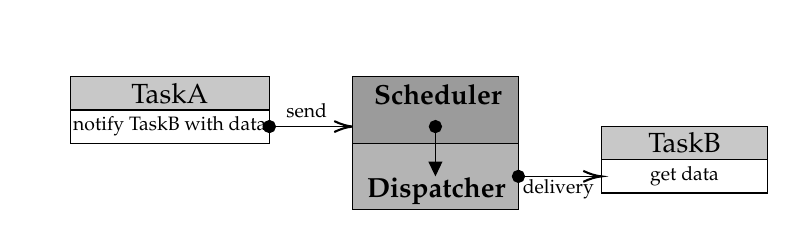
\begin{tikzpicture}[x=0.75pt,y=0.75pt,scale=0.8, yscale=-1]
\draw   (140,110) -- (260,110) -- (260,130) -- (140,130) -- cycle ;
\draw    (260,120) -- (308,120) ;
\draw [shift={(310,120)}, rotate = 180] [color={rgb, 255:red, 0; green, 0; blue, 0 }  ][line width=0.75]    (10.93,-3.29) .. controls (6.95,-1.4) and (3.31,-0.3) .. (0,0) .. controls (3.31,0.3) and (6.95,1.4) .. (10.93,3.29)   ;
\draw [shift={(260,120)}, rotate = 0] [color={rgb, 255:red, 0; green, 0; blue, 0 }  ][fill={rgb, 255:red, 0; green, 0; blue, 0 }  ][line width=0.75]      (0, 0) circle [x radius= 3.35, y radius= 3.35]   ;
\draw  [fill={rgb, 255:red, 200; green, 200; blue, 200 }  ,fill opacity=1 ] (140,90) -- (260,90) -- (260,110) -- (140,110) -- cycle ;
\draw  [fill={rgb, 255:red, 155; green, 155; blue, 155 }  ,fill opacity=1 ] (310,90) -- (410,90) -- (410,130) -- (310,130) -- cycle ;
\draw  [fill={rgb, 255:red, 180; green, 180; blue, 180 }  ,fill opacity=1 ] (310,130) -- (410,130) -- (410,170) -- (310,170) -- cycle ;
\draw    (360,120) -- (360,148) ;
\draw [shift={(360,150)}, rotate = 270] [fill={rgb, 255:red, 0; green, 0; blue, 0 }  ][line width=0.75]  [draw opacity=0] (8.93,-4.29) -- (0,0) -- (8.93,4.29) -- cycle    ;
\draw [shift={(360,120)}, rotate = 90] [color={rgb, 255:red, 0; green, 0; blue, 0 }  ][fill={rgb, 255:red, 0; green, 0; blue, 0 }  ][line width=0.75]      (0, 0) circle [x radius= 3.35, y radius= 3.35]   ;
\draw    (410,150) -- (458,150) ;
\draw [shift={(460,150)}, rotate = 180] [color={rgb, 255:red, 0; green, 0; blue, 0 }  ][line width=0.75]    (10.93,-3.29) .. controls (6.95,-1.4) and (3.31,-0.3) .. (0,0) .. controls (3.31,0.3) and (6.95,1.4) .. (10.93,3.29)   ;
\draw [shift={(410,150)}, rotate = 0] [color={rgb, 255:red, 0; green, 0; blue, 0 }  ][fill={rgb, 255:red, 0; green, 0; blue, 0 }  ][line width=0.75]      (0, 0) circle [x radius= 3.35, y radius= 3.35]   ;
\draw   (460,140) -- (560,140) -- (560,160) -- (460,160) -- cycle ;
\draw  [fill={rgb, 255:red, 200; green, 200; blue, 200 }  ,fill opacity=1 ] (460,120) -- (560,120) -- (560,140) -- (460,140) -- cycle ;
\draw (200,100) node  [align=left] {TaskA};
\draw (120,66) node  [align=left] {};
\draw (361.5,101) node  [align=left] {\textbf{Scheduler}};
% Text Node
\draw (200,120) node [scale=0.7] [align=left] {notify TaskB with data};
% Text Node
\draw (282.5,110.5) node [scale=0.7] [align=left] {send};
% Text Node
\draw (360.5,159) node  [align=left] {\textbf{Dispatcher}};
% Text Node
\draw (434,157.5) node [scale=0.7] [align=left] {delivery};
% Text Node
\draw (510,130) node  [align=left] {TaskB};
% Text Node
\draw (500,146) node  [align=left] {};
% Text Node
\draw (510,150) node [scale=0.7] [align=left] {get data};


\end{tikzpicture}


    \caption{A notification used to send an event directly from one task to another}
    \label{fig:simplenotifications}
\end{figure}




\paragraph{Simple notifications:}
Each task node has a 32-bit notification value which is initialized to zero when a task is added to the scheme. The API \lstinline{qTask_Notification_Send()} \index{\lstinline{qTask_Notification_Send}} is used to send an event directly updating the receiving task's notification value increasing it by one. As long as the scheduler sees a non-zero value, the task will be changed to a \textit{qReady} state and eventually, the dispatcher will launch the task according to the execution chain. After served, the notification value is later decreased.\\ 

\begin{lstlisting}[style=CStyle]
qBool_t qTask_Notification_Send( qTask_t * const Task, void* eventdata )
\end{lstlisting}

\subsubsection*{Parameters}
\begin{itemize}
    \item \lstinline{Task} : The pointer of the task node to which the notification is being sent 
    \item \lstinline{EventData} : Specific event user-data. 
\end{itemize}

\subsubsection*{Return value:}

\lstinline{qTrue} if the notification  has been sent, or \lstinline{qFalse} if the notification value reaches its max value. \\

\begin{tcolorbox}
\HandRight Sending simple notifications using \lstinline{qTask_Notification_Send()} is interrupt-safe, however, this only catches one event per task because the API overwrites the associated data.
\end{tcolorbox}

\paragraph{Queued notifications}
 : If the application notifies multiple events to the same task, queued notifications are the right solution instead of using simple notifications.

Here, the \lstinline{qTask_Notification_Queue()} \index{\lstinline{qTask_Notification_Queue}} take advantage of the scheduler FIFO priority-queue. 
This kind of queue, is somewhat similar to a standard queue, with an important distinction: when a notification is sent, the task is added to the queue with the corresponding priority level, and will be later removed from the queue with the highest priority task first  \cite{cormen}. That is, the tasks are (conceptually) stored in the queue in priority order instead of the insertion order. If two tasks with the same priority are notified, they are served in the FIFO form according to their order inside the queue. Figure \ref{fig:prioqueue} illustrates this behavior.

\begin{figure}[H]
    \centering
    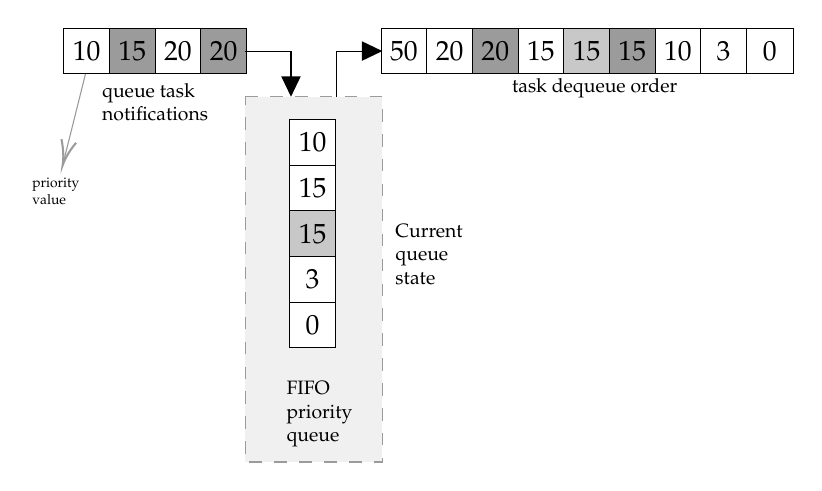
\begin{tikzpicture}[x=0.75pt,y=0.75pt,yscale=-1,xscale=1, scale=1.1]
        \draw   (100.5,50) -- (120.5,50) -- (120.5,70) -- (100.5,70) -- cycle ;
        \draw  [fill={rgb, 255:red, 155; green, 155; blue, 155 }  ,fill opacity=1 ] (120.5,50) -- (140.5,50) -- (140.5,70) -- (120.5,70) -- cycle ;
        \draw   (140.5,50) -- (160.5,50) -- (160.5,70) -- (140.5,70) -- cycle ;
        \draw  [fill={rgb, 255:red, 155; green, 155; blue, 155 }  ,fill opacity=1 ] (160.5,50) -- (180.5,50) -- (180.5,70) -- (160.5,70) -- cycle ;
        \draw   (239.5,50) -- (259.5,50) -- (259.5,70) -- (239.5,70) -- cycle ;
        \draw  [fill={rgb, 255:red, 255; green, 255; blue, 255 }  ,fill opacity=1 ] (259.5,50) -- (279.5,50) -- (279.5,70) -- (259.5,70) -- cycle ;
        \draw   (299.5,50) -- (319.5,50) -- (319.5,70) -- (299.5,70) -- cycle ;
        \draw  [fill={rgb, 255:red, 155; green, 155; blue, 155 }  ,fill opacity=1 ] (279.5,50) -- (299.5,50) -- (299.5,70) -- (279.5,70) -- cycle ;
        \draw  [color={rgb, 255:red, 155; green, 155; blue, 155 }  ,draw opacity=1 ][fill={rgb, 255:red, 240; green, 240; blue, 240 }  ,fill opacity=1 ][dash pattern={on 4.5pt off 4.5pt}] (180,80) -- (240,80) -- (240,240) -- (180,240) -- cycle ;
        \draw    (180,60) -- (200,60) -- (200,78) ;
        \draw [shift={(200,80)}, rotate = 270] [fill={rgb, 255:red, 0; green, 0; blue, 0 }  ][line width=0.75]  [draw opacity=0] (8.93,-4.29) -- (0,0) -- (8.93,4.29) -- cycle;
        \draw  [fill={rgb, 255:red, 200; green, 200; blue, 200 }  ,fill opacity=1 ] (319.5,50) -- (339.5,50) -- (339.5,70) -- (319.5,70) -- cycle ;
        \draw  [fill={rgb, 255:red, 155; green, 155; blue, 155 }  ,fill opacity=1 ] (339.5,50) -- (359.5,50) -- (359.5,70) -- (339.5,70) -- cycle ;
        \draw   (359.5,50) -- (379.5,50) -- (379.5,70) -- (359.5,70) -- cycle ;
        \draw  [fill={rgb, 255:red, 255; green, 255; blue, 255 }  ,fill opacity=1 ] (379.5,50) -- (399.5,50) -- (399.5,70) -- (379.5,70) -- cycle ;
        \draw  [fill={rgb, 255:red, 255; green, 255; blue, 255 }  ,fill opacity=1 ] (399.5,50) -- (420,50) -- (420,70) -- (399.5,70) -- cycle ;
        \draw    (220,80) -- (220,60) -- (238,60) ;
        \draw [shift={(240,60)}, rotate = 180] [fill={rgb, 255:red, 0; green, 0; blue, 0 }  ][line width=0.75]  [draw opacity=0] (8.93,-4.29) -- (0,0) -- (8.93,4.29) -- cycle;
        \draw [color={rgb, 255:red, 155; green, 155; blue, 155 }  ,draw opacity=1 ]   (110,70) -- (100.49,108.06) ;
        \draw [shift={(100,110)}, rotate = 284.04] [color={rgb, 255:red, 155; green, 155; blue, 155 }  ,draw opacity=1 ][line width=0.75]    (10.93,-3.29) .. controls (6.95,-1.4) and (3.31,-0.3) .. (0,0) .. controls (3.31,0.3) and (6.95,1.4) .. (10.93,3.29)   ;
        \draw  [fill={rgb, 255:red, 255; green, 255; blue, 255 }  ,fill opacity=1 ] (199.5,90) -- (219.5,90) -- (219.5,110) -- (199.5,110) -- cycle ;
        \draw  [fill={rgb, 255:red, 255; green, 255; blue, 255 }  ,fill opacity=1 ] (199.5,110) -- (219.5,110) -- (219.5,130) -- (199.5,130) -- cycle ;
        \draw  [fill={rgb, 255:red, 200; green, 200; blue, 200 }  ,fill opacity=1 ] (199.5,130) -- (219.5,130) -- (219.5,150) -- (199.5,150) -- cycle ;
        \draw  [fill={rgb, 255:red, 255; green, 255; blue, 255 }  ,fill opacity=1 ] (199.5,150) -- (219.5,150) -- (219.5,170) -- (199.5,170) -- cycle ;
        \draw  [fill={rgb, 255:red, 255; green, 255; blue, 255 }  ,fill opacity=1 ] (199.5,170) -- (219.5,170) -- (219.5,190) -- (199.5,190) -- cycle ;
        \draw (110.5,60) node  [align=left] {10};
        \draw (130.5,60) node  [align=left] {15};
        \draw (150.5,60) node  [align=left] {20};
        \draw (170.5,60) node  [align=left] {20};
        \draw (249.5,60) node  [align=left] {50};
        \draw (269.5,60) node  [align=left] {20};
        \draw (289.5,60) node  [align=left] {20};
        \draw (309.5,60) node  [align=left] {15};
        \draw (369.5,60) node  [align=left] {10};
        \draw (329.5,60) node  [align=left] {15};
        \draw (349.5,60) node  [align=left] {15};
        \draw (389.5,60) node  [align=left] {3};
        \draw (409.75,60) node  [align=left] {0};
        \draw (260.5,149) node [scale=0.7] [align=left] {Current\\queue\\state};
        \draw (333,76.5) node [scale=0.7] [align=left] {task dequeue order};
        \draw (140.5,82.5) node [scale=0.7] [align=left] {queue task \\notifications};
        \draw (97,121.5) node [scale=0.5] [align=left] {priority\\value};
        \draw (209.5,100) node  [align=left] {10};
        \draw (209.5,120) node  [align=left] {15};
        \draw (209.5,140) node  [align=left] {15};
        \draw (209.5,160) node  [align=left] {3};
        \draw (209.5,180) node  [align=left] {0};
        \draw (212.5,219) node [scale=0.7] [align=left] {FIFO\\priority\\queue};
    \end{tikzpicture}
    \caption{Priority-queue behavior}
    \label{fig:prioqueue}
\end{figure}

The scheduler always checks the queue state first, being this event the one with more precedence among the others. If the queue has elements, the scheduler algorithm will extract the data and the corresponding task will be launched with the trigger flag set in \textit{byNotificationQueued}. \\

\begin{lstlisting}[style=CStyle]
qBool_t qTask_Notification_Queue( qTask_t * const Task, void* eventdata )
\end{lstlisting}

\subsubsection*{Parameters}
\begin{itemize}
    \item \lstinline{Task} : The pointer of the task node to which the notification is being sent 
    \item \lstinline{EventData} : Specific event user-data. 
\end{itemize}

\subsubsection*{Return value:}

\lstinline{qTrue} if the notification  has been inserted in the queue, or \lstinline{qFalse} if an error occurred or the queue exceeds the size. \\

\begin{tcolorbox}
\HandRight Among all the provided events, queued notifications have the highest precedence.
\end{tcolorbox}


Figure ~\ref{fig:queueexample}, shows a cooperative environment with five tasks. Initially, the scheduler activates \lstinline{Task-E}, then, this task enqueues data to \lstinline{Task-A} and \lstinline{Task-B} respectively using the \lstinline{qTask_Notification_Queue()} function. In the next scheduler cycle, the scheduler realizes that the priority-queue is not empty, generating an activation over the task located at the beginning of the queue. In this case, \lstinline{Task-A} will be launched and its respective data will be extracted from the queue. However, \lstinline{Task-A} also enqueues data to \lstinline{Task-C} and \lstinline{Task-D}. As mentioned previously, this is a priority-queue, so the scheduler makes a new reordering. In this context, the next queue extraction will be for \lstinline{Task-D}, \lstinline{Task-C}, and \lstinline{Task-B} sequentially.

\begin{figure}[H]
    \centering
    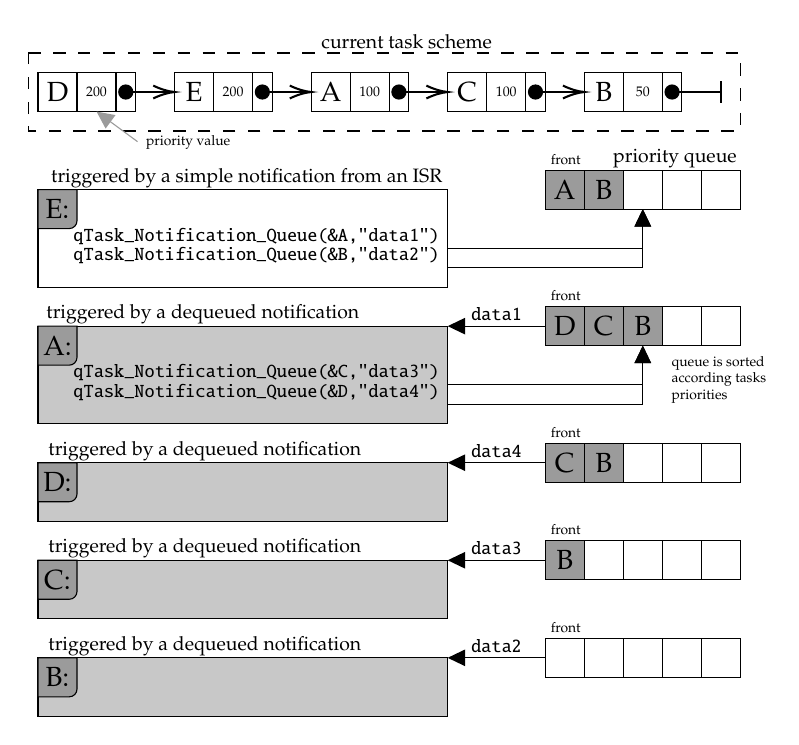
\begin{tikzpicture}[x=0.75pt,y=0.75pt,yscale=-1,xscale=1,scale=0.94]
        \draw  [fill={rgb, 255:red, 155; green, 155; blue, 155 }  ,fill opacity=1 ] (360,110) -- (380,110) -- (380,130) -- (360,130) -- cycle ;
        \draw  [fill={rgb, 255:red, 155; green, 155; blue, 155 }  ,fill opacity=1 ] (380,110) -- (400,110) -- (400,130) -- (380,130) -- cycle ;
        \draw   (400,110) -- (420,110) -- (420,130) -- (400,130) -- cycle ;
        \draw   (420,110) -- (440,110) -- (440,130) -- (420,130) -- cycle ;
        \draw   (440,110) -- (460,110) -- (460,130) -- (440,130) -- cycle ;
        \draw   (100,120) -- (310,120) -- (310,170) -- (100,170) -- cycle ;
        \draw  [fill={rgb, 255:red, 155; green, 155; blue, 155 }  ,fill opacity=1 ] (120,136) .. controls (120,138.21) and (118.21,140) .. (116,140) -- (100,140) -- (100,120) -- (120,120) -- cycle ;
        \draw  [fill={rgb, 255:red, 155; green, 155; blue, 155 }  ,fill opacity=1 ] (360,180) -- (380,180) -- (380,200) -- (360,200) -- cycle ;
        \draw  [fill={rgb, 255:red, 155; green, 155; blue, 155 }  ,fill opacity=1 ] (380,180) -- (400,180) -- (400,200) -- (380,200) -- cycle ;
        \draw  [fill={rgb, 255:red, 155; green, 155; blue, 155 }  ,fill opacity=1 ] (400,180) -- (420,180) -- (420,200) -- (400,200) -- cycle ;
        \draw   (420,180) -- (440,180) -- (440,200) -- (420,200) -- cycle ;
        \draw   (440,180) -- (460,180) -- (460,200) -- (440,200) -- cycle ;
        \draw  [fill={rgb, 255:red, 200; green, 200; blue, 200 }  ,fill opacity=1 ] (100,190) -- (310,190) -- (310,240) -- (100,240) -- cycle ;
        \draw  [fill={rgb, 255:red, 155; green, 155; blue, 155 }  ,fill opacity=1 ] (120,206) .. controls (120,208.21) and (118.21,210) .. (116,210) -- (100,210) -- (100,190) -- (120,190) -- cycle ;
        \draw  [fill={rgb, 255:red, 200; green, 200; blue, 200 }  ,fill opacity=1 ] (100,260) -- (310,260) -- (310,290) -- (100,290) -- cycle ;
        \draw  [fill={rgb, 255:red, 155; green, 155; blue, 155 }  ,fill opacity=1 ] (120,276) .. controls (120,278.21) and (118.21,280) .. (116,280) -- (100,280) -- (100,260) -- (120,260) -- cycle ;
        \draw  [fill={rgb, 255:red, 200; green, 200; blue, 200 }  ,fill opacity=1 ] (100,310) -- (310,310) -- (310,340) -- (100,340) -- cycle ;
        \draw  [fill={rgb, 255:red, 155; green, 155; blue, 155 }  ,fill opacity=1 ] (120,326) .. controls (120,328.21) and (118.21,330) .. (116,330) -- (100,330) -- (100,310) -- (120,310) -- cycle ;
        \draw  [fill={rgb, 255:red, 200; green, 200; blue, 200 }  ,fill opacity=1 ] (100,360) -- (310,360) -- (310,390) -- (100,390) -- cycle ;
        \draw  [fill={rgb, 255:red, 155; green, 155; blue, 155 }  ,fill opacity=1 ] (120,376) .. controls (120,378.21) and (118.21,380) .. (116,380) -- (100,380) -- (100,360) -- (120,360) -- cycle ;
        \draw  [fill={rgb, 255:red, 155; green, 155; blue, 155 }  ,fill opacity=1 ] (360,250) -- (380,250) -- (380,270) -- (360,270) -- cycle ;
        \draw  [fill={rgb, 255:red, 155; green, 155; blue, 155 }  ,fill opacity=1 ] (380,250) -- (400,250) -- (400,270) -- (380,270) -- cycle ;
        \draw   (400,250) -- (420,250) -- (420,270) -- (400,270) -- cycle ;
        \draw   (420,250) -- (440,250) -- (440,270) -- (420,270) -- cycle ;
        \draw   (440,250) -- (460,250) -- (460,270) -- (440,270) -- cycle ;
        \draw  [fill={rgb, 255:red, 155; green, 155; blue, 155 }  ,fill opacity=1 ] (360,300) -- (380,300) -- (380,320) -- (360,320) -- cycle ;
        \draw   (380,300) -- (400,300) -- (400,320) -- (380,320) -- cycle ;
        \draw   (400,300) -- (420,300) -- (420,320) -- (400,320) -- cycle ;
        \draw   (420,300) -- (440,300) -- (440,320) -- (420,320) -- cycle ;
        \draw   (440,300) -- (460,300) -- (460,320) -- (440,320) -- cycle ;
        \draw   (360,350) -- (380,350) -- (380,370) -- (360,370) -- cycle ;
        \draw   (380,350) -- (400,350) -- (400,370) -- (380,370) -- cycle ;
        \draw   (400,350) -- (420,350) -- (420,370) -- (400,370) -- cycle ;
        \draw   (420,350) -- (440,350) -- (440,370) -- (420,370) -- cycle ;
        \draw   (440,350) -- (460,350) -- (460,370) -- (440,370) -- cycle ;
        \draw    (360,190) -- (312,190) ;
        \draw [shift={(310,190)}, rotate = 360] [fill={rgb, 255:red, 0; green, 0; blue, 0 }  ][line width=0.75]  [draw opacity=0] (8.93,-4.29) -- (0,0) -- (8.93,4.29) -- cycle;
        \draw    (360,260) -- (312,260) ;
        \draw [shift={(310,260)}, rotate = 360] [fill={rgb, 255:red, 0; green, 0; blue, 0 }  ][line width=0.75]  [draw opacity=0] (8.93,-4.29) -- (0,0) -- (8.93,4.29) -- cycle;
        \draw    (360,310) -- (312,310) ;
        \draw [shift={(310,310)}, rotate = 360] [fill={rgb, 255:red, 0; green, 0; blue, 0 }  ][line width=0.75]  [draw opacity=0] (8.93,-4.29) -- (0,0) -- (8.93,4.29) -- cycle;
        \draw    (360,360) -- (312,360) ;
        \draw [shift={(310,360)}, rotate = 360] [fill={rgb, 255:red, 0; green, 0; blue, 0 }  ][line width=0.75]  [draw opacity=0] (8.93,-4.29) -- (0,0) -- (8.93,4.29) -- cycle;
        \draw    (310,150) -- (410,150) -- (410,132) ;
        \draw [shift={(410,130)}, rotate = 450] [fill={rgb, 255:red, 0; green, 0; blue, 0 }  ][line width=0.75]  [draw opacity=0] (8.93,-4.29) -- (0,0) -- (8.93,4.29) -- cycle;
        \draw    (310,160) -- (410,160) -- (410,132) ;
        \draw [shift={(410,130)}, rotate = 450] [fill={rgb, 255:red, 0; green, 0; blue, 0 }  ][line width=0.75]  [draw opacity=0] (8.93,-4.29) -- (0,0) -- (8.93,4.29) -- cycle;
        \draw    (310,220) -- (410,220) -- (410,202) ;
        \draw [shift={(410,200)}, rotate = 450] [fill={rgb, 255:red, 0; green, 0; blue, 0 }  ][line width=0.75]  [draw opacity=0] (8.93,-4.29) -- (0,0) -- (8.93,4.29) -- cycle;
        \draw    (310,230) -- (410,230) -- (410,202) ;
        \draw [shift={(410,200)}, rotate = 450] [fill={rgb, 255:red, 0; green, 0; blue, 0 }  ][line width=0.75]  [draw opacity=0] (8.93,-4.29) -- (0,0) -- (8.93,4.29) -- cycle;
        \draw   (100,60) -- (120,60) -- (120,80) -- (100,80) -- cycle ;
        \draw   (120,60) -- (140,60) -- (140,80) -- (120,80) -- cycle ;
        \draw   (140,60) -- (150,60) -- (150,80) -- (140,80) -- cycle ;
        \draw   (170,60) -- (190,60) -- (190,80) -- (170,80) -- cycle ;
        \draw   (190,60) -- (210,60) -- (210,80) -- (190,80) -- cycle ;
        \draw   (210,60) -- (220,60) -- (220,80) -- (210,80) -- cycle ;
        \draw   (240,60) -- (260,60) -- (260,80) -- (240,80) -- cycle ;
        \draw   (260,60) -- (280,60) -- (280,80) -- (260,80) -- cycle ;
        \draw   (280,60) -- (290,60) -- (290,80) -- (280,80) -- cycle ;
        \draw   (310,60) -- (330,60) -- (330,80) -- (310,80) -- cycle ;
        \draw   (330,60) -- (350,60) -- (350,80) -- (330,80) -- cycle ;
        \draw   (350,60) -- (360,60) -- (360,80) -- (350,80) -- cycle ;\draw   (380,60) -- (400,60) -- (400,80) -- (380,80) -- cycle ;
        \draw   (400,60) -- (420,60) -- (420,80) -- (400,80) -- cycle ;
        \draw   (420,60) -- (430,60) -- (430,80) -- (420,80) -- cycle ;
        \draw    (145,70) -- (168,70) ;
        \draw [shift={(170,70)}, rotate = 180] [color={rgb, 255:red, 0; green, 0; blue, 0 }  ][line width=0.75]    (10.93,-3.29) .. controls (6.95,-1.4) and (3.31,-0.3) .. (0,0) .. controls (3.31,0.3) and (6.95,1.4) .. (10.93,3.29)   ;
        \draw [shift={(145,70)}, rotate = 0] [color={rgb, 255:red, 0; green, 0; blue, 0 }  ][fill={rgb, 255:red, 0; green, 0; blue, 0 }  ][line width=0.75]      (0, 0) circle [x radius= 3.35, y radius= 3.35]   ;
        \draw    (215,70) -- (238,70) ;
        \draw [shift={(240,70)}, rotate = 180] [color={rgb, 255:red, 0; green, 0; blue, 0 }  ][line width=0.75]    (10.93,-3.29) .. controls (6.95,-1.4) and (3.31,-0.3) .. (0,0) .. controls (3.31,0.3) and (6.95,1.4) .. (10.93,3.29)   ;
        \draw [shift={(215,70)}, rotate = 0] [color={rgb, 255:red, 0; green, 0; blue, 0 }  ][fill={rgb, 255:red, 0; green, 0; blue, 0 }  ][line width=0.75]      (0, 0) circle [x radius= 3.35, y radius= 3.35]   ;
        \draw    (285,70) -- (308,70) ;
        \draw [shift={(310,70)}, rotate = 180] [color={rgb, 255:red, 0; green, 0; blue, 0 }  ][line width=0.75]    (10.93,-3.29) .. controls (6.95,-1.4) and (3.31,-0.3) .. (0,0) .. controls (3.31,0.3) and (6.95,1.4) .. (10.93,3.29)   ;
        \draw [shift={(285,70)}, rotate = 0] [color={rgb, 255:red, 0; green, 0; blue, 0 }  ][fill={rgb, 255:red, 0; green, 0; blue, 0 }  ][line width=0.75]      (0, 0) circle [x radius= 3.35, y radius= 3.35]   ;
        \draw    (355,70) -- (378,70) ;
        \draw [shift={(380,70)}, rotate = 180] [color={rgb, 255:red, 0; green, 0; blue, 0 }  ][line width=0.75]    (10.93,-3.29) .. controls (6.95,-1.4) and (3.31,-0.3) .. (0,0) .. controls (3.31,0.3) and (6.95,1.4) .. (10.93,3.29)   ;
        \draw [shift={(355,70)}, rotate = 0] [color={rgb, 255:red, 0; green, 0; blue, 0 }  ][fill={rgb, 255:red, 0; green, 0; blue, 0 }  ][line width=0.75]      (0, 0) circle [x radius= 3.35, y radius= 3.35]   ;
        \draw    (425,70) -- (450,70) ;
        \draw [shift={(450,70)}, rotate = 180] [color={rgb, 255:red, 0; green, 0; blue, 0 }  ][line width=0.75]    (0,5.59) -- (0,-5.59)   ;
        \draw [shift={(425,70)}, rotate = 0] [color={rgb, 255:red, 0; green, 0; blue, 0 }  ][fill={rgb, 255:red, 0; green, 0; blue, 0 }  ][line width=0.75]      (0, 0) circle [x radius= 3.35, y radius= 3.35]   ;
        \draw  [dash pattern={on 4.5pt off 4.5pt}] (95,50) -- (460,50) -- (460,90) -- (95,90) -- cycle ;
        \draw [color={rgb, 255:red, 155; green, 155; blue, 155 }  ,draw opacity=1 ]   (151.02,95.44) -- (131.61,81.18) ;
        \draw [shift={(130,80)}, rotate = 396.31] [fill={rgb, 255:red, 155; green, 155; blue, 155 }  ,fill opacity=1 ][line width=0.75]  [draw opacity=0] (8.93,-4.29) -- (0,0) -- (8.93,4.29) -- cycle    ;
        \draw (212,154) node [scale=0.7] [align=left] {\ttfamily{qTask_Notification_Queue(\&B,"data2")}};
        \draw (212,144) node [scale=0.7] [align=left] {\ttfamily{qTask_Notification_Queue(\&A,"data1")}};
        \draw (110,130) node  [align=left] {E:};
        \draw (212,224) node [scale=0.7] [align=left] {\ttfamily{qTask_Notification_Queue(\&D,"data4")}};
        \draw (212,214) node [scale=0.7] [align=left] {\ttfamily{qTask_Notification_Queue(\&C,"data3")}};
        \draw (110,200) node  [align=left] {A:};
        \draw (110,270) node  [align=left] {D:};
        \draw (184.5,184) node [scale=0.7] [align=left] {triggered by a dequeued notification};
        \draw (185.5,254) node [scale=0.7] [align=left] {triggered by a dequeued notification};
        \draw (110,320) node  [align=left] {C:};
        \draw (185.5,304) node [scale=0.7] [align=left] {triggered by a dequeued notification};
        \draw (110,370) node  [align=left] {B:};
        \draw (185.5,354) node [scale=0.7] [align=left] {triggered by a dequeued notification};
        \draw (370.5,104.5) node [scale=0.5] [align=left] {front};
        \draw (370.5,174.5) node [scale=0.5] [align=left] {front};
        \draw (370.5,244.5) node [scale=0.5] [align=left] {front};
        \draw (370.5,294.5) node [scale=0.5] [align=left] {front};
        \draw (370.5,344.5) node [scale=0.5] [align=left] {front};
        \draw (370,120) node  [align=left] {A};
        \draw (390,120) node  [align=left] {B};
        \draw (370,190) node  [align=left] {D};
        \draw (390,190) node  [align=left] {C};
        \draw (410,190) node  [align=left] {B};
        \draw (370,260) node  [align=left] {C};
        \draw (390,260) node  [align=left] {B};
        \draw (370,310) node  [align=left] {B};
        \draw (335,184) node [scale=0.7] [align=left] {\ttfamily{data1}};
        \draw (335,254) node [scale=0.7] [align=left] {\ttfamily{data4}};
        \draw (335,304) node [scale=0.7] [align=left] {\ttfamily{data3}};
        \draw (335,354) node [scale=0.7] [align=left] {\ttfamily{data2}};
        \draw (207,114) node [scale=0.7] [align=left] {triggered by a simple notification from an ISR};
        \draw (110,70) node  [align=left] {D};
        \draw (180,70) node  [align=left] {E};
        \draw (250,70) node  [align=left] {A};
        \draw (320,70) node  [align=left] {C};
        \draw (390,70) node  [align=left] {B};
        \draw (130,70) node [scale=0.5] [align=left] {200};
        \draw (200,70) node [scale=0.5] [align=left] {200};
        \draw (270,70) node [scale=0.5] [align=left] {100};
        \draw (340,70) node [scale=0.5] [align=left] {100};
        \draw (410,70) node [scale=0.5] [align=left] {50};
        \draw (289,44) node [scale=0.7] [align=left] {current task scheme};
        \draw (177,96) node [scale=0.5,color={rgb, 255:red, 0; green, 0; blue, 0 }  ,opacity=1 ] [align=left] {priority value};
        \draw (426.5,104) node [scale=0.7] [align=left] {priority queue};
        \draw (449,217.5) node [scale=0.5] [align=left] {queue is sorted \\according tasks \\priorities};
    \end{tikzpicture}
    \caption{Priority-queue example}
    \label{fig:queueexample}
\end{figure}

\begin{tcolorbox}
\HandRight Any queue extraction involves an activation to the receiving task. The extracted data will be available inside the \lstinline{qEvent_t} structure.
\end{tcolorbox}

\subsubsection{Spread a notification}
In some systems, we need the ability to broadcast an event to all tasks. This is often referred to as a \textit{barrier}. This means that a group of tasks should stop activities at some point and cannot proceed until another task or ISR raise a specific event. 
For this kind of implementations, the \lstinline{qOS_Notification_Spread()} \index{\lstinline{qOS_Notification_Spread}} can be used. \\

\begin{lstlisting}[style=CStyle]
qBool_t qOS_Notification_Spread( const void *eventdata, 
                                 const qTask_NotifyMode_t mode )
\end{lstlisting}

\subsubsection*{Parameters}
\begin{itemize}
    \item \lstinline{eventdata} : Specific event user-data. 
    \item \lstinline{mode} : The method used to spread the event: \lstinline{Q_NOTIFY_SIMPLE} or \lstinline{Q_NOTIFY_QUEUED}
\end{itemize}

\subsubsection*{Return value:}

\lstinline{qTrue} on success. Otherwise \lstinline{qFalse}.

\noindent\hrulefill
\newline

\begin{tcolorbox}
\HandRight This function spreads a notification event among all the tasks in the scheduling scheme, so,  for tasks that are not part of the barrier, just discard the notification. This operation will be performed in the next scheduling cycle.
\end{tcolorbox}

\subsubsection{Queues}
A queue is a linear data structure with simple operations based on the FIFO (First In First Out) principle. It is capable to hold a finite number of fixed-size data items. The maximum number of items that a queue can hold is called its \textit{length}. Both the length and the size of each data item are set when the queue is created.

\begin{figure}[H]
    \centering
    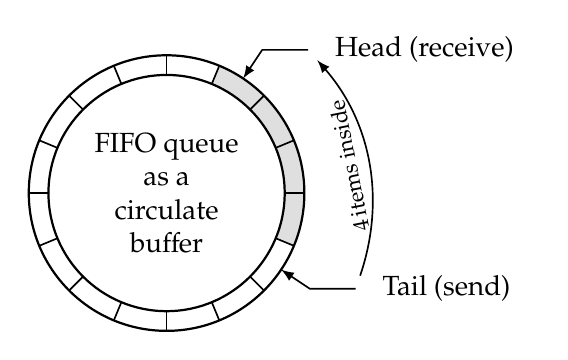
\begin{tikzpicture}[>=latex,semithick,scale=1.75]
        \fill [gray!25] (0,0) -- (67.5:1) arc [end angle=-22.5, start angle=67.5, radius=1] -- cycle;
        \draw [thick] (0,0) circle (1);
        \foreach \angle in {90,67.5,...,-67.5}
            \draw (\angle:1) -- (\angle-180:1);
        \node [circle,thick,fill=white,draw=black,align=center,minimum size=3cm] at (0,0) {FIFO queue\\ as a\\circulate \\buffer};
        \draw [<-] (56.25:1) -- (56.25:1.25) -- +(.333,0)
            node [right,inner xsep=.333cm] (Head) {Head (receive)};
        \draw [<-] (-33.75:1) -- (-33.75:1.25) -- +(.333,0)
            node [right,inner xsep=.333cm] (Tail) {Tail (send)};
        \draw [->,shorten >=5pt,shorten <=5pt] (Tail.west) to [bend right] 
            node [midway,sloped,above,allow upside down] {\footnotesize 4\,items inside}
        (Head.west);
    \end{tikzpicture}
    \caption{qQueues conceptual representation}
    \label{fig:qqueues}
\end{figure}

As showed in figure \ref{fig:qqueues}, the last position is connected back to the first position to make a circle. It is also called \textit{ring-buffer} or \textit{circular-queue}. 

In general, this kind of data structure is used to serialize data between tasks, allowing some elasticity in time. In many cases, the queue is used as a data buffer in interrupt service routines. This buffer will collect the data so, at some later time, another task can fetch the data for further processing. This use case is the single "task to task" buffering case. There are also other applications for queues as serializing  many data streams into one receiving streams (multiple tasks to a single task) or vice-versa (single task to multiple tasks).
The usage of this data structure is detailed in section \ref{queuecreate}. \\

\begin{tcolorbox}
\ArrowBoldDownRight Note : The OS uses the queue by copy method. Queuing by copy is considered to be simultaneously more powerful and simpler to use than queuing by reference.
\end{tcolorbox}

Queuing by copy does not prevent the queue from also being used to queue by reference. For example, when the size of the data being queued makes it impractical to copy the data into the queue, then a pointer to the data can be copied into the queue instead.

\subsubsection{Event Flags}
Every task node has a set of built-in event bits called \textit{Event-Flags}, that can be used to indicate if an event has occurred or not.  
They are somewhat similar to signals, but with greater flexibility, providing a low cost, but flexible means of passing simple messages between tasks. One task can set or clear any combination of event flags. Another task may read the event flag group at any time or may wait for a specific pattern of flags.  
\begin{figure}[H]
    \centering
    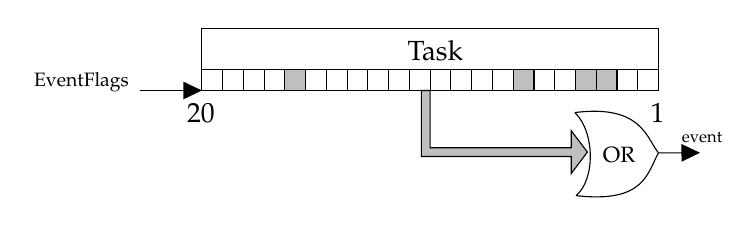
\begin{tikzpicture}[x=0.75pt,y=0.75pt,yscale=-1,xscale=1]
        \foreach \x in {100,110,...,270}{
            \draw   (\x,120) -- (\x+10,120) -- (\x+10,130) -- (\x,130) -- cycle ;
        }
        \draw  [fill=gray!50  ,fill opacity=1 ] (140,120) -- (150,120) -- (150,130) -- (140,130) -- cycle ;
        \draw  [fill=gray!50  ,fill opacity=1 ] (250,120) -- (260,120) -- (260,130) -- (250,130) -- cycle ;
        \draw  [fill=gray!50  ,fill opacity=1 ] (280,120) -- (290,120) -- (290,130) -- (280,130) -- cycle ;
        \draw  [fill=gray!50  ,fill opacity=1 ] (290,120) -- (300,120) -- (300,130) -- (290,130) -- cycle ;
        \draw   (300,120) -- (310,120) -- (310,130) -- (300,130) -- cycle ;
        \draw   (310,120) -- (320,120) -- (320,130) -- (310,130) -- cycle ;
        \draw   (100,100) -- (320,100) -- (320,120) -- (100,120) -- cycle ;
        \draw    (70,130) -- (79.5,130) -- (98,130) ;
        \draw [shift={(100,130)}, rotate = 180] [fill=black  ][line width=0.75]  [draw opacity=0] (8.93,-4.29) -- (0,0) -- (8.93,4.29) -- cycle    ;
        \draw    (320,160.06) .. controls (314.64,169.47) and (313.5,184.5) .. (280.29,180.64) ;
        \draw    (320,160.06) .. controls (314.4,153.47) and (312.16,136.5) .. (279.71,140.64) ;
        \draw    (280.29,180.64) .. controls (289.68,172.83) and (289.35,149.84) .. (279.71,140.64) ;
        \draw  [fill=gray!50  ,fill opacity=1 ] (210,130) -- (210,157.56) -- (277.94,157.56) -- (277.94,149.36) -- (285.75,159.68) -- (277.94,170) -- (277.94,161.8) -- (205.75,161.8) -- (205.75,130) -- cycle ;
        \draw    (320,160.06) -- (329.5,160.06) -- (338,160.01) ;
        \draw [shift={(340,160)}, rotate = 539.67] [fill=black ][line width=0.75]  [draw opacity=0] (8.93,-4.29) -- (0,0) -- (8.93,4.29) -- cycle    ;
        \draw (99.5,141) node  [align=left] {20};
        \draw (319.5,141) node  [align=left] {1};
        \draw (212.5,111) node  [align=left] {Task};
        \draw (42,126) node [scale=0.7] [align=left] {EventFlags};
        \draw (301,161) node [scale=0.8] [align=left] {OR};
        \draw (341,152.5) node [scale=0.6] [align=left] {event};
    \end{tikzpicture}
    \caption{Task event flags}
    \label{fig:eventflags}
\end{figure}

Up to twenty(20) bit-flags are available per task and whenever the scheduler sees that one event-flag is set, the kernel will trigger the task execution.
\\
The function \lstinline{qTask_EventFlags_Modify} is intended to modify the task event-flags: \\

\begin{lstlisting}[style=CStyle]
void qTask_EventFlags_Modify( qTask_t * const Task, qTaskFlag_t flags, 
                              qBool_t action )
\end{lstlisting} \index{\lstinline{qTask_EventFlags_Modify}}

\subsubsection*{Parameters}
\begin{itemize}
    \item \lstinline{Task} : A pointer to the task node.
    \item \lstinline{flags} : The flags to modify. Can be combined with a bitwise \lstinline{OR} (\lstinline{|}).
    
    \lstinline{ QEVENTFLAG_01 | QEVENTFLAG_02 | QEVENTFLAG_03 | ... | QEVENTFLAG_20 }
    \item \lstinline{action} : \lstinline{QEVENTFLAG_SET} or \lstinline{QEVENTFLAG_CLEAR}. 
\end{itemize}
\newline

\begin{tcolorbox}
\HandRight The scheduler will put the task into a \textit{qReady} state when any of the available event-flags is set. The flags should be cleared by the application writer explicitly. 
\end{tcolorbox}
\newline
To read or check the event flags, the application can use one of the following API functions: \\

\begin{lstlisting}[style=CStyle]
qTaskFlag_t qTask_EventFlags_Read( const qTask_t * const Task )
\end{lstlisting} \index{\lstinline{qTask_EventFlags_Read}}

\subsubsection*{Parameters}
\begin{itemize}
    \item \lstinline{Task} : A pointer to the task node.
\end{itemize}

\subsubsection*{Return value:}

The EventFlag value of the task.

\noindent\hrulefill
\newline


\begin{lstlisting}[style=CStyle]
qBool_t qTask_EventFlags_Check( qTask_t * const Task, 
                                qTaskFlag_t FlagsToCheck, 
                                qBool_t ClearOnExit, 
                                qBool_t CheckForAll )
\end{lstlisting} \index{\lstinline{qTask_EventFlags_Check}}

\subsubsection*{Parameters}
\begin{itemize}
    \item \lstinline{Task} : A pointer to the task node.
    \item \lstinline{FlagsToCheck} : A bitwise value that indicates the flags to test inside the EventFlags. Can be combined with a bitwise ‘OR’ (\lstinline{'|'}).
    \item \lstinline{ClearOnExit} : If is set to \lstinline{qTrue} then any flags set in the value passed as the \lstinline{FlagsToCheck} parameter will be cleared in the event group before this function returns only when the condition is meet.
    \item \lstinline{CheckForAll} : Used to create either a logical AND test (where all flags must be set)or a logical OR test (where one or more flags must be set) as follows:
    
    If is set to \lstinline{qTrue} this API will return \lstinline{qTrue} when all the flags set in the value passed as the \lstinline{FlagsToCheck} parameter are set in the task's EventFlags.
    
    If is set to \lstinline{qFalse} this API will return \lstinline{qTrue} when any of the flags set in the value passed as the \lstinline{FlagsToCheck} parameter are set in the task's EventFlags.

\end{itemize}

\subsubsection*{Return value:}

\lstinline{qTrue} if the condition is meet, otherwise return \lstinline{qFalse}.


\subsection{Retrieving the event data} \label{eventdata} \index{\lstinline{qEvent_t}}
As you can read in the previous sections, tasks can be triggered from multiple event sources (time-elapsed, notifications, queues and event-flags). This can lead to several situations that must be handled by the application writer from the task context, for example:

\begin{itemize}
    \item What is the event source that triggers the task execution?
    \item How to get the event associated data?
    \item What is the task execution status? 
\end{itemize}

The OS provides a simple approach for this, a data structure with all the regarding information of the task execution. This structure, that is already defined in the callback function as the \lstinline{qEvent_t} argument, is filled by the kernel dispatcher, so the application writer only needs to read the fields inside.

This data structure is defined as: \\

\begin{lstlisting}[style=CStyle]
typedef struct{
    qTrigger_t Trigger;
    void *TaskData;
    void *EventData;
    qBool_t FirstCall, FirstIteration, LastIteration;
}qEvent_t;
\end{lstlisting}

Each field of the structure is described as follows
\begin{itemize}
    \item \lstinline{Trigger} : The flag that indicates the event source that triggers the task execution. This flag can only have nine(9) possible values:
    \begin{itemize}
        \item \lstinline{byTimeElapsed}  : When the time specified for the task elapsed.
        \item \lstinline{byNotificationQueued} : When there is a queued notification in the FIFO priority queue. For this trigger, the dispatcher performs a dequeue operation automatically. A pointer to the dequeued event-data will be available in the \lstinline{EventData}  field.
        \item \lstinline{byNotificationSimple} : When an asynchronous notification event  arrives by the usage of \lstinline{qTask_Notification_Send}. A pointer to the notification data will be available in the \lstinline{EventData} field.
        \item \lstinline{byQueueReceiver} : When there are elements available in the attached queue, the scheduler makes a data dequeue(auto-receive) from the front. A pointer to the received data will be available in the \lstinline{EventData} field.
        \item \lstinline{byQueueFull} : When the attached queue is full. A pointer to the queue will be available in the \lstinline{EventData} field.
        \item \lstinline{byQueueCount} : When the element-count of the  attached queue reaches
        the specified value. A pointer to the queue will be available in the \lstinline{EventData} field.
        \item \lstinline{byQueueEmpty} : When the attached queue is empty. A pointer to the queue will be available in the \lstinline{EventData} field.
        \item \lstinline{byEventFlags} : When any of the available event flags is set. Flags should be cleared by the application writer.
        \item \lstinline{byNoReadyTasks} : Only when the idle task is triggered
    \end{itemize}
    \item \lstinline{TaskData} : The storage pointer. Tasks can store a pointer to specific variable, structure or array, which represents specific user data for a particular task. This may be needed if you plan to use the same callback method for multiple tasks.
    \item \lstinline{EventData} : Associated data of the event. Specific data will reside here according to the event source. This field will have a \lstinline{NULL} value when the trigger gets one of this values:  \textit{byTimeElapsed}, \textit{byEventFlags} and \textit{byNoReadyTasks}.
    \item \lstinline{FirstCall} : This flag indicates that a task is running for the first time. Can be used for data initialization purposes.
    \item \lstinline{FirstIteration} : Indicates whether current pass is the first iteration of the task. This flag will be only set when time-elapsed events occurs and the iteration counter has been parameterized. 
    \item \lstinline{LastIteration} : Indicates whether current pass is the last iteration of the task. This flag will be only set when time-elapsed events occurs and the iteration counter has been parameterized. 
    \item \lstinline{StartDelay} : The number of epochs between current system time and point in time when the task was marked as Ready.
    Can be used to keep track when current task's execution took place relative to when it was scheduled. A value of 0 (zero) indicates that task started right on time per schedule.
    This parameter will be only available on timed tasks, when \lstinline{Trigger} \lstinline{==} \textit{byTimeElapsed}. 
\end{itemize}    

\begin{tcolorbox}
\HandRight Asynchronous events never change the task iteration counter, consequently, it has no effect on related fields, \lstinline{FirstIteration} and \lstinline{LastIteration}.
\end{tcolorbox}
    
\subsection{Implementation guidelines}
\subsubsection{Sending notifications}

The kernel handles all the notifications by itself (simple or queued), so intermediate objects aren't needed. Just calling \lstinline{qTask_Notification_Send()} or \lstinline{qTask_Notification_Queue()} is enough to send notifications. After the task callback is invoked, the notification is cleared by the dispatcher. Here the application writer must read the respective fields of the event-data structure to check the received notification. \\

The next example shows an ISR to task communication. Two interrupts send notifications to a single task with specific event data. The receiver task (\lstinline{taskA}) after further processing, send an event to \lstinline{taskB} to handle the event generated by the transmitter (\lstinline{taskA}).

\begin{lstlisting}[style=CStyle]
#include <stdio.h>
#include <stdlib.h>
#include <string.h>
#include "HAL.h" /*hardware dependent code*/
#include "QuarkTS.h"

qTask_t taskA, taskB;
void taskA_Callback( qEvent_t e );
void taskB_Callback( qEvent_t e );

const char *app_events[] = {
                            "Timer1seg", 
                            "ButtonRisingEdge", 
                            "ButtonFallingEdge", 
                            "3Count_ButtonPush"
                            };

/*==================================================================*/
void interrupt Timer1Second_ISR( void) {
    qTask_Notification_Send( &taskA, NULL );
    HAL_ClearInterruptFlags( HAL_TMR_ISR ); /*hardware dependent code*/
}
/*==================================================================*/
void interrupt ExternalInput_ISR( void ){
    if( RISING_EDGE == HAL_GetInputEdge() ){ /*hardware dependent code*/
        qTask_Notification_Queue( &taskA, app_events[1] );    
    }
    else{
        qTask_Notification_Queue( &taskA, app_events[2] );
    }
    HAL_ClearInterruptFlags( HAL_EXT_ISR ); /*hardware dependent code*/
}
/*==================================================================*/
void taskA_Callback( qEvent_t e ){
    static int press_counter = 0;
    
    switch(e->Trigger){ /*check the source of the event*/
        case byNotificationSimple: 
            /*
            * Do something here to process the timer event
            */
            break;
        case byNotificationQueued:
            /*here, we only care the Falling Edge events*/
            if( strcmp( e->EventData, "ButtonFallingEdge" )==0 ){
                press_counter++; /*count the button press*/
                if( press_counter == 3){ /*after 3 presses*/
                    /*send the notification of 3 presses to taskB*/
                    qTask_Notification_Send( &taskB, app_events[3] );
                    press_counter = 0;
                }
            }
            break;
        default:
            break;
    }
}
/*==================================================================*/
void taskB_Callback( qEvent_t e ){
    if( byNotificationSimple == e->Trigger){
        /*
         * we can do more here, but this is just an example,
         * so, this task will only print out the received 
         * notification event.
         */
        qDebug( e->EventData, Message );
    }
}
/*==================================================================*/
int main( void ){
    HAL_Setup_MCU(); /*hardware dependent code*/
    qTrace_Set_OutputFcn( HAL_OutPutChar );
    /* setup the scheduler to handle up to 10 queued notifications*/
    qOS_Setup( HAL_GetTick, 0.001, NULL ); 
    qOS_Add_EventTask( &taskA, taskA_Callback, qLowest_Priority, NULL );
    qOS_Add_EventTask( &taskB, taskB_Callback, qLowest_Priority, NULL );                     
    qOS_Run();
    return 0;
}
\end{lstlisting}

\subsubsection{Setting up a queue : \lstinline{qQueue_Setup} } \index{\lstinline{qQueue_Setup}} \label{queuecreate}
A queue must be explicitly initialized before it can be used. \\
These objects are referenced by handles, which are variables of type \lstinline{qQueue_t}. The \lstinline{qQueue_Setup()} API function configures the queue and initialize the instance. 

The required RAM for the queue data should be provided by the application writer and could be statically allocated at compile time or in run-time using the memory management module.\\
 
\begin{lstlisting}[style=CStyle]
qBool_t qQueue_Setup( qQueue_t * const obj, void* DataArea, 
                      size_t ItemSize, size_t ItemsCount )
\end{lstlisting}

\subsubsection*{Parameters}
\begin{itemize}
    \item \lstinline{obj} : A pointer to the queue object
    \item \lstinline{DataArea} : Must point to a data block or array of data that is at least large enough to hold the maximum number of items that can be in the queue at any one time
    \item \lstinline{ItemSize} : Size of one element in the data block
    \item \lstinline{ItemsCount} : The maximum number of items the queue can hold at any one time.
\end{itemize}      
    
\noindent\hrulefill    
    
\subsubsection{Performing queue operations}
\index{\lstinline{qQueue_SendToBack}}
\begin{lstlisting}[style=CStyle]
qBool_t qQueue_SendToBack( qQueue_t * const obj, void *ItemToQueue )
\end{lstlisting}

\index{\lstinline{qQueue_SendToFront}}
\begin{lstlisting}[style=CStyle]
qBool_t qQueue_SendToFront( qQueue_t * const obj, void *ItemToQueue )
\end{lstlisting}

As might be expected, \lstinline{qQueue_SendToBack()} is used to send data to the back (tail) of a queue, and \lstinline{qQueue_SendToFront()} is used to send data to the front (head) of a queue. \lstinline{qQueue_Send()} \index{\lstinline{qQueue_Send}} is equivalent to, and exactly the same as, \lstinline{qQueue_SendToBack()}.

\subsubsection*{Parameters}
\begin{itemize}
    \item \lstinline{obj} : A pointer to the queue object
    \item \lstinline{ItemToQueue} : A pointer to the item that is to be placed on the queue. The size of the items the queue will hold was defined when the queue was created, so this many bytes will be copied from \lstinline{ItemToQueue} into the queue storage area. 
\end{itemize}  

\subsubsection*{Return value}
\lstinline{qTrue} if data was retrieved from the queue, otherwise returns \lstinline{qFalse}.

\noindent\hrulefill  

The API \lstinline{qQueue_Receive()} \index{\lstinline{qQueue_Receive}} is used to receive (read) an item from a queue. The item that is received is removed from the queue. \\

\begin{lstlisting}[style=CStyle]
qBool_t qQueue_Receive( qQueue_t * const obj, void *dest )
\end{lstlisting}

\subsubsection*{Parameters}
\begin{itemize}
    \item \lstinline{obj} : A pointer to the queue object
    \item \lstinline{ItemToQueue} : Pointer to the buffer into which the received item will be copied.
\end{itemize}  

\subsubsection*{Return value}
\lstinline{qTrue} if data was retrieved from the queue, otherwise returns \lstinline{qFalse}.

\subsubsection{Attach a queue to a task}
Additional features are provided by the kernel when the queues are attached to tasks; this allows the scheduler to pass specific queue events to it, usually, states of the object itself that needs to be handled, in this case by a task. For this, the following API is provided: \index{\lstinline{qTask_Attach_Queue}} \\
    
\begin{lstlisting}[style=CStyle]
qBool_t qTask_Attach_Queue( qTask_t * const Task, qQueue_t * const Queue,
                            const qQueue_LinkMode_t Mode, 
                            const qUINT16_t arg )
\end{lstlisting}
    
\subsubsection*{Parameters}
\begin{itemize}
    \item \lstinline{Task} : A pointer to the task node
    \item \lstinline{Queue} : A pointer to the queue object
    \item \lstinline{Mode} : Attach mode. This implies the event that will trigger the task according to one of the following modes:
    \begin{itemize}
        \item \lstinline{qQUEUE_DEQUEUE} : The task will be triggered if there are elements in the queue. 
        \item \lstinline{qQUEUE_FULL} :  The task will be triggered if the queue is full. 
        \item \lstinline{qQUEUE_COUNT} :  The task will be triggered if the count of elements in the queue reach the specified value. 
        \item \lstinline{qQUEUE_EMPTY} :  The task will be triggered if the queue is empty.
    \end{itemize}
    \item \lstinline{arg} : This argument defines if the queue will be attached (\lstinline{qATTACH}) or detached (\lstinline{qDETACH}) from the task. If the \lstinline{qQUEUE_COUNT} mode is specified, this value will be used to check the element count of the queue. A zero value will act as \lstinline{qDETACH} action. 
\end{itemize}  

\begin{tcolorbox}
\HandRight For the \lstinline{qQUEUE_DEQUEUE} mode,  data from the front of the queue will be received automatically in every trigger, this involves a data removal after the task is served. During the respective task execution, the \lstinline{EventData} field of the \lstinline{qEvent_t} structure will be pointing to the extracted data. For the other modes, the \lstinline{EventData} field will point to the queue that triggered the event.
\end{tcolorbox}
    
\subsubsection{A queue example}
This example shows the usage of QuarkTS queues. The application is the classic producer/consumer example. The producer task puts data into the queue. When the queue reaches a specific item count, the consumer task is triggered to start fetching data from the queue. Here, both tasks are attached to the queue. \\

\begin{lstlisting}[style=CStyle]
#include <stdio.h>
#include <stdlib.h>
#include <stdint.h>
#include "QuarkTS.h"
#define TIMER_TICK   0.001   /* 1ms */ 

/*-----------------------------------------------------------------------*/
void interrupt Timer0_ISR( void ) {
    qClock_SysTick();   
}
/*-----------------------------------------------------------------------*/
qTask_t TSK_PRODUCER, TSK_CONSUMER; /*task nodes*/
qQueue_t UserQueue; /*Queue Handle*/
/*-----------------------------------------------------------------------*/

/* The producer task puts data into the buffer if there is enough free 
 * space in it, otherwise the task block itself and wait until the queue 
 * is empty to resume. */
void TSK_Producer_Callback( qEvent_t e ) {
    static qUINT16_t unData = 0;
    unData++;	
    /*Queue is empty, enable the producer if it was disabled*/
    if( byQueueEmpty == e->Trigger){
        qTask_Resume( qTask_Self() );
    }

    /*send data to the queue*/
    if( !qQueue_SendToBack( &UserQueue, &unData ) ){ 
        /*
        * if the data insertion fails, the queue is full 
        * and the task disables itself
        */
	    qTask_Suspend( qTask_Self() ); 
    }
}
/*-----------------------------------------------------------------------*/
/* The consumer task gets one element from the queue.*/
void TSK_Consumer_Callback( qEvent_t e ) {
    qUINT16_t unData;
    qQueue_t *ptrQueue; /*a pointer to the queue that triggers the event*/
    if( byQueueCount == e->Trigger ){
	    ptrQueue= (qQueue_t *)e->EventData;
	    qQueue_Receive( ptrQueue, &unData );
	    return;
    }
}
/*-----------------------------------------------------------------------*/
void IdleTask_Callback( qEvent_t e ){
    /*nothing to do...*/
}	
/*-----------------------------------------------------------------------*/
int main( void ) {    
    qUINT8_t BufferMem[ 16*sizeof(qUINT16_t) ] = {0};  
    HardwareSetup();  //hardware specific code
    /* next line is used to setup hardware with specific code to fire
     * interrupts at 1ms - timer tick*/
    Configure_Periodic_Timer0_Interrupt_1ms();
 
    qOS_Setup( NULL, TIMER_TICK, IdleTask_Callback );     
    /*Setup the queue*/
    qQueue_Setup( &UserQueue, BufferMem /*Memory block used*/, 
                  sizeof(qUINT16_t) /*element size*/, 
                  16 /* element count*/ );     
                 
    /*  Append the producer task with 100mS rate. */
    qOS_Add_Task( &TSK_PRODUCER, TSK_Producer_Callback, 
                  qMedium_Priority, 0.1, qPeriodic, qEnabled, 
                  "producer" );
    /* Append the consumer as an event task. The consumer will
     * wait until an event trigger their execution
     */
    qOS_Add_EventTask( &TSK_CONSUMER, TSK_Consumer_Callback,
                       qMedium_Priority, "consumer" );
    /* the queue will be attached to the consumer task 
     * in qQUEUE_COUNT mode. This mode sends an event to the consumer
     * task when the queue fills to a level of 4 elements
     */
    qTask_Attach_Queue( &TSK_CONSUMER, &UserQueue, qQUEUE_COUNT, 4 );
    /* the queue will be attached to the producer task in
     * qQUEUE_EMPTY mode. This mode sends an event to the producer
     * task when the queue is empty
     */
     
    qTask_Attach_Queue( &TSK_PRODUCER, &UserQueue, qQUEUE_EMPTY, qATTACH );
    qOS_Run();
    return 0;
}

\end{lstlisting}    

\subsubsection{Other queue APIs}

\begin{lstlisting}[style=CStyle]
void qQueue_Reset( qQueue_t * const obj )
\end{lstlisting}

Resets a queue to its original empty state. \index{\lstinline{qQueue_Reset}}

\subsubsection*{Parameters:}
\begin{itemize}
    \item \lstinline{obj} : A pointer to the queue object
\end{itemize}

\noindent\hrulefill


\begin{lstlisting}[style=CStyle]
qBool_t qQueue_IsEmpty( const qQueue_t * const obj );
\end{lstlisting}

Returns the empty status of the queue. \index{\lstinline{qQueue_IsEmpty}}

\subsubsection*{Parameters:}
\begin{itemize}
    \item \lstinline{obj} : A pointer to the queue object
\end{itemize}

\subsubsection*{Return value:}
\lstinline{qTrue} if the queue is empty, \lstinline{qFalse} if it is not.

\noindent\hrulefill


\begin{lstlisting}[style=CStyle]
size_t qQueue_Count( const qQueue_t * const obj )
\end{lstlisting}

Returns the number of items in the queue. \index{\lstinline{qQueue_Count}}

\subsubsection*{Parameters:}
\begin{itemize}
    \item \lstinline{obj} : A pointer to the queue object.
\end{itemize}

\subsubsection*{Return value:}
The number of elements in the queue.

\noindent\hrulefill


\begin{lstlisting}[style=CStyle]
qBool_t qQueue_IsFull( const qQueue_t * const obj )
\end{lstlisting}

Returns the full status of the queue. \index{\lstinline{qQueue_IsFull}}

\subsubsection*{Parameters:}
\begin{itemize}
    \item \lstinline{obj} : A pointer to the queue object.
\end{itemize}

\subsubsection*{Return value:}
\lstinline{qTrue} if the queue is full, \lstinline{qFalse} if it is not.

\noindent\hrulefill


\begin{lstlisting}[style=CStyle]
void* qQueue_Peek( const qQueue_t * const obj )
\end{lstlisting}

Looks at the data from the front of the queue without removing it. \index{\lstinline{qQueue_Peek}}  

\subsubsection*{Parameters:}
\begin{itemize}
    \item \lstinline{obj} : A pointer to the queue object.
\end{itemize}

\subsubsection*{Return value:}
Pointer to the data, or \lstinline{NULL} if there is nothing in the queue.

\noindent\hrulefill


\begin{lstlisting}[style=CStyle]
qBool_t qQueue_RemoveFront( qQueue_t * const obj )
\end{lstlisting}

Remove the data located at the front of the queue. \index{\lstinline{qQueue_RemoveFront}}

\subsubsection*{Parameters:}
\begin{itemize}
    \item \lstinline{obj} : A pointer to the queue object.
\end{itemize}

\subsubsection*{Return value:}
\lstinline{qTrue} if data was removed from the queue, otherwise returns \lstinline{qFalse}.

\subsubsection{Using the task Event-flags}
This example demonstrate the usage of \textit{Event-flags}. The idle task will transmit data generated from another task, only when the required conditions are met, including two events from an ISR (A timer expiration and the change of a digital input) and when a new set of data is generated.
The task that generates the data should wait until the idle task transmission is done to generate a new data set. \\

\begin{lstlisting}[style=CStyle]
#include <stdio.h>
#include <stdlib.h>
#include <stdint.h>
#include "QuarkTS.h"
#define TIMER_TICK   0.001   /* 1ms */ 

/*event flags application definitions */
#define SWITCH_CHANGED  QEVENTFLAG_01
#define TIMER_EXPIRED   QEVENTFLAG_02
#define DATA_READY      QEVENTFLAG_03
#define DATA_TXMIT      QEVENTFLAG_04

qTask_t TaskDataProducer; 
qUINT8_t dataToTransmit[10] = {0};

/*-----------------------------------------------------------------------*/
void interrupt Timer0_ISR( void ){
    qClock_SysTick();   
}
/*-----------------------------------------------------------------------*/
void interrupt Timer1_ISR( void ){
    qTask_EventFlags_Modify( &TaskDataProducer, TIMER_EXPIRED, 
                             QEVENTFLAG_SET );
}
/*-----------------------------------------------------------------------*/
void interrupt EXTI_ISR( void ){
    if( EXTI_IsRisingEdge() ){
        qTask_EventFlags_Modify( &TaskDataProducer, SWITCH_CHANGED, 
                                 QEVENTFLAG_SET );
    }
}
/*-----------------------------------------------------------------------*/
void TaskDataProducer_Callback( qEvent_t e ){
    qBool_t condition;
    condition = qTask_EventFlags_Check( &TaskDataProducer, 
                                        DATA_TXMIT, qTrue, qTrue );
    if( qTrue == condition){
        GenerateData( dataToTransmit );
        qTask_EventFlags_Modify( &TaskDataProducer, DATA_READY, 
                                 QEVENTFLAG_SET ); 
    }
}
/*-----------------------------------------------------------------------*/
void IdleTask_Callback( qEvent_t e ){
    qBool_t condition;
    condition = qTask_EventFlags_Check( &TaskDataProducer, 
                                        DATA_READY | SWITCH_CHANGED | 
                                        TIMER_EXPIRED, 
                                        qTrue, qTrue );
    if( qTrue == condition){
        TransmitData( dataToTransmit );
        qTask_EventFlags_Modify( &TaskDataProducer, 
                                 DATA_TXMIT, QEVENTFLAG_SET ); 
    }
}
/*-----------------------------------------------------------------------*/
int main( void ) {    
    HardwareSetup();  //hardware specific code
    /* next line is used to setup hardware with specific code to fire
     * interrupts at 1ms - timer tick*/
    Configure_Periodic_Timer0_Interrupt_1ms();
    Configure_Periodic_Timer1_Interrupt_2s();
    Configure_External_Interrupt();
    /*
    Idle task will be responsible to transmit the generate the data after 
    all conditions are meet
    */
    qOS_Setup( NULL, TIMER_TICK, IdleTask_Callback );
    /*
    The task will wait until data is transmitted to generate another set of
    data
    */
    qOS_Add_EventTask( &TaskDataProducer, TaskDataProducer_Callback,
                       qHigh_Priority, "DATAPRODUCER" );
    /*
    Set the flag DATA_TXMIT as initial condition to allow the data 
    generation at startup
    */
    qTask_EventFlags_Modify( &TaskDataProducer, DATA_TXMIT, QEVENTFLAG_SET ); 
    qOS_Run();
    for(;;){}
    return 0;
}

\end{lstlisting}

\newpage

\section{Modules}

\subsection{STimers}
There are several situations where the application doesn't need such hard real-time precision for timing actions and we just need that a section of code will execute when at least, some amount of time has elapsed. For these purposes, STimers (Software-Timers) is the right module to use. 

The STimers implementation doesn't access resources from the interrupt context, does not consume any significant processing time unless a timer has actually expired, does not add any processing overhead to the \textit{sys-tick} interrupt, and does not walk any other data structures. The timer service just takes the value of the existing kernel clock source for reference ($\ t_{sys}$ ), allowing timer functionality to be added to an application with minimal impact.

\begin{figure}[H]
    \centering
    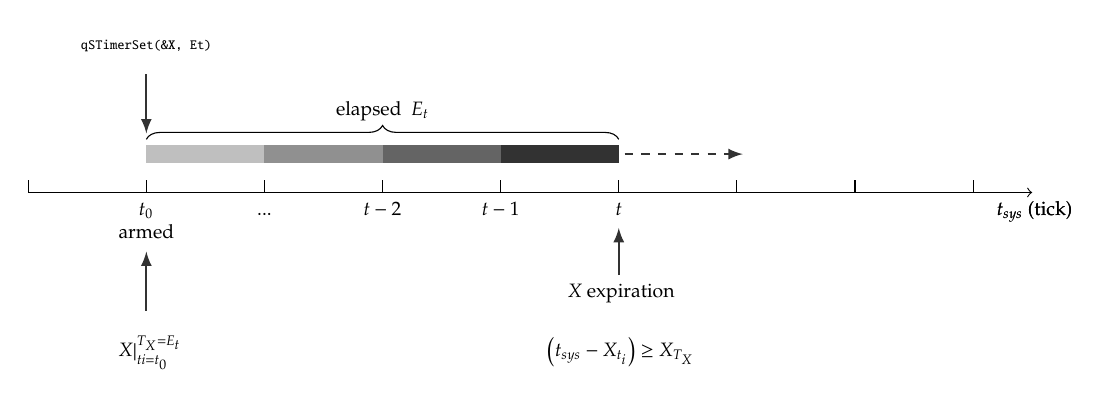
\begin{tikzpicture}[every node/.style= {font=\scriptsize, text height=1ex, text depth=.25ex,},scale=1.5]
        \draw[->] (0,0) -- (8.5,0);
        \foreach \x in {0,1,...,8}{
            \draw (\x cm,3pt) -- (\x cm,0pt);
        }
        \node[anchor=north] at (1,0) {$t_0$};
        \node[anchor=north] at (1,-0.2) {armed};
        \node[anchor=north] at (2,0) {...};
        \node[anchor=north] at (3,0) {$t-2$};
        \node[anchor=north] at (4,0) {$t-1$};
        \node[anchor=north] at (5,0) {$t$};
        \node[anchor=north] at (6,0) {};
        \node[anchor=north] at (8.5,0) {$\ t_{sys}$ (tick)};
        \fill[myLightGray] (1,0.25) rectangle (2,0.4);
        \fill[myDarkGray] (2,0.25) rectangle (3,0.4);
        \fill[myMoreDarkRed] (3,0.25) rectangle (4,0.4);
        \fill[myDeepGray] (4,0.25) rectangle (5,0.4);
        \draw[myDeepGray,dashed,thick,-latex] (5.05,0.325) -- (6.05,0.325);
        \draw[decorate,decoration={brace,amplitude=5pt}] (1,0.45) -- (5,0.45) node[anchor=south,midway,above=4pt] {elapsed $\ E_t$};
        \draw[myDeepGray,thick,-latex] (1,1) -- (1, 0.5 ) node[anchor=north,midway,below=1pt] {};
        \draw[myDeepGray,thick,-latex] (5,-0.7) -- (5, -0.3 ) node[anchor=north,midway,below=1pt] {};
        \draw[myDeepGray,thick,-latex] (1,-1) -- (1, -0.5 ) node[anchor=north,midway,below=1pt] {};
        \node[anchor=north, font=\ttfamily] at (1,1.4) {\tiny qSTimerSet(\&X, Et)};
        \node[anchor=north] at (8.5,0) {$\ t_{sys}$ (tick)};
        \node[anchor=north] at (1,-1.2) {$\ \left.X\right\vert_{ti=t_0}^{T_X=E_t}$};
        \node[anchor=north] at (5,-0.7) {$\ X$ expiration};
        \node[anchor=north] at (5,-1.2) {$\ \left ( t_{sys} - X_{t_i} \right ) \geq X_{T_X}$};
    \end{tikzpicture}
    \caption{STimers operation}
    \label{fig:stimers}
\end{figure}

As illustrated in figure \ref{fig:stimers}, the time expiration check is roll-over safe by restricting it, to the only calculation that make sense for timestamps, $\ t_{sys} - X_{T_x}$, that yields a duration namely the amount of time elapsed between the current instant($\ t_{sys}$ ) and the later instant, specifically, the tick taken at the arming instant with \lstinline{(qSTimer_Set())}, ($\ X_{t_i}$ ).
Thanks to modular arithmetic, both of these are guaranteed to work fine across the clock-source rollover(a 32bit unsigned-counter), at least, as long the delays involved are shorter than 49.7 days. \\

\textbf{Features:}
\begin{itemize}
    \item Provides a non-blocking equivalent to delay function.
    \item Each STimer encapsulates its own expiration (timeout) time.
    \item Provides elapsed and remaining time APIs.
    \item As mentioned before, STimers uses the same kernel clock source, this means the time-elapsed calculation use the \lstinline{qClock_GetTick()} API, therefore, the time resolution has the same value passed when the scheduler has been initialized with \lstinline{qOS_Setup()}.
\end{itemize}

\subsubsection{Using a STimer}
A STimer is referenced by a handle, a variable of type \lstinline{qSTimer_t} \index{\lstinline{qSTimer_t}} and preferably, should be initialized by the \lstinline{QSTIMER_INITIALIZER} constant before any usage. 

To use them, the code should follow a specific pattern that deals with the states of this object. All related APIs are designed to be non-blocking, this means there are ideal for use in cooperative environments as the one provided by the OS itself. To minimize the implementation, this object is intentionally created to behave like a binary object, this implies that it only handles two states, \textit{Armed} and \textit{Disarmed}. 
\newline
An \textit{Armed} timer means that it is already running with a specified preset value and a \textit{Disarmed} timer is the opposite, which means that it doesn't have a preset value, so consequently, it is not running at all.

The arming action can be performed with \lstinline{qSTimer_Set()} \index{\lstinline{qSTimer_Set}} or \lstinline{qSTimer_FreeRun()} \index{\lstinline{qSTimer_FreeRun}} and disarming with \lstinline{qSTimer_Disarm()}.\index{\lstinline{qSTimer_Disarm}} \\

Detailed APIs description is presented below. ( For \lstinline{qSTimer_Disarm()} ignore the \lstinline{Time} argument.)\\

\begin{lstlisting}[style=CStyle]
qBool_t qSTimer_Set( qSTimer_t * const obj, const qTime_t Time )
\end{lstlisting}

\begin{lstlisting}[style=CStyle]
qBool_t qSTimer_FreeRun( qSTimer_t * const obj, const qTime_t Time )
\end{lstlisting}

\begin{lstlisting}[style=CStyle]
void qSTimer_Disarm( qSTimer_t * const obj )
\end{lstlisting}

\subsubsection*{Parameters}
\begin{itemize}
    \item \lstinline{obj} : A pointer to the STimer object. 
    \item \lstinline{Time} : The expiration time(must be specified in seconds).
\end{itemize}

Here, \lstinline{qSTimer_FreeRun()} is a more advanced API, it checks the timer and performs the arming. If disarmed, it gets armed immediately with the specified time. If armed, the time argument is ignored and the API only checks for expiration. When the time expires, the STimer gets armed immediately taking the specified time.

\subsubsection*{Return Value}
For \lstinline{qSTimer_Set()} \lstinline{qTrue} on success, otherwise, returns \lstinline{qFalse}.\\
For \lstinline{qSTimer_FreeRun()} returns \lstinline{qTrue} when the STimer expires, otherwise, returns \lstinline{qFalse}. For a disarmed STimer, also returns \lstinline{qFalse}. \\
None for \lstinline{qSTimer_Disarm()}.

\noindent\hrulefill
\newline
All possible checking actions are also provided for this object, including \lstinline{qSTimer_Elapsed()} \index{\lstinline{qSTimer_Elapsed}}, \lstinline{qSTimer_Remaining()} \index{\lstinline{qSTimer_Remaining}} and \lstinline{qSTimer_Expired()} \index{\lstinline{qSTimer_Expired}}, with the last one being the most commonly used for timing applications.
Finally, to get the current status of the STimer (check if is Armed or Disarmed) the \lstinline{qSTimer_Status()} \index{\lstinline{qSTimer_Status}} API should be used. \\

\begin{lstlisting}[style=CStyle]
qClock_t qSTimer_Elapsed( const qSTimer_t * const obj )
\end{lstlisting}

\begin{lstlisting}[style=CStyle]
qClock_t qSTimer_Remaining( const qSTimer_t * const obj )
\end{lstlisting}

\begin{lstlisting}[style=CStyle]
qBool_t qSTimer_Expired( const qSTimer_t * const obj )
\end{lstlisting}

\begin{lstlisting}[style=CStyle]
qBool_t qSTimer_Status( const qSTimer_t * const obj )
\end{lstlisting}

For this APIs, their only argument, is a pointer to the STimer object.

\subsubsection*{Return Value}
For \lstinline{qSTimer_Elapsed()}, \lstinline{qSTimer_Remaining()} returns the elapsed and remaining time specified in epochs respectively. \\
For \lstinline{qSTimer_Expired()}, returns \lstinline{qTrue} when STimer expires, otherwise, returns \lstinline{qFalse}. For a disarmed STimer, also returns \lstinline{qFalse}. \\
For \lstinline{qSTimer_Status()}, returns \lstinline{qTrue} when armed, and \lstinline{qFalse} for disarmed.

\noindent\hrulefill

\subsubsection*{Usage example:}
The example below shows a simple usage of this object. It is noteworthy that arming is performed once using the \lstinline{FirstCall} flag. This prevents the timer from being re-armed every time the task runs. After the timer expires, it should be disarmed explicitly. \\


\begin{lstlisting}[style=CStyle]
void Example_Task( qEvent_t e ){
    static qSTimer_t timeout = QSTIMER_INITIALIZER;
    if( e->FirstCall ){
        /*Arming the stimer for  3.5 seg*/
        qSTimer_Set( &timeout, 3.5 );
    }
    
    /*non-blocking delay, true when timeout expires*/
    if( qSTimer_Expired( &timeout ) ){
        /*
        TODO: Code when STimer expires
        */    
        qSTimer_Disarm( &timeout );
    }
    else return; /*Yield*/
}
\end{lstlisting}  

\subsection{Finite State Machines (FSM)}
The state machine is one of the fundamental programming patterns. Designers use this approach frequently for solving complex engineering problems. State machines break down the design into a series of finite steps called "states". Each state performs some narrowly defined actions. Events, on the other hand, are the stimuli that cause the state to move or produce a transition between states. 
The provided implementation features a powerful state-machine coding-abstraction including hierarchical patterns and transition tables, allowing the designer to build scalable solutions from simple state-machines to complex statecharts. 

In QuarkTS, states must be defined as functions taking a \lstinline{qSM_Handler_t} object and returning a \lstinline{qSM_Status_t} value. An example is shown in the following code snippet:
\newline

\begin{lstlisting}[style=CStyle]
qSM_Status_t Example_State( qSM_Handler_t m ){
    /*
    TODO: State code
    */
    return qSM_EXIT_SUCCESS;
}
\end{lstlisting}    

Here, the return value represents the finish status of the state, allowing only the values listed below.

\begin{itemize}
    \item \lstinline{qSM_EXIT_SUCCESS(-32768)}.
    \item \lstinline{qSM_EXIT_FAILURE(-32767)}.
    \item Any other integer value between \lstinline{-32766} and \lstinline{32767}.
\end{itemize} 

Every state machine has the concept of \textit{current state} ($P$). This is the state that FSM currently occupies. At any given moment in time, the state machine can be in only a single state. The exit status can be handled with additional \textit{sub-states}($S_{(b,s,u,f)}$) established at the moment of the FSM initialization. This workflow between the \textit{current state} and the \textit{sub-states} is better shown in the graph below: 

\begin{figure}[H]
    \centering
    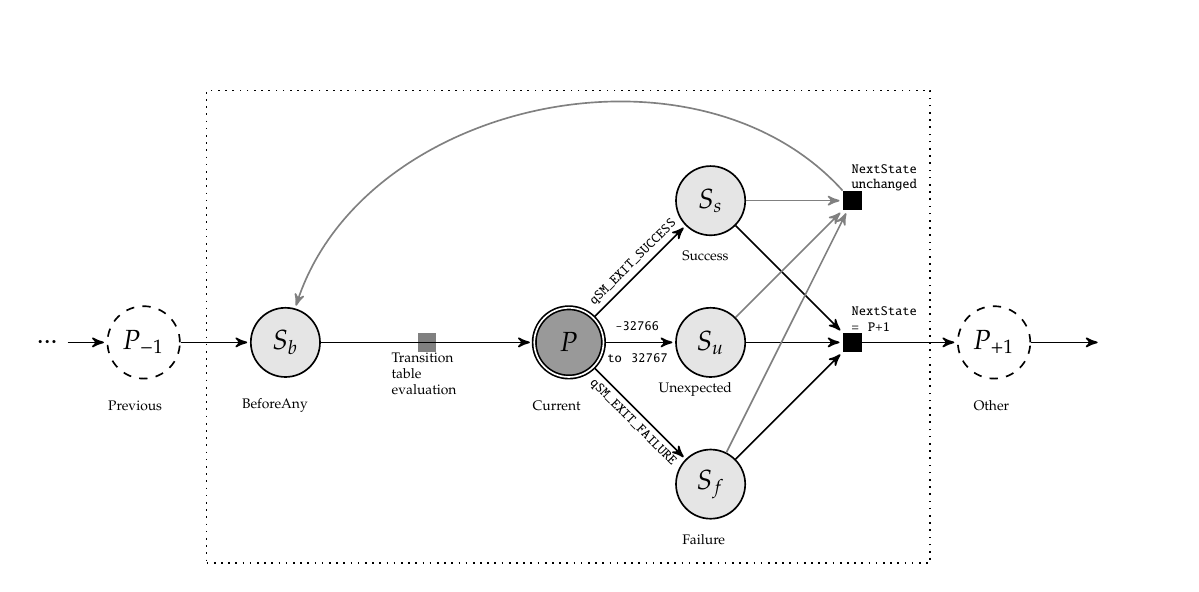
\begin{tikzpicture}[initial text={...}, ->,>=stealth',shorten >=1pt,auto,node distance=1.8cm, semithick]
        \draw[dotted] (0.8,-2.8) -- (9.99,-2.8) -- (9.99,3.2) -- (0.8,3.2) -- (0.8,-2.8 ) -- cycle;
        \node[dashed, initial,state]                    (A)              {$P_{-1}$};
        \node[fill=gray!20, state]                      (B) [right of=A] {$S_b$};
        \node[rectangle, fill=gray]                    (W) [right of=B] {};
        \node[fill=gray!80, state, accepting]           (C) [right of=W] {$P$};
        \node[fill=gray!20, state]                      (D) [right of=C] {$S_u$};
        \node[fill=gray!20, state]                      (E) [above of=D] {$S_s$};
        \node[fill=gray!20, state]                      (F) [below of=D] {$S_f$};
        \node[rectangle, fill=black]                    (T) [right of=D] {};
        \node[dashed, state]                            (G) [right of=T] {$P_{+1}$};
        \node[rectangle, fill=black]                    (R) [above of=T] {};
        \node[state,draw=none]                          (H) [right of=G] {};
        \node at (9.99, 0.4)   (D1) [font=\ttfamily, text width=2cm]{\tiny NextState};    
        \node at (9.99, 0.2)   (D2) [font=\ttfamily, text width=2cm]{\tiny = P+1};  
        \node at (9.99, 2.2)   (D3) [font=\ttfamily, text width=2cm]{\tiny NextState};
        \node at (9.99, 2.0)   (D4) [font=\ttfamily, text width=2cm]{\tiny unchanged};
        \node at (6.40, 1.2)   (D4) [font=\ttfamily, text width=2cm, rotate=45]{\tiny qSM\_EXIT\_SUCCESS};
        \node at (6.4, -1.2)   (D4) [font=\ttfamily, text width=2cm, rotate=-45]{\tiny qSM\_EXIT\_FAILURE};
        \node at (6.99, 0.2)   (D4) [font=\ttfamily, text width=2cm]{\tiny -32766};
        \node at (6.89, -0.2)   (D4) [font=\ttfamily, text width=2cm]{\tiny to 32767};
        \node at (0.3,-0.8)   (D5) [text width=1.5cm]{\tiny Previous};    
        \node at (2.0,-0.8)   (D6) [text width=1.5cm]{\tiny BeforeAny};
        \node at (3.9,-0.2)   (DX) [text width=1.5cm]{\tiny Transition};
        \node at (3.9,-0.4)   (DY) [text width=1.5cm]{\tiny table};
        \node at (3.9,-0.6)   (DY) [text width=1.5cm]{\tiny evaluation};
        \node at (5.69,-0.8)   (D7) [text width=1.5cm]{\tiny Current};
        \node at (7.59,1.1)    (D8) [text width=1.5cm]{\tiny Success};
        \node at (7.29,-0.6)   (D9) [text width=1.5cm]{\tiny Unexpected};
        \node at (7.59,-2.5)   (DA) [text width=1.5cm]{\tiny Failure};
        \node at (11.29,-0.8)   (DB) [text width=1.5cm]{\tiny Other};

        \path   (A) edge node {} (B)
                (B) edge node {} (C) 
                (C) edge []  node {} (D)
                (C) edge []  node {} (E)
                (C) edge []  node {} (F)
                (D) edge []  node {} (T)
                (E) edge []  node {} (T)
                (F) edge []  node {} (T)
                (D) edge [gray] node {} (R)
                (E) edge [gray] node {} (R)
                (F) edge [gray] node {} (R)
                (R) edge [gray, bend left=-60] node {} (B)
                (T) edge node {} (G)
                (G) edge node {} (H);
    \end{tikzpicture}
    \caption{Sub-states evaluated after and before the \textit{current} state}
    \label{fig:substates}
\end{figure}

Figure \ref{fig:substates} shows that these \textit{sub-states} (if enabled) are implicitly linked in the workflow to every state in the FSM. These \textit{sub-states}, and the way they are called are described below:

\begin{itemize}
    \item \textit{BeforeAny} ($S_b$) : Performed in every FSM cycle. As its name implies, it is launched before the \textit{current state} executes. 
    
    \item \textit{Success} ($S_s$) : This \textit{sub-state} is conditioned to the exit status of the \textit{current state}. If \textit{current state} has exited with  \lstinline{qSM_EXIT_SUCCESS}, this sub-state will be launched next. It can be used to perform the actions of the \textit{current state}, for example, if a certain state is controlling an output, its value would only be written if the state has ended correctly.
    
    \item \textit{Failure} ($S_f$): Same behavior as the previous one, but instead, is conditioned to the exit value \lstinline{qSM_EXIT_FAILURE}. It can be used to handle exceptions.
    
    \item \textit{Unexpected} ($S_u$): Same behavior as \textit{Failure} and \textit{Success}, but instead, is conditioned to an exit value between \lstinline{-32766} and \lstinline{32767}. The applications for this sub-state should be defined by the application writer.
\end{itemize}


\subsubsection{Setting up a state machine : \lstinline{qStateMachine_Setup} }
Like any other OS object, a Finite State Machine (FSM) must be explicitly initialized before it can be used. FSMs are referenced by handles, which are variables of type \lstinline{qSM_t}. \index{\lstinline{qSM_t}}

The \lstinline{qStateMachine_Setup()} API \index{\lstinline{qStateMachine_Setup}}  initializes the instance, sets the initial state and conditioned sub-states.\\


\begin{lstlisting}[style=CStyle]
qBool_t qStateMachine_Setup( qSM_t * const obj, qSM_State_t InitState,
                             qSM_SubState_t SuccessState, 
                             qSM_SubState_t FailureState, 
                             qSM_SubState_t UnexpectedState, 
                             qSM_SubState_t BeforeAnyState )
\end{lstlisting}

\subsubsection*{Parameters}
\begin{itemize}
    \item \lstinline{obj} : A pointer to the FSM object.
    \item \lstinline{InitState} :  The first state to be performed. This argument is a pointer to a callback function, returning \lstinline{qSM_Status_t} and with a \lstinline{qSM_Handler_t} variable as input argument.
    \item \lstinline{SuccessState} :  Sub-State performed after a state exits with  \lstinline{qSM_EXIT_SUCCESS}. 
    \item \lstinline{FailureState} :  Sub-State performed after a state exits with  \lstinline{qSM_EXIT_FAILURE}. 
    \item \lstinline{UnexpectedState} :  Sub-State performed after a state exits with any value between \lstinline{-32766} and \lstinline{32767}. 
    \item \lstinline{BeforeAnyState} :  A state called before the normal state machine execution.
\end{itemize}  

\begin{tcolorbox}
\ArrowBoldDownRight \textit{Note}: For every sub-state argument, a \lstinline{NULL} value will act as a "disable" action.
\end{tcolorbox}

Unlike normal states, a sub-state should not return anything, thus, the callback for substates should be written as: \\

\begin{lstlisting}[style=CStyle]
void SubState_Example( qSM_Handler_t m ){
    /*
    TODO: Sub-State code
    */
}
\end{lstlisting}  

\subsubsection{Running a state machine : \lstinline{qStateMachine_Run} }
This API \index{\lstinline{qStateMachine_Run}} is used to execute the Finite State Machine. Only a single cycle is performed invoking the callback of the current active state (including nested states of the hierarchical topology), and of course, the available sub-states according to figure \ref{fig:substates}. \\

\begin{lstlisting}[style=CStyle]
void qStateMachine_Run( qSM_t * const obj, void *Data )
\end{lstlisting}

\subsubsection*{Parameters}
\begin{itemize}
    \item \lstinline{obj} : a pointer to the FSM object.
    \item \lstinline{Data} : FSM associated data. Also can be used to represent the FSM arguments. All arguments must be passed by reference and cast to (\lstinline{void *}). For multiple data, create a structure and pass a pointer to that structure.  
\end{itemize}  

\subsubsection{Changing states and retrieving FSM data}
Both, states and sub-states callbacks take a \lstinline{qSM_Handler_t} \index{\lstinline{qSM_Handler_t}} object as input argument, which is basically a pointer to the involved properties of the invoking FSM. The usage of this object it's required to make the FSM moves between states and additionally get extra execution data. The provided fields are:

\begin{itemize}
    \item \lstinline{NextState} : The next state to be executed after the current state finishes. The application writer should change this field to another state callback to produce a state transition in the next FSM's cycle.
    \item \lstinline{PreviousState} (read-only):  Last state seen in the flow chart.
    \item \lstinline{LastState} (read-only):  The last state executed.
    \item \lstinline{PreviousReturnStatus} (read-only): The exit(or return) status of the previous state.
    \item \lstinline{LastReturnStatus} (read-only): The exit(or return) status of the last state.
    \item \lstinline{Signal} (read-only): Received signal. \lstinline{QSM_SIGNAL_NONE} if no signal available. \lstinline{QSM_SIGNAL_ENTRY} if the current state has just entered from another state. \lstinline{QSM_SIGNAL_EXIT} if the current state has just exit to another state. Any other user-defined signal will reside here if the FSM has a signal-queue installed .
    \item \lstinline{Data} (read-only): State-machine associated data. If the FSM is running as a task, the associated event data can be queried through this field. (here, a cast to \lstinline{qEvent_t} is mandatory). Child FSMs inherit this member.
    \item \lstinline{Parent} (read-only): A pointer to the parent state-machine. Can be used in hierarchical  patterns. \lstinline{NULL} if the FSM its not a child.
\end{itemize}

The developer is free to write and control state transitions. A state jumps from one to another by changing the \lstinline{NextState} field. Any transition is allowed at any time.

The code snippet below shows how this input argument should be used to produce a state transition and obtain additional information: \\

\begin{lstlisting}[style=CStyle]
qSM_Status_t Some_State( qSM_Handler_t m ){
    qSM_Status_t RetValue = qSM_EXIT_SUCCESS;
    
    switch( m->Signal ){
        case QSM_SIGNAL_ENTRY:
            /*
                TODO : Do something at the first entry
            */        
            break;
        case QSM_SIGNAL_EXIT:
            break;
        default:
            /*
                TODO : Whatever this state does
            */
            if ( EVENT_A_RECEIVED() ){ /*this it a state transition*/
                m->NextState = Other_State; 
                /*it will be executed in the next cycle*/
            }
            
            if ( EVENT_B_RECEIVED() ){ /*this it a state transition*/
                m->NextState = m->PreviousState; 
                /*return to the previous state*/ 
                /*it will be executed in the next cycle*/
                /*this transition has the higher priority*/
            }       
            
            if ( EVENT_ERROR_RECEIVED() ){ 
                RetValue = qSM_EXIT_FAILURE;
            }
            break;
    }
    return RetValue;
}
\end{lstlisting}  

\subsubsection{Adding a state machine as a task : \lstinline{qOS_Add_StateMachineTask} } \label{statemachinetask}
The best strategy to implement a FSM is delegating it to a task. For this, the provided \index{\lstinline{qOS_Add_StateMachineTask}} API should be used. Here, the task doesn't have a specific callback, instead, it will evaluate the active state of FSM, and later, all the other possible states in response to events that mark their own transition. The task will be scheduled to run every \lstinline{Time} seconds in \lstinline{qPeriodic} mode. 


Using this API, the kernel will take care of the FSM by itself, so the usage of \lstinline{qStateMachine_Setup()} and \lstinline{qStateMachine_Run()} can be omitted. \\

\begin{lstlisting}[style=CStyle]
qBool_t qOS_Add_StateMachineTask( 
            qTask_t * const Task, qPriority_t Priority, qTime_t Time,
            qSM_t * const StateMachine, qSM_State_t InitState, 
            qSM_SubState_t BeforeAnyState, qSM_SubState_t SuccessState, 
            qSM_SubState_t FailureState, qSM_SubState_t UnexpectedState,
            qState_t InitialTaskState, void *arg )
\end{lstlisting}

\subsubsection*{Parameters}
\begin{itemize}
    \item \lstinline{Task} : A pointer to the task node. 
    \item \lstinline{Priority} : The priority value. [0(min) - \lstinline{Q_PRIORITY_LEVELS}(max)]
    \item \lstinline{Time} : Execution interval defined in seconds (floating-point format). For immediate execution use the  \lstinline{qTimeImmediate} definition. 
    \item \lstinline{StateMachine} : A pointer to Finite State-Machine (FSM) object.
    \item \lstinline{InitState} :  The first state to be performed. 
    \item \lstinline{BeforeAnyState} :  The sub-state called before any current state.
    \item \lstinline{SuccessState} :  Sub-State performed after a state exits with \lstinline{qSM_EXIT_SUCCESS}.
    \item \lstinline{FailureState} :  Sub-State performed after a state exits with \lstinline{qSM_EXIT_FAILURE}.
    \item \lstinline{UnexpectedState } : Sub-State performed after a state exits with any value between \lstinline{-32766} and \lstinline{32767}.      
    \item \lstinline{TaskInitState } : Specifies the initial operational state of the task (\lstinline{qEnabled}, \lstinline{qDisabled}, \lstinline{qAsleep} or \lstinline{qAwake}).
    \item \lstinline{arg} - Represents the task arguments. All arguments must be passed by reference and cast to \lstinline{(void *)}. 
\end{itemize}

\begin{tcolorbox}
\ArrowBoldDownRight \textit{Note}: For every sub-state argument, a \lstinline{NULL} value will act as a disable action.
\end{tcolorbox}

Now that a task is running a dedicated state-machine, the specific task event-info can be obtained in every state callback through the \lstinline{Data} field of the \lstinline{qSM_Handler_t} argument. Check the example below: \\

\begin{lstlisting}[style=CStyle]
qSM_Status_t Example_State( qSM_Handler_t m ){
    qEvent_t e = m->Data; 
    /* Get the event info of the task that owns this state-machine*/
    switch( m->Signal ){
        case QSM_SIGNAL_ENTRY:
            break;
        case QSM_SIGNAL_EXIT:
            break;
        default:
            switch( e->Trigger ){
                case byTimeElapsed:
                    /* TODO: Code for this case */
                break;
                case byNotificationSimple:
                    /* TODO: Code for this case */
                break;
                case byQueueCount:
                    /* TODO: Code for this case */
                break;
                default: break;
            }
            /* TODO: State code */
            break;
    }
    return qSM_EXIT_SUCCESS;
}
\end{lstlisting}

\subsubsection{A demonstrative example} \label{fsm_example}
In this example, one press of the button turn on the LED, a second push of the button will make the LED blink and if the button is pressed again, the LED will turn off. Also, our system must turn off the LED after a period of inactivity. If the button hasn't been pressed in the last 10 seconds, the LED will turn off. 

States ($\ S_i$) and transitions ($\ t_i$) are described as follows: \\
\begin{itemize}
\begin{minipage}{0.4\linewidth}
    \item $\ S_1$ : LED Off
    \item $\ S_2$ : LED On
    \item $\ S_3$ : LED Blink
\end{minipage}
\begin{minipage}{0.4\linewidth}
    \item $\ t_1$ : Button press (rising edge)
    \item $\ t_2$ : Timeout (10S)
\end{minipage}
\end{itemize}

\begin{figure}[H]
    \centering 
    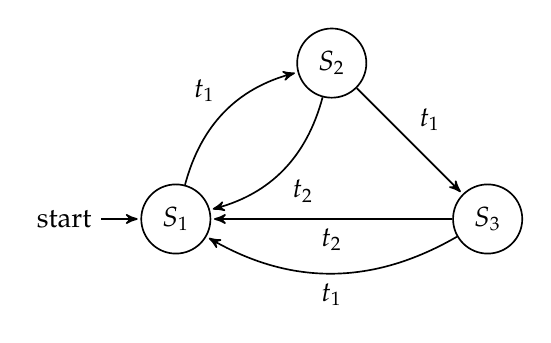
\begin{tikzpicture}[->,>=stealth',shorten >=1pt,auto,node distance=2.8cm, semithick]
        \node[initial,state] (A)                    {$S_1$};
        \node[state]         (B) [above right of=A] {$S_2$};
        \node[state]         (C) [below right of=B] {$S_3$};
    
        \path   (A) edge [bend left]  node {$t_1$} (B)
                (B) edge              node {$t_1$} (C)
                (C) edge [bend left]  node {$t_1$} (A)
                (C) edge              node {$t_2$} (A)
                (B) edge [bend left]  node {$t_2$} (A);
    \end{tikzpicture}
    \caption{A simple FSM example with three states}
    \label{fig:fsmexample}
\end{figure}

To start the implementation, let's define the necessary global variables...

\begin{lstlisting}[style=CStyle]
qTask_t LED_Task; /*The task node*/
qSM_t LED_FSM; /*The state-machine handle*/
\end{lstlisting}

Then, we define our states as the flow-diagram showed in figure \ref{fig:fsmexample}.

\begin{lstlisting}[style=CStyle]
qSM_Status_t State_LED_Off( qSM_Handler_t m ){
    switch( m->Signal ){
        case QSM_SIGNAL_ENTRY:
            BSP_LED_OFF();
            break;
        default:
            if( BUTTON_PRESSED ){
                m->NextState = State_LED_On;
            }
            break;
    }
    return qSM_EXIT_SUCCESS;
}
/*---------------------------------------------------------------------*/
qSM_Status_t State_LED_On( qSM_Handler_t m ){
    static qSTimer_t timeout;
    switch( m->Signal ){
        case QSM_SIGNAL_ENTRY:
            qSTimer_Set( &timeout, 10.0 ); /*STimer gets armed*/
            BSP_LED_ON();
            break;
        default:
            if( qSTimer_Expired( &timeout) ){ /*check if the timeout expired*/
                m->NextState = State_LED_Off;
            }
            if( BUTTON_PRESSED ){
                m->NextState = State_LED_Blink;
            }
            break;
    }
    return qSM_EXIT_SUCCESS;
}
/*---------------------------------------------------------------------*/
qSM_Status_t State_LED_Blink( qSM_Handler_t m ){
    static qSTimer_t timeout;
    static qSTimer_t blinktime;
    
    switch( m->Signal ){
        case QSM_SIGNAL_ENTRY:
            qSTimer_Set( &timeout, 10.0 );
            break;
        default:
            if( qSTimer_Expired( &timeout ) || BUTTON_PRESSED ){
                m->NextState = State_LED_Off;
            }
            if( qSTimer_FreeRun( &blinktime, 0.5 ) ){
               BSP_LED_TOGGLE();
            }
            break;
    }
    return qSM_EXIT_SUCCESS;
}
\end{lstlisting}

Finally, we add the task to the scheduling scheme running the dedicated state machine. \\

Remember that you must set up the scheduler before adding a task to the scheduling scheme. \\

\begin{lstlisting}[style=CStyle]
qOS_Add_StateMachineTask( &LED_Task, qHigh_Priority, 0.1, &LED_FSM,
                          State_LED_Off, NULL, NULL, NULL, NULL,
                          qEnabled, NULL);
\end{lstlisting}

\subsubsection{Changing the FSM attributes in run-time}
For this, use the API \index{\lstinline{qStateMachine_Attribute}} that is detailed below:\\

\begin{lstlisting}[style=CStyle]
void qStateMachine_Attribute( 
                        qSM_t * const obj, const qSM_Attribute_t Flag, 
                        qSM_State_t  s, qSM_SubState_t subs )
\end{lstlisting}

\begin{itemize}
    \item \lstinline{obj} : A pointer to the FSM object.
    \item \lstinline{Flag} : The attribute/action to be taken. Should be one of the following:
    \begin{itemize}
        \item \lstinline{qSM_RESTART} : Restart the FSM (here, the \lstinline{s} argument must correspond to the init-state)
        \item \lstinline{qSM_CLEAR_STATE_FIRST_ENTRY_FLAG} : clear the entry flag for the current state if the \lstinline{NextState} field doesn't change.
        \item \lstinline{qSM_FAILURE_STATE} : Set the failure sub-state.
        \item \lstinline{qSM_SUCCESS_STATE} : Set the success sub-state.
        \item \lstinline{qSM_UNEXPECTED_STATE} : Set the unexpected sub-state.
        \item \lstinline{qSM_BEFORE_ANY_STATE} : Set the sub-state executed before any state.
        \item \lstinline{qSM_UNINSTALL_TRANSTABLE} : To uninstall the transition table if available.
    \end{itemize}
    \item \lstinline{s} : The new value for state (only applies in \lstinline{qSM_RESTART}). If not used, pass \lstinline{NULL}.
    \item \lstinline{subs} : The new value for sub-state (only apply in \lstinline{qSM_FAILURE_STATE}, \lstinline{qSM_SUCCESS_STATE}, \lstinline{qSM_UNEXPECTED_STATE} and \lstinline{qSM_BEFORE_ANY_STATE}. If not used, pass \lstinline{NULL}.
\end{itemize}

\subsubsection{Using a transition table}
In this approach, the FSM is coded in a table relating states and signal-events. 
This is an elegant method to translate the FSM to actual implementation as the handling for every state and event combination is encapsulated in the table. 

\begin{table}[h!]
\centering
\begin{tabular}{||c c c c c c||} 
 \hline
 \textit{Current} & \textit{Signal} & \textit{Next} & \textit{Signal action} & \textit{Target FSM} & \textit{Next in target} \\ [0.5ex] 
 
 \hline\hline
 \ttfamily{StateA} & \ttfamily{Signal1} & \ttfamily{StateB} & \ttfamily{NULL} & \ttfamily{NULL} & \ttfamily{NULL} \\ 
 \ttfamily{StateB} & \ttfamily{Signal3} & \ttfamily{StateD} & \ttfamily{DoOnSignal3}& \ttfamily{NULL} & \ttfamily{NULL}   \\
 ... & ... & ... & ... & ... &...\\
 \ttfamily{StateD} & \ttfamily{Signal6} & \ttfamily{StateA} & \ttfamily{NULL} & \ttfamily{NULL} & \ttfamily{NULL}\\ [1ex] 
 \hline
\end{tabular}
\caption{Transition table layout in QuarkTS}
\label{ttable_layout}
\end{table}

Here, the application writer get a quick picture of the FSM and the embedded software maintenance is also much more under control. A transition table is referenced through an object of type \lstinline{qSM_TransitionTable_t} and should be explicitly installed in the target FSM with the corresponding entries, an \textit{n}-sized array of \lstinline{qSM_Transition_t} elements. 

Events on the other hand, are represented in the table with FSM-Signals, an unsigned number of type \lstinline{qSM_Signal_t}. Here, the designer is free to name event signals according the FSM application. 

The API \lstinline{qStateMachine_TransitionTableInstall()}, should be used to perform the transition table installation to the target FSM. \\

\begin{lstlisting}[style=CStyle]
qBool_t qStateMachine_TransitionTableInstall( qSM_t * const obj,   
            qSM_TransitionTable_t *table, qSM_Transition_t *entries, 
            size_t NoOfEntries )
\end{lstlisting} \index{\lstinline{qStateMachine_TransitionTableInstall}}

\subsubsection*{Parameters}
\begin{itemize}
    \item \lstinline{obj} : A pointer to the FSM object. 
    \item \lstinline{table} : A pointer to the transition table instance.
    \item \lstinline{entries} : The array of transitions (\lstinline{qSM_Transition_t[]}). 
    \item \lstinline{NoOfEntries} : The number of transitions inside \lstinline{entries}.
\end{itemize}

\subsubsection*{Return Value}
Returns \lstinline{qTrue} on success, otherwise returns \lstinline{qFalse}.

\hrulefill

\subsubsection*{Caveats}
\begin{itemize}
    \item State transitions are not limited to the specification of the transition table. A state callback owns the higher precedence to change a state. The application writer can use both, a transition table and direct \lstinline{NextState} field manipulation in state callbacks to perform a transition to the FSM.
    \item Special care is required when the table grows very large, that is, when there are many invalid state/event combinations, leading to a waste of memory. There is also a memory penalty as the number of states and events grow. The application writer  need to accurately account for this during initial design. A statechart pattern can be used to improve the design and reduce the number of transition entries. 
    \item As shown in figure \ref{fig:substates}, an installed transition table is evaluated after the \textit{BeforeAny} sub-state, and later, the current state handler will be evaluated after the table sweep is completed. In summary, the state handler has a higher precedence over the table to perform state transitions.
\end{itemize}

\paragraph{Signals in transition tables:}
When using transition tables, signals are the selected event-abstraction to produce a transition from one state to another. Signals can be asynchronously delivered to the FSM, as they are handled internally with an exclusive FIFO queue. 
The signal queue should be installed with \lstinline{qStateMachine_SignalQueueSetup} after the FSM setup. \\

\begin{lstlisting}[style=CStyle]
qBool_t qStateMachine_SignalQueueSetup( qSM_t * const obj, 
                                        qSM_Signal_t *AxSignals, 
                                        size_t MaxSignals )
\end{lstlisting} \index{\lstinline{qStateMachine_SignalQueueSetup}}

\subsubsection*{Parameters}
\begin{itemize}
    \item \lstinline{obj} : A pointer to the FSM object. 
    \item \lstinline{AxSignals} : A pointer to signal-queue storage area. A n-array of type \lstinline{qSM_Signal_t[]}.
    \item \lstinline{MaxSignals} : The number of event-signals that the queue can hold.
\end{itemize}

\subsubsection*{Return Value}
\lstinline{qTrue} on success, otherwise returns \lstinline{qFalse}.

\hrulefill
\newline

To perform a signal delivering to a FSMs, the following API should be used: \\

\begin{lstlisting}[style=CStyle]
qBool_t qStateMachine_SendSignal( qSM_t * const obj, qSM_Signal_t signal, 
                                  qBool_t isUrgent )
\end{lstlisting} \index{\lstinline{qStateMachine_SendSignal}}

\subsubsection*{Parameters}
\begin{itemize}
    \item \lstinline{obj} : A pointer to the FSM object. 
    \item \lstinline{signal} : The user-defined signal.
    \item \lstinline{isUrgent} : If \lstinline{qTrue}, the signal will be sent to the front of the transition-table queue.
\end{itemize}

\subsubsection*{Return Value}
\lstinline{qTrue} if the provided signal was successfully delivered to the FSM, otherwise return \lstinline{qFalse}.

\hrulefill
\newline

\begin{tcolorbox}
\HandRight A FSM can be better exploited if it has both features, the signal queue and the transition table.
\end{tcolorbox}

\begin{tcolorbox}
\ArrowBoldDownRight \textit{Note}: When a transition entry is defined. the event-signal should be located as the second parameter of the entry. Please see the transition layout in table \ref{ttable_layout}.
\end{tcolorbox}

\paragraph{Signal actions and guards:} Transition tables allow the usage of this feature. When an event-signal is received from the queue, the signal-action, if available, is evaluated before the transition is triggered. This action is user-defined and should be coded as a function that takes a \lstinline{qSM_Handler_t} object and returns a value of type \lstinline{qBool_t}. \\

\begin{lstlisting}[style=CStyle]
qBool_t Signal_Action( qSM_Handler_t ){
    /* TODO : Event-signal action*/
    return qTrue; /*allow the state transition*/
}
\end{lstlisting}

\newline

The return value is checked after to allow or reject the state transition. The application writer can code a boolean expression to implement statechart guards or perform some pre-transition procedure.

\begin{tcolorbox}
\HandRight If a signal-action returns \lstinline{qFalse}, the event-signal is rejected, preventing the state transition to be performed in the calling FSM.
\end{tcolorbox}

\begin{tcolorbox}
\ArrowBoldDownRight \textit{Note}: When a transition entry is defined. the signal-action should be located as the fourth parameter of the entry. Please see the transition layout in table \ref{ttable_layout}.
A \lstinline{NULL} value will act as a NOT-defined, always allowing the state-transition. 
\end{tcolorbox}

\paragraph{Signal responsiveness in state-machine tasks :}

When using state-machine tasks, there is no relationship between transition-table signals and task events by default, this means that tasks cannot be changed to \textit{qReady} immediately if a signal is received, as consequence, the FSM can lose responsiveness to incoming signals because they are only served when the task is triggered by another kind of events. 

To overcome this special situation, the following OS API should be invoked: \\

\begin{lstlisting}[style=CStyle]
qBool_t qOS_StateMachineTask_SigCon( qTask_t * const Task )
\end{lstlisting} \index{\lstinline{qOS_StateMachineTask_SigCon}}

This API performs a kernel connection between the FSM signal-queue and the FSM-task, allowing the OS to catch signals to produce a task event, resulting in a faster handling of incoming signals. \\

\begin{tcolorbox}
\HandRight This API should only be invoked after the FSM-task is added to the scheme.
\end{tcolorbox}

\begin{tcolorbox}
\HandRight This API doesn't have any effect if the FSM is not attached to a task.
\end{tcolorbox}

\paragraph{Demonstrative example using a transition table}
The following example shows the implementation of the FSM presented in section \ref{fsm_example} using a transition table approach.

Before getting started, the required variables should be defined: \\

\begin{lstlisting}[style=CStyle]
/*define the FSM application event-signals*/
#define SIGNAL_BUTTON_PRESSED  ( (qSM_Signal_t)1 )
#define SIGNAL_TIMEOUT         ( (qSM_Signal_t)2 )

qTask_t LED_Task; /*The task node*/
qSM_t LED_FSM; /*The state-machine handler*/
qSM_TransitionTable_t LED_FSM_TransTable; /*the FSM transition table*/

/*create the transition table entries with the desired FSM behavior*/
qSM_Transition_t LED_FSM_TransEntries[] = {
{ State_LED_Off, SIGNAL_BUTTON_PRESSED, State_LED_On, NULL, NULL, NULL },
{ State_LED_On, SIGNAL_TIMEOUT, State_LED_Off, NULL, NULL, NULL },
{ State_LED_On, SIGNAL_BUTTON_PRESSED, State_LED_Blink, NULL, NULL, NULL },
{ State_LED_Blink, SIGNAL_TIMEOUT, State_LED_Off, NULL, NULL, NULL },
{ State_LED_Blink, SIGNAL_BUTTON_PRESSED, State_LED_Off, NULL, NULL, NULL }
};

/*create the memory area for the signal-queue*/
qSM_Signal_t LED_FSM_SignalArea[4];
/*the timeout object*/
qSTimer_t LED_FSM_Timeout = QSTIMER_INITIALIZER;
\end{lstlisting}

Then, we define the callback for the states. Here, the \lstinline{BeforeAny} sub-state is defined to send the timeout signal. \\

\begin{lstlisting}[style=CStyle]
void SubState_LED_BeforeAny( qSM_Handler_t m ){
    if( qSTimer_Expired( &LED_FSM_Timeout ) ){
        qStateMachine_SendSignal( &LED_FSM, SIGNAL_TIMEOUT, qFalse );
    }
}
/*---------------------------------------------------------------------*/
qSM_Status_t State_LED_Off( qSM_Handler_t m ){
    switch( m->Signal ){
        case QSM_SIGNAL_ENTRY:
            BSP_LED_OFF();
            break;
        default:
            break;
    }
    return qSM_EXIT_SUCCESS;
}
/*---------------------------------------------------------------------*/
qSM_Status_t State_LED_On( qSM_Handler_t m ){
    switch( m->Signal ){
        case QSM_SIGNAL_ENTRY:
            qSTimer_Set( &LED_FSM_Timeout, 10.0 ); /*STimer gets armed*/
            BSP_LED_ON();
            break;
        default:
            break;    
    }
    return qSM_EXIT_SUCCESS;
}
/*---------------------------------------------------------------------*/
qSM_Status_t State_LED_Blink( qSM_Handler_t m ){
    static qSTimer_t blinktime;
    switch( m->Signal ){
        case QSM_SIGNAL_ENTRY:
            qSTimer_Set( &LED_FSM_Timeout, 10.0 );
            break;
        default:
            if( qSTimer_FreeRun( &blinktime, 0.5 ) ){
                BSP_LED_TOGGLE();
            }        
            break;        
    }
    return qSM_EXIT_SUCCESS;
}
\end{lstlisting}

In the previous code snippet, we assumed that \lstinline{SIGNAL_BUTTON_PRESSED} can be delivered from either the interrupt context or another task.

To finish the setup, a task is added to handle the FSM and then, the transition table can be installed. \\

\begin{lstlisting}[style=CStyle]
qOS_Add_StateMachineTask( &LED_Task, qHigh_Priority, 0.1, &LED_FSM, 
                          State_LED_Off, SubState_LED_BeforeAny, 
                          NULL, NULL, NULL, qEnabled, NULL );
                          
qStateMachine_TransitionTableInstall( &LED_FSM, &LED_FSM_TransTable,   
                                     LED_FSM_TransEntries, 5 );
                                     
qStateMachine_SignalQueueSetup( &LED_FSM, LED_FSM_SignalArea, 4 ):

/*improve the transition table signal-response*/                                    
qOS_StateMachineTask_SigCon( &LED_Task );  
\end{lstlisting}

\paragraph{Composite states, the hierarchical approach : } A composite state is defined as state that has inner states (a nested state-machine running inside the state). A composite state is a decomposition mechanism that allows factoring of common behaviors and their reuse. This allow to model the state-machine using a hierarchical pattern (aka statecharts). 

In conventional state machine designs, all states are considered at the same level. The design does not capture the commonality that exists among states. In real life, many states handle most transitions in similar fashion and differ only in a few key components. Even when the actual handling differs, there is still some commonality.

Hierarchical state machine design captures the commonality by organizing the states as a hierarchy. The states at the higher level in hierarchy perform the common handling, while the lower level states inherit the commonality from higher level ones and perform the state specific functions. 

To setup a composite state, the following API should be used: \\

\begin{lstlisting}[style=CStyle]
qBool_t qStateMachine_Set_CompositeState( qSM_t * const parent, 
                                          qSM_State_t state, 
                                          qSM_t * const child )
\end{lstlisting}

\begin{itemize}
    \item \lstinline{parent} : A pointer to the parent FSM object.
    \item \lstinline{state} : A state from \lstinline{parent} to relate the \lstinline{child} FSM. This state will be set as composite.
    \item \lstinline{child} : A pointer to the child FSM object who becomes part of the composite state.
\end{itemize}

\subsubsection*{Return Value}
Returns \lstinline{qTrue} on success, otherwise returns \lstinline{qFalse};

\hrulefill
\newline

\begin{tcolorbox}
\HandRight If the child FSM doesn't have a signal-queue defined, the parent signal will be propagated to it.
\end{tcolorbox}


\paragraph{Demonstrative example using a composite state :} This example takes the "Cruise Control" study case from \cite{gomaa}, a real-time system that manages the speed of an automobile based on inputs from the driver. 

The behavior of this system is state-dependent in that the executed actions correspond not only to the driver input, but also on the current state of the system and with the status of the engine and the brake. 
The figure \ref{fig:fsmej} illustrate the modeling of this system with the "Automated Control" state acting as composite. \\



\begin{tcolorbox}
\HandRight Transitions to a specific state inside a composite state and vice versa, should be parametrized in the last two parameters of the transition entry. Please see the transition layout in table \ref{ttable_layout}.
\end{tcolorbox}

\begin{figure}[H]
    \centering



\tikzset{every picture/.style={line width=0.75pt}} %set default line width to 0.75pt        

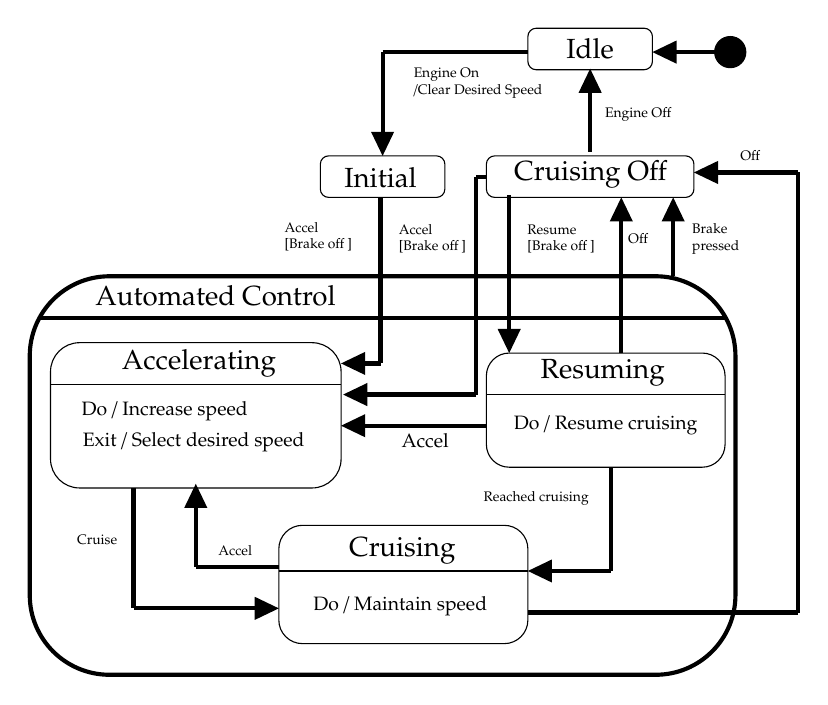
\begin{tikzpicture}[x=0.75pt,y=0.75pt,yscale=-1,xscale=1]
%uncomment if require: \path (0,423); %set diagram left start at 0, and has height of 423

%Rounded Rect [id:dp6662432613291265] 
\draw   (350,77.5) .. controls (350,75.29) and (351.79,73.5) .. (354,73.5) -- (406,73.5) .. controls (408.21,73.5) and (410,75.29) .. (410,77.5) -- (410,89.5) .. controls (410,91.71) and (408.21,93.5) .. (406,93.5) -- (354,93.5) .. controls (351.79,93.5) and (350,91.71) .. (350,89.5) -- cycle ;
%Rounded Rect [id:dp6675663074581135] 
\draw   (330,139) .. controls (330,136.79) and (331.79,135) .. (334,135) -- (426,135) .. controls (428.21,135) and (430,136.79) .. (430,139) -- (430,151) .. controls (430,153.21) and (428.21,155) .. (426,155) -- (334,155) .. controls (331.79,155) and (330,153.21) .. (330,151) -- cycle ;
%Rounded Rect [id:dp4902980476857408] 
\draw   (250,139) .. controls (250,136.79) and (251.79,135) .. (254,135) -- (306,135) .. controls (308.21,135) and (310,136.79) .. (310,139) -- (310,151) .. controls (310,153.21) and (308.21,155) .. (306,155) -- (254,155) .. controls (251.79,155) and (250,153.21) .. (250,151) -- cycle ;
%Rounded Rect [id:dp04982037628337932] 
\draw  [line width=1.5]  (110,231.4) .. controls (110,210.19) and (127.19,193) .. (148.4,193) -- (411.6,193) .. controls (432.81,193) and (450,210.19) .. (450,231.4) -- (450,346.6) .. controls (450,367.81) and (432.81,385) .. (411.6,385) -- (148.4,385) .. controls (127.19,385) and (110,367.81) .. (110,346.6) -- cycle ;
%Straight Lines [id:da7764377667791469] 
\draw [line width=1.5]    (115,213) -- (445,213) ;
%Rounded Rect [id:dp3592571098130719] 
\draw   (120,239) .. controls (120,231.27) and (126.27,225) .. (134,225) -- (246,225) .. controls (253.73,225) and (260,231.27) .. (260,239) -- (260,281) .. controls (260,288.73) and (253.73,295) .. (246,295) -- (134,295) .. controls (126.27,295) and (120,288.73) .. (120,281) -- cycle ;
%Straight Lines [id:da12221010491803885] 
\draw    (120,245) -- (260,245) ;
%Straight Lines [id:da7923623652305394] 
\draw [line width=1.5]    (380,133) -- (380,97) ;
\draw [shift={(380,93)}, rotate = 450] [fill={rgb, 255:red, 0; green, 0; blue, 0 }  ][line width=0.08]  [draw opacity=0] (11.61,-5.58) -- (0,0) -- (11.61,5.58) -- cycle    ;
%Straight Lines [id:da4788139730465273] 
\draw [line width=1.5]    (280,85) -- (280,131) ;
\draw [shift={(280,135)}, rotate = 270] [fill={rgb, 255:red, 0; green, 0; blue, 0 }  ][line width=0.08]  [draw opacity=0] (11.61,-5.58) -- (0,0) -- (11.61,5.58) -- cycle    ;
%Straight Lines [id:da6292308218465252] 
\draw [line width=1.5]    (280,85) -- (350,85) ;
%Straight Lines [id:da0875450823970263] 
\draw [line width=1.5]    (279,155) -- (279,235) ;
%Straight Lines [id:da699195185218056] 
\draw [line width=1.5]    (279,235) -- (264,235) ;
\draw [shift={(260,235)}, rotate = 360] [fill={rgb, 255:red, 0; green, 0; blue, 0 }  ][line width=0.08]  [draw opacity=0] (11.61,-5.58) -- (0,0) -- (11.61,5.58) -- cycle    ;
%Rounded Rect [id:dp8856700522665595] 
\draw   (330,241) .. controls (330,234.92) and (334.92,230) .. (341,230) -- (434,230) .. controls (440.08,230) and (445,234.92) .. (445,241) -- (445,274) .. controls (445,280.08) and (440.08,285) .. (434,285) -- (341,285) .. controls (334.92,285) and (330,280.08) .. (330,274) -- cycle ;
%Straight Lines [id:da9945138562971891] 
\draw    (330,250) -- (445,250) ;
%Straight Lines [id:da6156951818554592] 
\draw [line width=1.5]    (330,265) -- (264,265) ;
\draw [shift={(260,265)}, rotate = 360] [fill={rgb, 255:red, 0; green, 0; blue, 0 }  ][line width=0.08]  [draw opacity=0] (11.61,-5.58) -- (0,0) -- (11.61,5.58) -- cycle    ;
%Rounded Rect [id:dp5701769675760315] 
\draw   (230,324.4) .. controls (230,318.1) and (235.1,313) .. (241.4,313) -- (338.6,313) .. controls (344.9,313) and (350,318.1) .. (350,324.4) -- (350,358.6) .. controls (350,364.9) and (344.9,370) .. (338.6,370) -- (241.4,370) .. controls (235.1,370) and (230,364.9) .. (230,358.6) -- cycle ;
%Straight Lines [id:da16447218181580947] 
\draw    (230,335) -- (350,335) ;
%Straight Lines [id:da8763315052436695] 
\draw [line width=1.5]    (190,333) -- (190,297) ;
\draw [shift={(190,293)}, rotate = 450] [fill={rgb, 255:red, 0; green, 0; blue, 0 }  ][line width=0.08]  [draw opacity=0] (11.61,-5.58) -- (0,0) -- (11.61,5.58) -- cycle    ;
%Straight Lines [id:da04338392142075098] 
\draw [line width=1.5]    (190,333) -- (230,333) ;
%Straight Lines [id:da5695037590069909] 
\draw [line width=1.5]    (160,353) -- (226,353) ;
\draw [shift={(230,353)}, rotate = 180] [fill={rgb, 255:red, 0; green, 0; blue, 0 }  ][line width=0.08]  [draw opacity=0] (11.61,-5.58) -- (0,0) -- (11.61,5.58) -- cycle    ;
%Straight Lines [id:da10244373323079281] 
\draw [line width=1.5]    (160,295) -- (160,353) ;
%Straight Lines [id:da8658544131618406] 
\draw [line width=1.5]    (390,335) -- (354,335) ;
\draw [shift={(350,335)}, rotate = 360] [fill={rgb, 255:red, 0; green, 0; blue, 0 }  ][line width=0.08]  [draw opacity=0] (11.61,-5.58) -- (0,0) -- (11.61,5.58) -- cycle    ;
%Straight Lines [id:da7034657843967269] 
\draw [line width=1.5]    (390,285) -- (390,335) ;
%Straight Lines [id:da5226411692819652] 
\draw [line width=1.5]    (480,143) -- (434,143) ;
\draw [shift={(430,143)}, rotate = 360] [fill={rgb, 255:red, 0; green, 0; blue, 0 }  ][line width=0.08]  [draw opacity=0] (11.61,-5.58) -- (0,0) -- (11.61,5.58) -- cycle    ;
%Straight Lines [id:da01310825459474807] 
\draw [line width=1.5]    (480,143) -- (480,355) ;
%Straight Lines [id:da8077248116651661] 
\draw [line width=1.5]    (350,355) -- (480,355) ;
%Straight Lines [id:da581938331155091] 
\draw [line width=1.5]    (420,193) -- (420,159) ;
\draw [shift={(420,155)}, rotate = 450] [fill={rgb, 255:red, 0; green, 0; blue, 0 }  ][line width=0.08]  [draw opacity=0] (11.61,-5.58) -- (0,0) -- (11.61,5.58) -- cycle    ;
%Straight Lines [id:da5646686872608353] 
\draw [line width=1.5]    (395,230) -- (395,159) ;
\draw [shift={(395,155)}, rotate = 450] [fill={rgb, 255:red, 0; green, 0; blue, 0 }  ][line width=0.08]  [draw opacity=0] (11.61,-5.58) -- (0,0) -- (11.61,5.58) -- cycle    ;
%Straight Lines [id:da777864348657342] 
\draw [line width=1.5]    (341,154) -- (341,226) ;
\draw [shift={(341,230)}, rotate = 270] [fill={rgb, 255:red, 0; green, 0; blue, 0 }  ][line width=0.08]  [draw opacity=0] (11.61,-5.58) -- (0,0) -- (11.61,5.58) -- cycle    ;
%Shape: Circle [id:dp37606004244595703] 
\draw  [fill={rgb, 255:red, 0; green, 0; blue, 0 }  ,fill opacity=1 ] (440,85) .. controls (440,80.86) and (443.36,77.5) .. (447.5,77.5) .. controls (451.64,77.5) and (455,80.86) .. (455,85) .. controls (455,89.14) and (451.64,92.5) .. (447.5,92.5) .. controls (443.36,92.5) and (440,89.14) .. (440,85) -- cycle ;
%Straight Lines [id:da3457264380323728] 
\draw [line width=1.5]    (440,85) -- (414,85) ;
\draw [shift={(410,85)}, rotate = 360] [fill={rgb, 255:red, 0; green, 0; blue, 0 }  ][line width=0.08]  [draw opacity=0] (11.61,-5.58) -- (0,0) -- (11.61,5.58) -- cycle    ;
%Straight Lines [id:da19616464722638915] 
\draw [line width=1.5]    (325,250) -- (265,250) ;
\draw [shift={(261,250)}, rotate = 360] [fill={rgb, 255:red, 0; green, 0; blue, 0 }  ][line width=0.08]  [draw opacity=0] (11.61,-5.58) -- (0,0) -- (11.61,5.58) -- cycle    ;
%Straight Lines [id:da6702411290187669] 
\draw [line width=1.5]    (325,145) -- (325,250) ;
%Straight Lines [id:da7965543187487978] 
\draw [line width=1.5]    (325,145) -- (330,145) ;

% Text Node
\draw (380,83.5) node   [align=left] {Idle};
% Text Node
\draw (380,143.74) node   [align=left] {Cruising Off};
% Text Node
\draw (279,145.5) node   [align=left] {Initial};
% Text Node
\draw (199.5,202.5) node   [align=left] {Automated Control};
% Text Node
\draw (191.5,235) node   [align=left] {Accelerating};
% Text Node
\draw (386,239.5) node   [align=left] {Resuming};
% Text Node
\draw (289.5,325) node   [align=left] {Cruising};
% Text Node
\draw (326,100) node  [font=\tiny] [align=left] {Engine On\\/Clear Desired Speed};
% Text Node
\draw (142.5,320) node  [font=\tiny] [align=left] {Cruise};
% Text Node
\draw (209,325) node  [font=\tiny] [align=left] {Accel};
% Text Node
\draw (300.5,272) node  [font=\scriptsize] [align=left] {Accel};
% Text Node
\draw (457,135) node  [font=\tiny] [align=left] {Off};
% Text Node
\draw (366,175) node  [font=\tiny] [align=left] {Resume\\\lbrack Brake off \rbrack };
% Text Node
\draw (440.5,175) node  [font=\tiny] [align=left] {Brake\\pressed};
% Text Node
\draw (175,258) node  [font=\scriptsize] [align=left] {Do / Increase speed};
% Text Node
\draw (189,273) node  [font=\scriptsize] [align=left] {Exit / Select desired speed};
% Text Node
\draw (288.5,352) node  [font=\scriptsize] [align=left] {Do / Maintain speed};
% Text Node
\draw (387.5,265) node  [font=\scriptsize] [align=left] {Do / Resume cruising};
% Text Node
\draw (403,115) node  [font=\tiny] [align=left] {Engine Off};
% Text Node
\draw (354,300) node  [font=\tiny] [align=left] {Reached cruising};
% Text Node
\draw (249,174) node  [font=\tiny] [align=left] {Accel\\\lbrack Brake off \rbrack };
% Text Node
\draw (304,175) node  [font=\tiny] [align=left] {Accel\\\lbrack Brake off \rbrack };
% Text Node
\draw (403,175) node  [font=\tiny] [align=left] {Off};


\end{tikzpicture}
    \caption{Cruise control FSM example}
    \label{fig:fsmej}
\end{figure}

Before getting started, the required user-defined signals, variables, and transition tables should be defined:

\begin{lstlisting}[style=CStyle]
#define QSM_SIGNAL_ENGINE_ON            ((qSM_Signal_t)(1))
#define QSM_SIGNAL_ACCEL                ((qSM_Signal_t)(2))
#define QSM_SIGNAL_CRUISE               ((qSM_Signal_t)(3))
#define QSM_SIGNAL_OFF                  ((qSM_Signal_t)(4))
#define QSM_SIGNAL_RESUME               ((qSM_Signal_t)(5))
#define QSM_SIGNAL_BRK_PRESSED          ((qSM_Signal_t)(6))
#define QSM_SIGNAL_REACHED_CRUISING     ((qSM_Signal_t)(7))
#define QSM_SIGNAL_ENGINE_OFF           ((qSM_Signal_t)(8))

qTask_t SMTask; /* The FSM task */
qSM_t Top_SM; /* Top state machine */
qSM_t AC_SM; /* Automated Control state-machine*/
qSM_TransitionTable_t Top_ttable, AC_ttable; /*transition table handlers*/

/*=======================================================================*/
/*                             TRANSITION TABLES                         */
/*=======================================================================*/
qSM_Transition_t Top_SM_ttable[]={

{ Top_Idle_State, QSM_SIGNAL_ENGINE_ON, Top_Initial_State,  
SigAct_ClearDesiredSpeed, NULL, NULL },

{ Top_Initial_State, QSM_SIGNAL_ACCEL, Top_AutomatedControl_State, 
SigAct_CheckBrake, &AC_SM, AC_Accelerating_State },

{ Top_AutomatedControl_State, QSM_SIGNAL_BRK_PRESSED, Top_CruisingOff_State, 
NULL, NULL, NULL },

{ Top_CruisingOff_State, QSM_SIGNAL_ENGINE_OFF, Top_Idle_State, 
NULL, NULL, NULL },

{ Top_CruisingOff_State, QSM_SIGNAL_ACCEL, Top_AutomatedControl_State, 
SigAct_CheckBrake, &AC_SM, AC_Accelerating_State },

{ Top_CruisingOff_State, QSM_SIGNAL_RESUME, Top_AutomatedControl_State, 
SigAct_CheckBrake, &AC_SM, AC_Resuming_State },

};
/*---------------------------------------------------------------------*/
qSM_Transition_t AutomatedControl_SM_ttable[]={

{ AC_Accelerating_State, QSM_SIGNAL_CRUISE, AC_Cruising_State,
NULL, NULL, NULL },

{ AC_Cruising_State, QSM_SIGNAL_ACCEL, AC_Accelerating_State,
NULL, NULL, NULL },

{ AC_Resuming_State, QSM_SIGNAL_ACCEL, AC_Accelerating_State, 
NULL, NULL, NULL },

{ AC_Resuming_State, QSM_SIGNAL_REACHED_CRUISING, AC_Cruising_State,
NULL, NULL, NULL },

{ AC_Resuming_State,  QSM_SIGNAL_OFF, NULL,  
NULL, &Top_SM, Top_CruisingOff_State },    

{ AC_Cruising_State, QSM_SIGNAL_OFF, NULL, 
NULL, &Top_SM, Top_CruisingOff_State },    

};
\end{lstlisting}

Then, signal-actions and state callbacks are later defined:

\begin{lstlisting}[style=CStyle]
/*=======================================================================*/
/*                      EVENT-SIGNAL ACTIONS AND GUARDS                  */
/*=======================================================================*/
qBool_t SigAct_ClearDesiredSpeed( qSM_Handler_t h ){
    (void)h;
    Speed_ClearDesired();
    return qTrue;
}
/*---------------------------------------------------------------------*/
qBool_t SigAct_CheckBrake( qSM_Handler_t h ){
    (void)h; /*unused*/
    return ( BSP_BREAK_READ() == OFF )? qTrue : qFalse;  /*check guard*/
}
/*=======================================================================*/
/*                  STATE CALLBACKS FOR THE TOP FSM                      */
/*=======================================================================*/
qSM_Status_t Top_Idle_State( qSM_Handler_t h ){
    /*TODO : state activities*/
    return qSM_EXIT_SUCCESS;
}
/*---------------------------------------------------------------------*/
qSM_Status_t Top_Initial_State( qSM_Handler_t h ){
    /*TODO : state activities*/
    return qSM_EXIT_SUCCESS;
}
/*---------------------------------------------------------------------*/
qSM_Status_t Top_CruisingOff_State( qSM_Handler_t h ){
    /*TODO : state activities*/
    return qSM_EXIT_SUCCESS;
}
/*---------------------------------------------------------------------*/
qSM_Status_t Top_AutomatedControl_State( qSM_Handler_t h ){
    /*TODO : state activities*/
    return qSM_EXIT_SUCCESS;
}
/*=======================================================================*/
/*          STATE CALLBACKS FOR THE AUTOMATED CONTROL FSM                */
/*=======================================================================*/
qSM_Status_t AC_Accelerating_State( qSM_Handler_t h ){
    switch( h->Signal ){
        case QSM_SIGNAL_EXIT:
            Speed_SelectDesired();
            break;
        default:
            Speed_Increase();
            break;        
    }
    return qSM_EXIT_SUCCESS;
}
/*---------------------------------------------------------------------*/
qSM_Status_t AC_Resuming_State( qSM_Handler_t h ){
    Cruising_Resume();
    return qSM_EXIT_SUCCESS;
}
/*---------------------------------------------------------------------*/
qSM_Status_t AC_Cruising_State( qSM_Handler_t h ){
    Speed_Maintain();
    return qSM_EXIT_SUCCESS;
}
/*---------------------------------------------------------------------*/
\end{lstlisting}

Finally, the dedicated task for the FSM and related objects are configured.

\begin{lstlisting}[style=CStyle]
#define     MAX_FSM_SIGNALS     ( 10 )
qSM_Signal_t topsm_sig_stack[ MAX_FSM_SIGNALS ];

/*Setup the automated control FSM*/
qStateMachine_Setup( &AC_SM, AC_Accelerating_State, 
                     NULL, NULL, NULL, NULL );
qStateMachine_TransitionTableInstall( &AC_SM, &AC_ttable, 
                                      AutomatedControl_SM_ttable, 6 );

/*Setup a FSM task for the Top FSM*/    
qOS_Add_StateMachineTask(  &SMTask, qMedium_Priority, 0.1f, &Top_SM, 
                           Top_Idle_State, NULL, NULL, NULL, NULL, 
                           qEnabled, NULL); 
/*Setup the signal-queue for the Top FSM*/
qStateMachine_SignalQueueSetup( &Top_SM, topsm_sig_stack, MAX_FSM_SIGNALS );
qStateMachine_TransitionTableInstall( &Top_SM, &Top_ttable, 
                                      Top_SM_ttable, 6 );
/*Set the Automated Control state as composite using the AC_SM */
qStateMachine_Set_CompositeState( &Top_SM, Top_AutomatedControl_State, 
                                  &AC_SM );
/*Improve the FSM signal handling for the owner task*/
qOS_StateMachineTask_SigCon( &SMTask );
\end{lstlisting}

\subsection{Co-Routines}
As showed in figure \ref{fig:coroutine}, a task coded as a Co-Routine, is just a task that allows multiple entry points for suspending and resuming execution at certain locations, this feature can bring benefits by improving the task cooperative scheme and providing a linear code execution for event-driven systems without complex state machines or full multi-threading. \\

\begin{figure}[H]
    \centering
    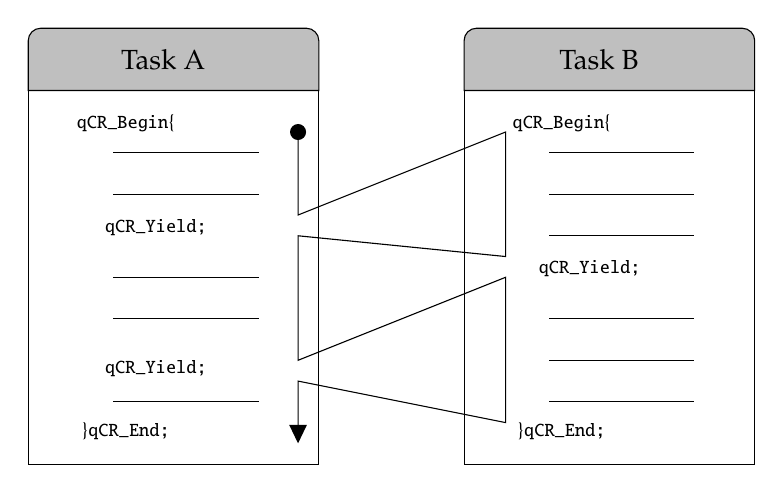
\begin{tikzpicture}[x=0.75pt,y=0.75pt,yscale=-1,xscale=1,scale=1]
        \foreach \x in {100,120,160,180,220}{ \draw    (121,\x) -- (191,\x) ; }
        \foreach \x in {100,120,140,180,200,220}{ \draw    (331,\x) -- (401,\x) ; }
        \draw   (290,70) -- (430,70) -- (430,250) -- (290,250) -- cycle ;
        \draw   (80,70) -- (220,70) -- (220,250) -- (80,250) -- cycle ;
        
        \draw  [fill=lightgray  ,fill opacity=1 ] (290,46) .. controls (290,42.69) and (292.69,40) .. (296,40) -- (424,40) .. controls (427.31,40) and (430,42.69) .. (430,46) -- (430,70) .. controls (430,70) and (430,70) .. (430,70) -- (290,70) .. controls (290,70) and (290,70) .. (290,70) -- cycle ;
        \draw  [fill=lightgray  ,fill opacity=1 ] (80,46) .. controls (80,42.69) and (82.69,40) .. (86,40) -- (214,40) .. controls (217.31,40) and (220,42.69) .. (220,46) -- (220,70) .. controls (220,70) and (220,70) .. (220,70) -- (80,70) .. controls (80,70) and (80,70) .. (80,70) -- cycle ;
        \draw    (210,90) -- (210,130) -- (310,90) -- (310,150) -- (210,140) -- (210,200) -- (310,160) -- (310,230) -- (210,210) -- (210,238) ;
        \draw [shift={(210,240)}, rotate = 270] [fill=black  ][line width=0.75]  [draw opacity=0] (8.93,-4.29) -- (0,0) -- (8.93,4.29) -- cycle    ;
        \draw [shift={(210,90)}, rotate = 90] [color=black  ][fill=black  ][line width=0.75]      (0, 0) circle [x radius= 3.35, y radius= 3.35]   ;
        \draw (145,55) node  [align=left] {Task A};
        \draw (127,86) node [scale=0.7, font=\ttfamily] [align=left] {\ttfamily{qCR_Begin\{}};
        \draw (127,234) node [scale=0.7] [align=left] {\ttfamily{\}qCR_End;}};
        \draw (141.5,136) node [scale=0.7] [align=left] {\ttfamily{qCR_Yield;}};
        \draw (141.5,204) node [scale=0.7] [align=left] {\ttfamily{qCR_Yield;}};
        \draw (355,55) node  [align=left] {Task B};
        \draw (337,86) node [scale=0.7] [align=left] {\ttfamily{qCR_Begin\{}};
        \draw (337,234) node [scale=0.7] [align=left] {\ttfamily{\}qCR_End;}};
        \draw (350.5,156) node [scale=0.7] [align=left] {\ttfamily{qCR_Yield;}};
    \end{tikzpicture}
    \caption{Coroutines in QuarkTS}
    \label{fig:coroutine}
\end{figure}
    
The QuarkTS implementation uses the Duff's device approach, and is heavily inspired by the Simon Tatham's Co-Routines in C \cite{tatham} and Adam Dunkels Protothreads \cite{dunkels}. This means that a \textit{local-continuation} variable is used to preserve the current state of execution at a particular place of the Co-Routine scope but without any call history or local variables. This brings benefits to lower RAM usage, but at the cost of some restrictions on how a Co-routine can be used. \\

\textbf{Limitations and Restrictions}:

\begin{itemize}
    \item The stack of a Co-Routine  is not maintained when a Co-Routine  yields. This means variables allocated on the stack will loose their values. To overcome this, a variable that must maintain its value across a blocking call must be declared as \lstinline{static}.
    \item Calls to API functions that could cause the Co-Routine to block, can only be made from the Co-Routine  function itself - not from within a function called by the Co-Routine .
    \item The implementation does not permit yielding or blocking calls to be made from within a \lstinline{switch} statement.
\end{itemize}

\subsubsection{Coding a Co-Routine}
The application writer just needs to create the body of the Co-Routine . This means starting a Co-Routine segment with \lstinline{qCR_Begin} \index{\lstinline{qCR_Begin}} and end with \lstinline{qCR_End} statement \index{\lstinline{qCR_End}}. From now on, yields and blocking calls from the Co-Routine scope are allowed. \\

\begin{lstlisting}[style=CStyle]
void CoroutineTask_Callback( qEvent_t e ){
    qCR_Begin{        
        if( EventNotComing() ){
            qCR_Yield;
        }
        DoTheEventProcessing();
    }qCR_End;
}
\end{lstlisting}   

A \lstinline{qCR_Yield} \index{\lstinline{qCR_Yield}} call return the CPU control back to the scheduler but saving the execution progress. With the next task activation, the Co-Routine will resume the execution after the last \lstinline{qCR_Yield} statement. \\

\begin{tcolorbox}
\HandRight All the Co-routine statements the \textit{qCR} appended at the beginning of their name.
\end{tcolorbox}

\begin{tcolorbox}
\HandRight Co-Routine statements can only be invoked from the scope of the Co-Routine.
\end{tcolorbox}


\subsubsection{Blocking calls}
Blocking calls inside a Co-Routine should be made with the provided statements, all of them with a common feature: an implicit yield.

A widely used procedure is to wait for a fixed period of time. For this, the \lstinline{qCR_Delay()} should be used \index{\lstinline{qCR_Delay}}. 

\begin{lstlisting}[style=CStyle]
qCR_Delay( qTime_t tDelay ) 
\end{lstlisting}

As expected, this statement makes an apparent blocking over the application flow, but to be precise, a yield is performed until the requested time expires, this allows other tasks to be executed until the blocking call finish. This \textit{"yielding until condition meet"} behavior its the common pattern among the other blocking statements. \\

Another common blocking call is \lstinline{qCR_WaitUntil()} \index{\lstinline{qCR_WaitUntil}}:

\begin{lstlisting}[style=CStyle]
qCR_WaitUntil( Condition ) 
\end{lstlisting}

This statement takes a \lstinline{Condition} argument, a logical expression that will be performed when the Co-Routine resumes their execution. As mentioned before, this type of statement exposes the expected behavior, yielding until the condition is met. \\


Optionally, the \lstinline{Do-Until} \index{\lstinline{qCR_Do}} \index{\lstinline{qCR_Until}} structure are also provided to perform a multi-line job before the yield, allowing more complex actions to be performed after the Co-Routine  resumes: \\

\begin{lstlisting}[style=CStyle]
qCR_Do{
    /* Job : a set of instructions*/
}qCR_Until( Condition );
\end{lstlisting}

\subsubsection*{Usage example:}
\begin{lstlisting}[style=CStyle]
void Sender_Task( qEvent_t e ){
    static qSTimer_t timeout;
    qCR_Begin{                  
        Send_Packet();
        /* 
           Wait until an acknowledgment has been received, or until
           the timer expires. If the timer expires, we should send
           the packet again. 
        */
        qSTimer_Set( &timeout, TIMEOUT_TIME );
        qCR_WaitUntil( PacketACK_Received() || 
                       qSTimer_Expired(&timeout));
    }qCR_End;
}

void Receiver_Task( qEvent_t e ){
    qCR_Begin{                  
        /* Wait until a packet has been received*/
        qCR_WaitUntil( Packet_Received() );
        Send_Acknowledgement();  
    }qCR_End;
}
\end{lstlisting} 

\subsubsection{Positional jumps}
This feature provides positional local jumps, control flow that deviates from the usual Co-Routine call. 

The complementary statements \lstinline{qCR_PositionGet()} \index{\lstinline{qCR_PositionGet}} and \lstinline{qCR_PositionRestore()} \index{\lstinline{qCR_PositionRestore}} provide this functionality.
The first one saves the Co-Routine state at some point of their execution into \lstinline{CRPos}, a variable of type \lstinline{qCR_Position_t} \index{\lstinline{qCR_Position_t}},  that can be used at some later point of program execution by \lstinline{qCR_PositionRestore()} to restore the Co-Routine  state to the one saved by \lstinline{qCR_PositionGet()} into \lstinline{CRPos}. This process can be imagined to be a "jump" back to the point of program execution where \lstinline{qCR_PositionGet()} saved the Co-Routine  environment. \\

\begin{lstlisting}[style=CStyle]
qCR_PositionGet( CRPos )
\end{lstlisting}

\begin{lstlisting}[style=CStyle]
qCR_PositionRestore( CRPos )
\end{lstlisting}

And to reset the \lstinline{CRPos} variable to the beginning of the Co-Routine, use \index{\lstinline{qCR_PositionReset}}:

\begin{lstlisting}[style=CStyle]
qCR_PositionReset( CRPos )
\end{lstlisting}

\subsubsection{Semaphores}
This module implements counting semaphores on top of Co-Routines. Semaphores are a synchronization primitive that provide two operations: \textit{wait} and \textit{signal}. The \textit{wait} operation checks the semaphore counter and blocks the Co-Routine if the counter is zero. The \textit{signal} operation increases the semaphore counter but does not block. If another Co-Routine has blocked waiting for the semaphore that is signaled, the blocked Co-Routines will become runnable again.

Semaphores are referenced by handles, a variable of type \lstinline{qCR_Semaphore_t} \index{\lstinline{qCR_Semaphore_t}}and must be initialized with \lstinline{qCR_SemInit()} \index{\lstinline{qCR_SemInit}} before any usage.  Here, a value for the counter is required. Internally, semaphores use an \lstinline{unsigned int} to represent the counter, therefore the \lstinline{Value} argument should be within range of this data-type. \\

\begin{lstlisting}[style=CStyle]
qCR_SemInit( sem, Value )
\end{lstlisting}

To perform the \textit{wait} operation, the \lstinline{qCR_SemWait()} \index{\lstinline{qCR_SemWait}} statement should be used. The wait operation causes the Co-routine to block while the counter is zero. When the counter reaches a value larger than zero, the Co-Routine will continue. \\


\begin{lstlisting}[style=CStyle]
qCR_SemWait( sem )
\end{lstlisting}

Finally, \lstinline{qCR_SemSignal()} \index{\lstinline{qCR_SemSignal}} carries out the \textit{signal} operation on the semaphore. This signaling increments the counter inside the semaphore, which eventually will cause waiting Co-routines to continue executing. \\

\begin{lstlisting}[style=CStyle]
qCR_SemSignal( sem )
\end{lstlisting}


\subsubsection*{Usage example:}
The following example shows how to implement the bounded buffer problem using Co-Routines and semaphores. The example uses two tasks: one that produces items and other that consumes items.

Note that there is no need for a mutex to guard the \lstinline{add_to_buffer()} and \lstinline{get_from_buffer()} functions because of the implicit locking semantics of Co-Routines, so it will never be preempted and will never block except in an explicit \lstinline{qCR_SemWait} statement. \\

\begin{lstlisting}[style=CStyle]
#include "HAL.h"
#include "QuarkTS.h"
#include "AppLibrary.h"

#define NUM_ITEMS 32
#define BUFSIZE 8

qTask_t ProducerTask, ConsumerTask;
qCR_Semaphore_t mutex, full, empty;
/*===================================================================*/
void ProducerTask_Callback( qEvent_t e ){
  static int produced;
  
  qCR_Begin{
     for(produced = 0; produced < NUM_ITEMS; ++produced) {
        qCR_SemWait( &full );
        qCR_SemWait( &mutex );

        add_to_buffer( produce_item() );  
  
        qCR_SemSignal( &mutex );
        qCR_SemSignal( &empty );
     }
  }qCR_End;
}
/*===================================================================*/
void ConsumerTask_Callback( qEvent_t e ){{
  static int consumed;
  
  qCR_Begin{
      for(consumed = 0; consumed < NUM_ITEMS; ++consumed) {
        qCR_SemWait( &empty );
        qCR_SemWait( &mutex );    

        consume_item( get_from_buffer() );    

        qCR_SemSignal( &mutex ); 
        qCR_SemSignal( &full );
      }
  }qCR_End;
}
/*===================================================================*/
void IdleTask_Callback( qEvent_t e ){
    /*nothing to do*/
} 
/*===================================================================*/
int main(void){ 
  HAL_Init();

  qOS_Setup( HAL_GetTick, 0.001, IdleTask_Callback );
  qCR_SemInit( &empty, 0 );
  qCR_SemInit( &full, BUFSIZE );
  qCR_SemInit( &mutex, 1 );	
  
  qOS_Add_Task( &ProducerTask, ProducerTask_Callback,
                qMedium_Priority, 0.1, qPeriodic, qEnabled, NULL );
  qOS_Add_Task( &ConsumerTask, ConsumerTask_Callback,
                qMedium_Priority, 0.1, qPeriodic, qEnabled, NULL );
  qOS_Run(); 	
  return 0;
}
\end{lstlisting}

\subsection{AT Command Line Interface} 
A command-line interface (CLI) is a way to interact directly with the software of an embedded system in the form of text commands and responses. It can be seen as a typed set of commands to produce a result, but here, the commands are typed in real-time by a user through a specific interface, for example, UART, USB, LAN, etc. 

A CLI is often developed to aid initial driver development and debugging. This CLI might become the interface (or one of the interfaces) used by a sophisticated end-user to interact with the product. Think of typing commands to control a machine, or perhaps for low-level access to the control system as a development tool, tweaking time-constants and monitoring low-level system performance during testing. 


\subsubsection{The components of the CLI}
The provided development API parses and handles input commands, following a simplified form of the extended AT-commands syntax. 

\begin{figure}[H]
    \centering
    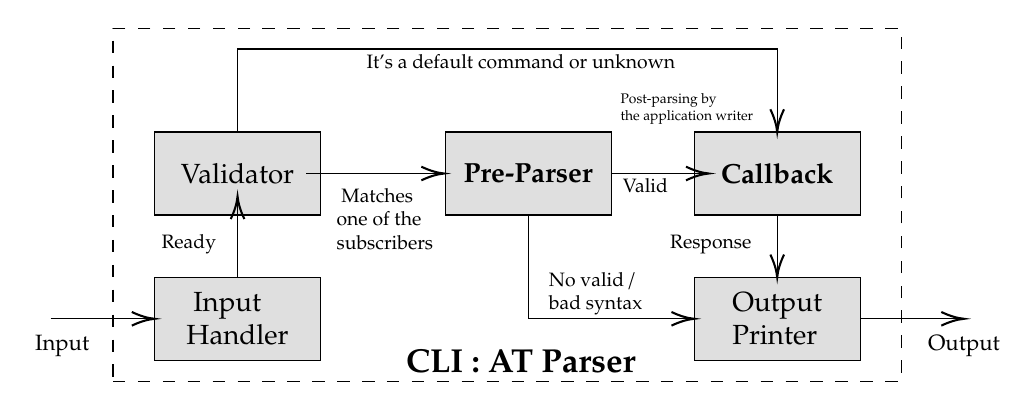
\begin{tikzpicture}[x=0.75pt,y=0.75pt,scale=1]
        \draw  [color=black  ,draw opacity=1 ][fill=white  ,fill opacity=1 ][dash pattern={on 4.5pt off 4.5pt}] (80,70) -- (460,70) -- (460,240) -- (80,240) -- cycle ;
        \draw  [fill=lightgray!50  ,fill opacity=1 ] (100,80) -- (180,80) -- (180,120) -- (100,120) -- cycle ;
        \draw  [fill=lightgray!50  ,fill opacity=1 ] (100,150) -- (180,150) -- (180,190) -- (100,190) -- cycle ;
        \draw  [fill=lightgray!50  ,fill opacity=1 ] (240,150) -- (320,150) -- (320,190) -- (240,190) -- cycle ;
        \draw  [fill=lightgray!50  ,fill opacity=1 ] (360,150) -- (440,150) -- (440,190) -- (360,190) -- cycle ;
        \draw  [fill=lightgray!50  ,fill opacity=1 ] (360,80) -- (440,80) -- (440,120) -- (360,120) -- cycle ;
        \draw    (140,190) -- (140,230) -- (400,230) -- (400,192) ;
        \draw [shift={(400,190)}, rotate = 450] [color=black ][line width=0.75]    (10.93,-3.29) .. controls (6.95,-1.4) and (3.31,-0.3) .. (0,0) .. controls (3.31,0.3) and (6.95,1.4) .. (10.93,3.29)   ;
        \draw    (50,100) -- (98,100) ;
        \draw [shift={(100,100)}, rotate = 180] [color=black ][line width=0.75]    (10.93,-3.29) .. controls (6.95,-1.4) and (3.31,-0.3) .. (0,0) .. controls (3.31,0.3) and (6.95,1.4) .. (10.93,3.29)   ;
        \draw    (440,100) -- (488,100) ;
        \draw [shift={(490,100)}, rotate = 180] [color=black ][line width=0.75]    (10.93,-3.29) .. controls (6.95,-1.4) and (3.31,-0.3) .. (0,0) .. controls (3.31,0.3) and (6.95,1.4) .. (10.93,3.29)   ;
        \draw    (400,150) -- (400,122) ;
        \draw [shift={(400,120)}, rotate = 450] [color=black ][line width=0.75]    (10.93,-3.29) .. controls (6.95,-1.4) and (3.31,-0.3) .. (0,0) .. controls (3.31,0.3) and (6.95,1.4) .. (10.93,3.29)   ;
        \draw    (280,150) -- (280,100) -- (358,100) ;
        \draw [shift={(360,100)}, rotate = 180] [color=black ][line width=0.75]    (10.93,-3.29) .. controls (6.95,-1.4) and (3.31,-0.3) .. (0,0) .. controls (3.31,0.3) and (6.95,1.4) .. (10.93,3.29)   ;
        \draw (400,170) node  [align=left] {\textbf{Callback}};
        \draw (280,170) node  [align=left] {\textbf{Pre-Parser}};
        \draw (140,170) node  [align=left] {Validator};
        \draw (400,100) node  [align=left] {Output\\Printer};
        \draw (140,100) node  [align=left] { \ Input\\Handler};
        \draw (55.5,87) node [scale=0.8] [align=left] {Input};
        \draw (490,87) node [scale=0.8] [align=left] {Output};
        \draw (368,136) node [scale=0.7] [align=left] {Response};
        \draw (336.5,164) node [scale=0.7] [align=left] {Valid};
        \draw (211,148) node [scale=0.7] [align=left] { \ Matches\\ one of the\\subscribers};
        \draw (276.5,224) node [scale=0.7] [align=left] {It's a default command or unknown};
        \draw (312.5,112) node [scale=0.7] [align=left] {No valid /\\bad syntax};
        \draw (356.5,201) node [scale=0.5] [align=left] {Post-parsing by \\the application writer};
        \draw (116.5,136) node [scale=0.7] [align=left] {Ready};
        \draw (276.5,79.5) node [scale=1.2] [align=left] {\textbf{CLI : AT Parser}};
        \draw    (173,170) -- (237.5,170) ;
        \draw [shift={(239.5,170)}, rotate = 180] [color=black ][line width=0.75]    (10.93,-3.29) .. controls (6.95,-1.4) and (3.31,-0.3) .. (0,0) .. controls (3.31,0.3) and (6.95,1.4) .. (10.93,3.29)   ;
        \draw    (320.5,170) -- (365,170) ;
        \draw [shift={(367,170)}, rotate = 180] [color=black ][line width=0.75]    (10.93,-3.29) .. controls (6.95,-1.4) and (3.31,-0.3) .. (0,0) .. controls (3.31,0.3) and (6.95,1.4) .. (10.93,3.29)   ;
        \draw    (140,120) -- (140,157) ;
        \draw [shift={(140,159)}, rotate = 270] [color=black ][line width=0.75]    (10.93,-3.29) .. controls (6.95,-1.4) and (3.31,-0.3) .. (0,0) .. controls (3.31,0.3) and (6.95,1.4) .. (10.93,3.29)   ;
    \end{tikzpicture}
    \caption{AT parser for a CLI implementation}
    \label{fig:atparser}
\end{figure}

As seen in figure \ref{fig:atparser}, the CLI has a few components described below:
\begin{itemize}
    \item  \textit{Input Handler} : It is responsible for collecting incoming data from the \textit{input} in the form of ASCII characters inside a buffer. When this buffer is ready by receiving an \lstinline{EOL}(\textit{End-Of-Line}) byte, it notifies the \textit{validator} to perform the initial checks.
    \item \textit{Validator}: Take the input string and perform three checks over it:
    \begin{enumerate}
        \item The input matches one of the subscribed commands.
        \item The input matches one of the default commands.
        \item The input is unknown
    \end{enumerate}
    \item \textit{Pre-Parser}: Takes the input if the \textit{validator} asserts the first check. It is responsible for syntax validation and classification. Also, prepares the input argument for the next component.
    \item \textit{Callback or Post-Parser}: If input at the \textit{pre-parser} is valid, the respective command-callback is invoked. Here, the application writer is free to handle the command execution and the output response.
    \item \textit{Output printer} : Takes all the return status of the previous components to print out a response at the output.
\end{itemize}

\begin{tcolorbox}
\HandRight Here, \textit{Input} and \textit{Output} should be provided by the application writer, for example, if a UART interface is chosen, the input should take the received bytes from an ISR and the output is a function to print out a single byte.
\end{tcolorbox}

\subsubsection{Supported syntax} \label{atsyntax}

The syntax is straightforward and the rules are provided below:

\begin{itemize}
    \item All command lines must start with \lstinline{AT} and end with an \lstinline{EOL} character. By default, the CLI uses the carriage return character. (We will use \lstinline{<CR>} to represent a carriage return character in this document).
    \item AT commands are case-insensitive 
    \item Only four types of AT commands are allowed:
    \begin{itemize}
        \item \textbf{Acting} (\lstinline{QATCLI_CMDTYPE_ACT}) : This is the simplest type of commands that can be subscribed. Its normally used to execute the action that the command should do. This type doesn't take arguments or modifiers, for example,
        \begin{lstlisting}
        AT+CMD
        \end{lstlisting}
        \item \textbf{Read} (\lstinline{QATCLI_CMDTYPE_READ}) : This type of command allows you to read or test a value already configured for the specified parameter. Only one argument is allowed.
        \begin{lstlisting}
        AT+CMD?
        AT+CMD?PARAM1
        \end{lstlisting}        
        \item \textbf{Test} (\lstinline{QATCLI_CMDTYPE_TEST}) : These types of commands allow you to get the values that can be set for its parameters. No parameters are allowed here.
        \begin{lstlisting}
        AT+CMD=?
        \end{lstlisting}
        \item \textbf{Parameter Set} (\lstinline{QATCLI_CMDTYPE_PARA}) : These types of commands allow \textit{n} arguments to be passed for setting parameters, for example:
        \begin{lstlisting}
        AT+CMD=x,y
        \end{lstlisting}
    \end{itemize}
    If none of the types is given at the input, the command response will be \lstinline{ERROR}
    \item The possible output responses are:
    \begin{itemize}
        \item \lstinline{OK}: Indicates the successful execution of the command.
        \item \lstinline{ERROR}: A generalized message to indicate failure in executing the command. 
        \item \lstinline{UNKNOWN} : The input command its not subscribed.
        \item \lstinline{NOT ALLOWED} : The command syntax is not one of the allowed types.
        \item \lstinline{User-defined}: A custom output message defined by the application writer.
        \item \lstinline{NONE} : No response.
    \end{itemize}
\end{itemize}

All responses are followed by a \lstinline{<CR><LF>}. \\

Errors generated during the execution of these AT commands could be due to the following reasons:
\begin{itemize}
    \item Incorrect syntax/parameters of the AT command
    \item Bad parameters or not allowed operations defined by the application writer.
\end{itemize}

In case of an error, the string \lstinline{ERROR} or \lstinline{ERROR:<error_no>} are displayed.

\subsubsection{Setting up an AT-CLI instance}
Before starting the CLI development, the corresponding instance must be defined; a data structure of type \lstinline{qATCLI_t} \index{\lstinline{qATCLI_t}}. 
The instance should be initialized using the \lstinline{qATCLI_Setup()} API \index{\lstinline{qATCLI_Setup}}.

A detailed description of this function is shown bellow:  \\

\begin{lstlisting}[style=CStyle]
qBool_t qATCLI_Setup( qATCLI_t * const cli, const qPutChar_t OutputFcn, 
                      char *Input, const size_t SizeInput, char *Output, 
                      const size_t SizeOutput, const char *Identifier, 
                      const char *OK_Response, const char *ERROR_Response, 
                      const char *NOTFOUND_Response, const char *term_EOL )
\end{lstlisting}

\subsubsection*{Parameters}
\begin{itemize}
    \item \lstinline{cli} : A pointer to the AT Command Line Interface instance. 
    \item \lstinline{OutputFcn} : The basic output-char wrapper function. All the parser responses  will be printed-out through this function.
    \item \lstinline{Input} : A memory location to store the parser input (mandatory) 
    \item \lstinline{SizeInput} : The size of the memory allocated in \lstinline{Input}. 
    \item \lstinline{Output} : A memory location to store the parser output. If not used, pass \lstinline{NULL}.
    \item \lstinline{SizeOutput} : The size of the memory allocated in \lstinline{Output}. 
    \item \lstinline{Identifier} : The device identifier string. This string will be printed-out after a call to the \lstinline{AT_DEFAULT_ID_COMMAND}.
    \item \lstinline{OK_Response} : The output message when a command callback returns \lstinline{QATCLI_OK}. To use the default, pass \lstinline{NULL}.
    \item \lstinline{ERROR_Response} : The output message when a command callback returns \lstinline{QATCLI_ERROR} or any \lstinline{QATCLI_ERRORCODE(#)}. To use the default, pass \lstinline{NULL}.
    \item \lstinline{NOTFOUND_Response } : The output message when input doesn't match with any of  the available commands. To use the default, pass \lstinline{NULL}.
    \item \lstinline{term_EOL} : The \textit{End-Of-Line} string printed out after any of the parser messages. To use the default, pass \lstinline{NULL}. 
\end{itemize}

\subsubsection{Subscribing commands to the parser}
The AT CLI is able to subscribe any number of custom AT commands. For this, the 
\lstinline{qATCLI_CmdSubscribe()} \index{\lstinline{qATCLI_CmdSubscribe}} API should be used.

This function subscribes the CLI instance to a specific command with an associated callback function, so that next time the required command is sent to the CLI input, the callback function will be executed. \\
The CLI module only analyzes commands that follow the simplified AT-Commands syntax already described in section \ref{atsyntax}. \\

\begin{lstlisting}[style=CStyle]
qBool_t qATCLI_CmdSubscribe( qATCLI_t * const cli, 
                             qATCLI_Command_t * const Command, 
                             const char *TextCommand, 
                             qATCLI_CommandCallback_t Callback, 
                             qATCLI_Options_t CmdOpt, void *param )
\end{lstlisting}

\subsubsection*{Parameters}
\begin{itemize}
    \item \lstinline{cli} : A pointer to the AT Command Line Inteface instance. 
    \item \lstinline{Command} :  A pointer to the AT command object.
    \item \lstinline{TextCommand} : The string (name) of the command we want to subscribe to. Since this service only handles AT commands, this string has to begin by the \lstinline{"at"} characters and should be in lower case.
    \item \lstinline{Callback} : The handler of the callback function associated to the command. Prototype: 
    \lstinline{qATCLI_Response_t xCallback(qATCLI_Handler_t, qATCLI_PreCmd_t )}
    \item \lstinline{CmdOpt} : This flag combines with a bitwise ‘OR’ (‘|’) the following information:
    \begin{itemize}
        \item \lstinline{QATCLI_CMDTYPE_PARA} : \lstinline{AT+cmd=x,y} is allowed. The execution of the callback function also depends on whether the number of argument is valid or not. Information about number of arguments is combined with a bitwise 'OR' : \lstinline{QATCLI_CMDTYPE_PARA | 0xXY} , where \lstinline{X} which defines maximum argument number for incoming command and \lstinline{Y} which defines minimum argument number for incoming command.
        \item \lstinline{QATCLI_CMDTYPE_TEST} : \lstinline{AT+cmd=?} is allowed. 
        \item \lstinline{QATCLI_CMDTYPE_READ} : \lstinline{AT+cmd?} is allowed. 
        \item \lstinline{QATCLI_CMDTYPE_ACT} : \lstinline{AT+cmd} is allowed. 
    \end{itemize}
    \item \lstinline{param} :  User storage pointer.
\end{itemize}

\subsubsection{Writing a command callback}
The command callback should be coded by the application writter. Here, the following prototype should be used: \\

\begin{lstlisting}[style=CStyle]
qATCLI_Response_t CMD_Callback( qATCLI_Handler_t h, qATCLI_PreCmd_t p ){
    
}
\end{lstlisting}

The callback takes two arguments and returns a single value. The first argument is just a pointer to public data of the parser instance where the command it subscribed. From the callback context, it can be used to print out extra information as a command response. \\

The second one is the main parameter from the point of view of the application writer, and correspond to a handle of type \lstinline{qATCLI_PreCmd_t} \index{\lstinline{qATCLI_PreCmd_t}}. The members inside points to data filled by the Pre-Parser component to give information about the detected command, like the type, number of arguments and the subsequent string after the command text.The pointed members are described as follows:

\begin{itemize}
    \item \lstinline{Command} : A pointer to the calling AT Command object.
    \item \lstinline{Type} : The command type.
    \item \lstinline{StrData} : The string data after the command text.
    \item \lstinline{StrLen} : The length of \lstinline{StrData}.
    \item \lstinline{NumArgs} : Number of arguments, only available if \lstinline{Type = QATCLI_CMDTYPE_PARA}.
\end{itemize}

The return value (an enum of type \lstinline{qATCLI_Response_t}) \index{\lstinline{qATCLI_Response_t}} determines the response shown by the \textit{Output printer} component. The possible allowed values are:

\begin{itemize}
    \item \lstinline{QATCLI_OK} : as expected, print out the \lstinline{OK} string.
    \item \lstinline{QATCLI_ERROR} : as expected, print out the \lstinline{ERROR} string.
    \item \lstinline{QATCLI_ERRORCODE(no)} : Used to indicate an error code. This code is defined by the application writer and should be a value between 1 and 32766. For example, a return value of \lstinline{QATCLI_ERRORCODE(15)}, will print out the string \lstinline{ERROR:15}.
    \item \lstinline{QATCLI_NORESPONSE} : No response will be printed out.
\end{itemize}


A simple example of how the command callback should be coded is showed below: \\

\begin{lstlisting}[style=CStyle]
qATCLI_Response_t CMD_Callback( qATCLI_Handler_t h, qATCLI_PreCmd_t p ){
	qATCLI_Response_t Response = QATCLI_NORESPONSE;
	switch(param->Type){
		case QATCLI_CMDTYPE_PARA:
			Response = QATCLI_OK;
			break;
		case QATCLI_CMDTYPE_TEST:
			Response = QATCLI_OK;
			break;
		case QATCLI_CMDTYPE_READ:
		    strcpy( h->Output , "Test");
			Response = QATCLI_OK;
			break;
		case QATCLI_CMDTYPE_ACT:
			Response = QATCLI_OK;
			break;			
		default:
			Response = QATCLI_ERROR;
			break;
	}
	return Response;
}
\end{lstlisting}


\subsubsection{Handling the input}
Input handling is simplified using the provided APIs. The \lstinline{qATCLI_ISRHandler()} \index{\lstinline{qATCLI_ISRHandler}} and \lstinline{qATCLI_ISRHandlerBlock()}  \index{\lstinline{qATCLI_ISRHandlerBlock}} functions are intended to be used from the interrupt context. This avoids any kind of polling implementation and allows the CLI application to be designed using an event-driven pattern.

\begin{lstlisting}[style=CStyle]
qBool_t qATCLI_ISRHandler( qATCLI_t * const cli, char c )
\end{lstlisting}

\begin{lstlisting}[style=CStyle]
qBool_t qATCLI_ISRHandlerBlock( qATCLI_t * const cli, char *data, 
                                const size_t n )
\end{lstlisting}

Both functions feed the parser input, the first one with a single character and the second with a string. The application writer should call one of these functions from the desired hardware interface, for example, from a UART receive ISR. 

\subsubsection*{Parameters}
\begin{itemize}
    \item \lstinline{cli} : Both APIs take a pointer to AT Command Line Interface instance.
\end{itemize}

for \lstinline{qATCLI_ISRHandler} :
\begin{itemize}
    \item \lstinline{c} : The incoming byte/char to the input. 
\end{itemize}

for \lstinline{qATCLI_ISRHandlerBlock} :
\begin{itemize}
    \item \lstinline{data} : The incoming string.
    \item \lstinline{n} : The length of the \lstinline{data} argument.
\end{itemize}

\subsubsection*{Return Value}
\lstinline{qTrue} when the CLI is ready to process the input, otherwise return \lstinline{qFalse}.

\noindent\hrulefill
\newline
If there are no intention to feed the input from the ISR context, the APIs \lstinline{qATCLI_Raise} \index{\lstinline{qATCLI_Raise}} or \lstinline{qATCLI_Exec} \index{\lstinline{qATCLI_Exec}} can be called at demand from the base context. \\

\begin{lstlisting}[style=CStyle]
qBool_t qATCLI_Raise( qATCLI_t * const cli, const char *cmd )
\end{lstlisting}

\begin{lstlisting}[style=CStyle]
qATCLI_Response_t qATCLI_Exec( qATCLI_t * const cli, const char *cmd )
\end{lstlisting}

As expected, both functions send the string to the specified CLI.
The difference between both APIs is that \lstinline{qATCLI_Raise()} sends the command through the input, marking it as ready for parsing and acting as the \textit{Input handler} component.
The \lstinline{qATCLI_Exec()}, on the other hand, executes the components of \textit{Pre-parsing} and \textit{Post-parsing} bypassing the other components, including the \textit{Output printer}, so that it must be handled by the application writer.

\subsubsection*{Parameters:}
\begin{itemize}
    \item \lstinline{cli} : A pointer to the AT Command Line Inteface instance.
    \item \lstinline{cmd} : The command string, including arguments if required.
\end{itemize}

\subsubsection*{Return value:}
For \lstinline{qATCLI_Raise()}, \lstinline{qTrue} if the command was successfully raised, otherwise returns \lstinline{qFalse}.

For \lstinline{qATCLI_Exec()}, the same value returned by the respective callback function. If the input string doesn't match any of the subscribed commands, returns \lstinline{QAT_NOTFOUND}. If the input syntax is not allowed, returns \lstinline{qAT_NOTALLOWED}. \\

\begin{tcolorbox}
\ArrowBoldDownRight \textit{Note}: All functions involved with the component \textit{Input-handler},  ignores non-graphic characters and cast any uppercase to lowercase.
\end{tcolorbox}

\subsubsection{Running the parser} \label{runningparser}
The parser can be invoked directly using the \lstinline{qATCLI_Run()} \index{\lstinline{qATCLI_Run}} API. Almost all the components that make up the CLI are performed by this API, except for the \textit{Input Handler}, that should be managed by the application writer itself. \\

\begin{lstlisting}[style=CStyle]
qBool_t qATCLI_Run( qATCLI_t * const Parser )
\end{lstlisting}

In this way, the writer of the application must implement the logic that leads this function to be called when the \textit{input-ready} condition is given.

The simple approach for this is to check the return value of any of the input feeder APIs and set a notification variable when they report a ready input. Later in the base context, a polling job should be performed over this notification variable, running the parser when their value is true, then clearing the value after to avoid unnecessary overhead. 

The recommended implementation is to leave this job be handled by a task instead of coding the logic to know when the CLI should run. For this, the \lstinline{qOS_Add_ATCLITask()} is provided. This API \index{\lstinline{qOS_Add_ATCLITask}} add a task to the scheduling scheme running an AT Command Line Interface and treated as an event-triggered task. The address of the parser instance will be stored in the \lstinline{TaskData} storage-Pointer. \\

\begin{lstlisting}[style=CStyle]
qBool_t qOS_Add_ATCLITask( qTask_t * const Task, 
                           qATCLI_t *cli, 
                           qPriority_t Priority )
\end{lstlisting}

\subsubsection*{Parameters}
\begin{itemize}
    \item \lstinline{Task} : A pointer to the task node. 
    \item \lstinline{Parser} :  A pointer to the AT Command Line Interface instance.
    \item \lstinline{Priority} : Task priority Value. [0(min) - \lstinline{Q_PRIORITY_LEVELS}(max)]
\end{itemize}

After invoked, both CLI and task are linked together in such a way that when an \textit{input-ready} condition is given, a notification event is sent to the task launching the CLI components. As the task is event-triggered, there is no additional overhead and the writer of the application can assign a priority value to balance the application against other tasks in the scheduling scheme.

\subsubsection{Retrieving arguments inside a command-callback}

The following APIs should be only invoked from a command-callback context: \\

\begin{lstlisting}[style=CStyle]
char* qATCLI_GetArgString( const qATCLI_PreCmd_t param, qINT8_t n,
                           char* out)
\end{lstlisting}

Get the argument parsed as string from the incoming AT command. \index{\lstinline{qATCLI_GetArgString}}

\subsubsection*{Parameters:}
\begin{itemize}
    \item \lstinline{param} : A handle to the pre-parser instance(only available from the AT-Command callback).
    \item \lstinline{n} : The number of the argument.
    \item \lstinline{out} :  Array in memory where to store the resulting null-terminated string.
\end{itemize}

\subsubsection*{Return value:}
Same as \lstinline{out} on success, otherwise returns \lstinline{NULL}.

\noindent\hrulefill
\newline
Next APIs takes the same arguments: \\

\begin{lstlisting}[style=CStyle]
char* qATCLI_GetArgPtr( const qATCLI_PreCmd_t param, qINT8_t n )
\end{lstlisting}

To get the pointer where the desired argument starts. \index{\lstinline{qATCLI_GetArgPtr}}

\begin{lstlisting}[style=CStyle]
int qATCLI_GetArgInt( const qATCLI_PreCmd_t param, qINT8_t n )
\end{lstlisting}

To get the argument parsed as integer from the incoming AT command. \index{\lstinline{qATCLI_GetArgInt}}

\begin{lstlisting}[style=CStyle]
qFloat32_t qATCLI_GetArgFlt( const qATCLI_PreCmd_t param, qINT8_t n )
\end{lstlisting}

To get the argument parsed as float from the incoming AT command. \index{\lstinline{qATCLI_GetArgFlt}}

\begin{lstlisting}[style=CStyle]
qUINT32_t qATCLI_GetArgHex( const qATCLI_PreCmd_t param, qINT8_t n )
\end{lstlisting}

To get the HEX argument parsed as \lstinline{qUINT32_t} from the incoming AT command. \index{\lstinline{qATCLI_GetArgHex}}


\subsubsection*{Parameters:}
\begin{itemize}
    \item \lstinline{param} : A handle to the pre-parser instance(only available from the AT-Command callback).
    \item \lstinline{n} : The number of the argument.
\end{itemize}

\subsubsection*{Return value:}
For \lstinline{qATCLI_GetArgPtr()}, a pointer to the desired argument. \lstinline{NULL} pointer if the argument is not present. \\
For \lstinline{qATCLI_GetArgInt()}, the argument parsed as integer. Same behavior of \lstinline{qIOUtil_AtoI}. If argument not found returns 0.\\
For \lstinline{qATCLI_GetArgFlt()}, the argument parsed as \lstinline{float}. Same behavior of \lstinline{qIOUtil_AtoF}. If argument not found returns 0.\\
For \lstinline{qATCLI_GetArgHex()}, the HEX argument parsed as \lstinline{qUINT32_t}. Same behavior of \lstinline{qIOUtil_XtoU32}. If argument not found returns 0.

\subsection{Memory Management} \label{memmanagement}
Memory can be allocated using the standard C library malloc() and free() functions, but they may not be suitable in most embedded applications because they are not always available on small microcontrollers or their implementation can be relatively large, taking up valuable code space. Additionally, some implementations can suffer from fragmentation.

To get around this problem, the OS  provides its own memory allocation API. When the application requires RAM, instead of calling \textit{malloc()},  call \lstinline{qMalloc()} \index{\lstinline{qMalloc}}. When RAM is being freed, instead of calling \textit{free()}, use \lstinline{qFree()} \index{\lstinline{qFree}}. Both functions have the same prototype as the standard C library counterparts.

\subsubsection{Principle of operation}
The allocation scheme works by subdividing a static array into smaller blocks and using the \textit{First-Fit} approach (see figure \ref{fig:memman}). 

\begin{figure}[H]
    \centering
    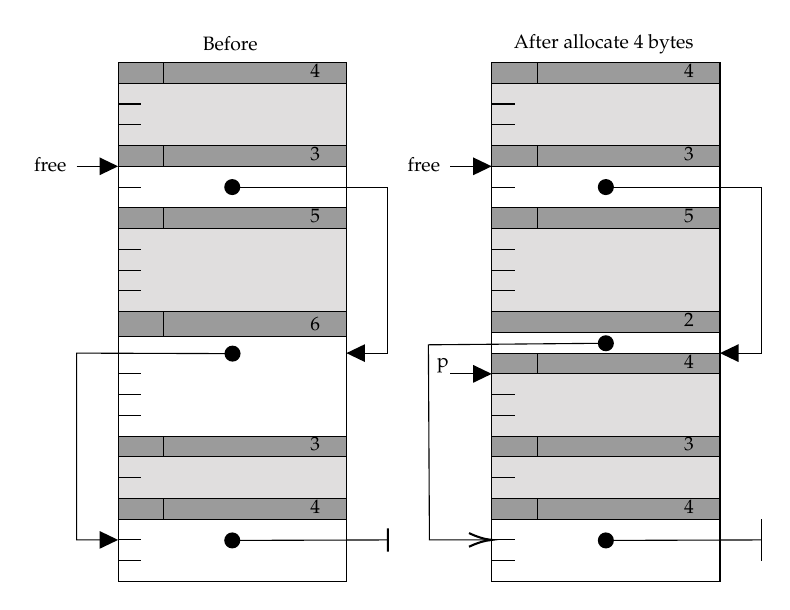
\begin{tikzpicture}[x=0.75pt,y=0.75pt,yscale=-1,xscale=1]
        \draw  [fill={rgb, 255:red, 155; green, 155; blue, 155 }  ,fill opacity=1 ] (100,20) -- (210,20) -- (210,30) -- (100,30) -- cycle ;
        \draw  [fill={rgb, 255:red, 224; green, 222; blue, 222 }  ,fill opacity=1 ] (100,30) -- (210,30) -- (210,60) -- (100,60) -- cycle ;
        \draw    (100,40) -- (111,40) ;
        \draw    (111,50) -- (100,50) ;
        \draw    (122,20) -- (122,30) ;
        \draw  [fill={rgb, 255:red, 155; green, 155; blue, 155 }  ,fill opacity=1 ] (100,60) -- (210,60) -- (210,70) -- (100,70) -- cycle ;
        \draw  [fill={rgb, 255:red, 255; green, 255; blue, 255 }  ,fill opacity=1 ] (100,70) -- (210,70) -- (210,90) -- (100,90) -- cycle ;
        \draw    (100,80) -- (111,80) ;
        \draw    (122,60) -- (122,70) ;
        \draw  [fill={rgb, 255:red, 224; green, 222; blue, 222 }  ,fill opacity=1 ] (100,100) -- (210,100) -- (210,140) -- (100,140) -- cycle ;
        \draw  [fill={rgb, 255:red, 155; green, 155; blue, 155 }  ,fill opacity=1 ] (100,90) -- (210,90) -- (210,100) -- (100,100) -- cycle ;
        \draw    (111,110) -- (100,110) ;
        \draw    (111,120) -- (100,120) ;
        \draw    (111,130) -- (100,130) ;
        \draw    (122,90) -- (122,100) ;
        \draw  [fill={rgb, 255:red, 255; green, 255; blue, 255 }  ,fill opacity=1 ] (100,152) -- (210,152) -- (210,200) -- (100,200) -- cycle ;
        \draw  [fill={rgb, 255:red, 155; green, 155; blue, 155 }  ,fill opacity=1 ] (100,140) -- (210,140) -- (210,152) -- (100,152) -- cycle ;
        \draw    (111,170) -- (100,170) ;
        \draw    (111,180) -- (100,180) ;
        \draw    (122,140) -- (122,152) ;
        \draw    (111,190) -- (100,190) ;
        \draw  [fill={rgb, 255:red, 155; green, 155; blue, 155 }  ,fill opacity=1 ] (100,200) -- (210,200) -- (210,210) -- (100,210) -- cycle ;
        \draw    (122,200) -- (122,210) ;
        \draw  [fill={rgb, 255:red, 224; green, 222; blue, 222 }  ,fill opacity=1 ] (100,210) -- (210,210) -- (210,230) -- (100,230) -- cycle ;
        \draw    (111,220) -- (100,220) ;
        \draw  [fill={rgb, 255:red, 155; green, 155; blue, 155 }  ,fill opacity=1 ] (100,230) -- (210,230) -- (210,240) -- (100,240) -- cycle ;
        \draw  [fill={rgb, 255:red, 255; green, 255; blue, 255 }  ,fill opacity=1 ] (100,240) -- (210,240) -- (210,270) -- (100,270) -- cycle ;
        \draw    (100,250) -- (111,250) ;
        \draw    (111,260) -- (100,260) ;
        \draw    (122,230) -- (122,240) ;
        \draw    (155,80) -- (230,80) -- (230,160) -- (212,160) ;
        \draw [shift={(210,160)}, rotate = 360] [fill={rgb, 255:red, 0; green, 0; blue, 0 }  ][line width=0.75]  [draw opacity=0] (8.93,-4.29) -- (0,0) -- (8.93,4.29) -- cycle    ;
        \draw [shift={(155,80)}, rotate = 0] [color={rgb, 255:red, 0; green, 0; blue, 0 }  ][fill={rgb, 255:red, 0; green, 0; blue, 0 }  ][line width=0.75]      (0, 0) circle [x radius= 3.35, y radius= 3.35]   ;
        \draw    (155.13,160.25) -- (80,160) -- (80,250) -- (98,250) ;
        \draw [shift={(100,250)}, rotate = 180] [fill={rgb, 255:red, 0; green, 0; blue, 0 }  ][line width=0.75]  [draw opacity=0] (8.93,-4.29) -- (0,0) -- (8.93,4.29) -- cycle    ;
        \draw [shift={(155.13,160.25)}, rotate = 180.19] [color={rgb, 255:red, 0; green, 0; blue, 0 }  ][fill={rgb, 255:red, 0; green, 0; blue, 0 }  ][line width=0.75]      (0, 0) circle [x radius= 3.35, y radius= 3.35]   ;
        \draw    (80,70) -- (98,70) ;
        \draw [shift={(100,70)}, rotate = 180] [fill={rgb, 255:red, 0; green, 0; blue, 0 }  ][line width=0.75]  [draw opacity=0] (8.93,-4.29) -- (0,0) -- (8.93,4.29) -- cycle    ;
        \draw    (155,250.25) -- (230,250) ;
        \draw [shift={(230,250)}, rotate = 539.81] [color={rgb, 255:red, 0; green, 0; blue, 0 }  ][line width=0.75]    (0,5.59) -- (0,-5.59)   ;
        \draw [shift={(155,250.25)}, rotate = 359.81] [color={rgb, 255:red, 0; green, 0; blue, 0 }  ][fill={rgb, 255:red, 0; green, 0; blue, 0 }  ][line width=0.75]      (0, 0) circle [x radius= 3.35, y radius= 3.35]   ;
        \draw  [fill={rgb, 255:red, 155; green, 155; blue, 155 }  ,fill opacity=1 ] (280,20) -- (390,20) -- (390,30) -- (280,30) -- cycle ;
        \draw  [fill={rgb, 255:red, 224; green, 222; blue, 222 }  ,fill opacity=1 ] (280,30) -- (390,30) -- (390,60) -- (280,60) -- cycle ;
        \draw    (280,40) -- (291,40) ;
        \draw    (291,50) -- (280,50) ;
        \draw    (302,20) -- (302,30) ;
        \draw  [fill={rgb, 255:red, 155; green, 155; blue, 155 }  ,fill opacity=1 ] (280,60) -- (390,60) -- (390,70) -- (280,70) -- cycle ;
        \draw  [fill={rgb, 255:red, 255; green, 255; blue, 255 }  ,fill opacity=1 ] (280,70) -- (390,70) -- (390,90) -- (280,90) -- cycle ;
        \draw    (280,80) -- (291,80) ;
        \draw    (302,60) -- (302,70) ;
        \draw  [fill={rgb, 255:red, 224; green, 222; blue, 222 }  ,fill opacity=1 ] (280,100) -- (390,100) -- (390,140) -- (280,140) -- cycle ;
        \draw  [fill={rgb, 255:red, 155; green, 155; blue, 155 }  ,fill opacity=1 ] (280,90) -- (390,90) -- (390,100) -- (280,100) -- cycle ;
        \draw    (291,110) -- (280,110) ;
        \draw    (291,120) -- (280,120) ;
        \draw    (291,130) -- (280,130) ;
        \draw    (302,90) -- (302,100) ;
        \draw  [fill={rgb, 255:red, 255; green, 255; blue, 255 }  ,fill opacity=1 ] (280,150) -- (390,150) -- (390,200) -- (280,200) -- cycle ;
        \draw  [fill={rgb, 255:red, 155; green, 155; blue, 155 }  ,fill opacity=1 ] (280,140) -- (390,140) -- (390,150) -- (280,150) -- cycle ;
        \draw  [fill={rgb, 255:red, 155; green, 155; blue, 155 }  ,fill opacity=1 ] (280,200) -- (390,200) -- (390,210) -- (280,210) -- cycle ;
        \draw    (302,200) -- (302,210) ;
        \draw  [fill={rgb, 255:red, 224; green, 222; blue, 222 }  ,fill opacity=1 ] (280,210) -- (390,210) -- (390,230) -- (280,230) -- cycle ;
        \draw    (291,220) -- (280,220) ;
        \draw  [fill={rgb, 255:red, 155; green, 155; blue, 155 }  ,fill opacity=1 ] (280,230) -- (390,230) -- (390,240) -- (280,240) -- cycle ;
        \draw  [fill={rgb, 255:red, 255; green, 255; blue, 255 }  ,fill opacity=1 ] (280,240) -- (390,240) -- (390,270) -- (280,270) -- cycle ;
        \draw    (280,250) -- (291,250) ;
        \draw    (291,260) -- (280,260) ;
        \draw    (302,230) -- (302,240) ;
        \draw    (335,80) -- (410,80) -- (410,160) -- (392,160) ;
        \draw [shift={(390,160)}, rotate = 360] [fill={rgb, 255:red, 0; green, 0; blue, 0 }  ][line width=0.75]  [draw opacity=0] (8.93,-4.29) -- (0,0) -- (8.93,4.29) -- cycle    ;
        \draw [shift={(335,80)}, rotate = 0] [color={rgb, 255:red, 0; green, 0; blue, 0 }  ][fill={rgb, 255:red, 0; green, 0; blue, 0 }  ][line width=0.75]      (0, 0) circle [x radius= 3.35, y radius= 3.35]   ;
        \draw    (260,70) -- (278,70) ;
        \draw [shift={(280,70)}, rotate = 180] [fill={rgb, 255:red, 0; green, 0; blue, 0 }  ][line width=0.75]  [draw opacity=0] (8.93,-4.29) -- (0,0) -- (8.93,4.29) -- cycle    ;
        \draw    (335,250.25) -- (410,250) ;
        \draw [shift={(335,250.25)}, rotate = 359.81] [color={rgb, 255:red, 0; green, 0; blue, 0 }  ][fill={rgb, 255:red, 0; green, 0; blue, 0 }  ][line width=0.75]      (0, 0) circle [x radius= 3.35, y radius= 3.35]   ;
        \draw    (410,240) -- (410,260) ;
        \draw  [fill={rgb, 255:red, 155; green, 155; blue, 155 }  ,fill opacity=1 ] (280,160) -- (390,160) -- (390,170) -- (280,170) -- cycle ;
        \draw  [fill={rgb, 255:red, 224; green, 222; blue, 222 }  ,fill opacity=1 ] (280,170) -- (390,170) -- (390,200) -- (280,200) -- cycle ;
        \draw    (280,180) -- (291,180) ; 
        \draw    (291,190) -- (280,190) ;
        \draw    (302,160) -- (302,170) ; 
        \draw    (260,170) -- (278,170) ;
        \draw [shift={(280,170)}, rotate = 180] [fill={rgb, 255:red, 0; green, 0; blue, 0 }  ][line width=0.75]  [draw opacity=0] (8.93,-4.29) -- (0,0) -- (8.93,4.29) -- cycle    ;
        \draw    (335,155.25) -- (249.5,156) -- (250,250) -- (278,250) ;
        \draw [shift={(280,250)}, rotate = 180] [color={rgb, 255:red, 0; green, 0; blue, 0 }  ][line width=0.75]    (10.93,-3.29) .. controls (6.95,-1.4) and (3.31,-0.3) .. (0,0) .. controls (3.31,0.3) and (6.95,1.4) .. (10.93,3.29)   ;
        \draw [shift={(335,155.25)}, rotate = 179.5] [color={rgb, 255:red, 0; green, 0; blue, 0 }  ][fill={rgb, 255:red, 0; green, 0; blue, 0 }  ][line width=0.75]      (0, 0) circle [x radius= 3.35, y radius= 3.35]   ;
        \draw (195,24) node [scale=0.7] [align=left] {4};
        \draw (195,64) node [scale=0.7] [align=left] {3};
        \draw (195,94) node [scale=0.7] [align=left] {5};
        \draw (195,146) node [scale=0.7] [align=left] {6};
        \draw (195,204) node [scale=0.7] [align=left] {3};
        \draw (195,234) node [scale=0.7] [align=left] {4};
        \draw (67.33,69.33) node [scale=0.7] [align=left] {free};
        \draw (375,24) node [scale=0.7] [align=left] {4};
        \draw (375,64) node [scale=0.7] [align=left] {3};
        \draw (375,94) node [scale=0.7] [align=left] {5};
        \draw (375,144) node [scale=0.7] [align=left] {2};
        \draw (375,204) node [scale=0.7] [align=left] {3};
        \draw (375,234) node [scale=0.7] [align=left] {4};
        \draw (247.33,69.33) node [scale=0.7] [align=left] {free};
        \draw (375,164) node [scale=0.7] [align=left] {4};
        \draw (256.5,166) node [scale=0.7] [align=left] {p};
        \draw (154,11) node [scale=0.7] [align=left] {Before};
        \draw (334,11) node [scale=0.7] [align=left] {After allocate 4 bytes};
    \end{tikzpicture}
    \caption{First-fit allocation policy}
    \label{fig:memman}
\end{figure}

If adjacent free blocks are available, the implementation combines them into a single larger block, minimizing the risk of fragmentation, making it suitable for applications that repeatedly allocate and free different sized blocks of RAM. \\

\begin{tcolorbox}
\ArrowBoldDownRight \textit{Note}: Because memory is statically declared, it will make the application appear to consume a lot of RAM, even before any memory has been allocated from it.
\end{tcolorbox}

\begin{tcolorbox}
\AsteriskBold \textit{Warning}: All the memory management APIs are NOT interrupt-safe. Use these APIs only from the base context.
\end{tcolorbox}

\subsubsection{Memory pools}

A memory pool is a kernel object that allows memory blocks to be dynamically allocated from a user-designated memory region. Instead of typical pools with fixed-size block allocation, the pools in QuarkTS can be of any size, thereby the user is responsible for selecting the appropriate memory pool to allocate data with the same size. 

The \textit{default} memory management unit resides in a memory pool object. Also called the \textit{default pool}. The total amount of available heap space in the default memory pool is set by \lstinline{Q_DEFAULT_HEAP_SIZE}, which is defined in \lstinline{qconfig.h}.

Besides the \textit{default} pool, any number of additional memory pools can be defined. Like any other kernel object in QuarkTS, memory pools are referenced by handles, a variable of type \lstinline{qMemMang_Pool_t} \index{\lstinline{qMemMang_Pool_t}} and should be initialized before use with the \lstinline{qMemMang_Pool_Setup()} \index{\lstinline{qMemMang_Pool_Setup}} API function. \\

\begin{lstlisting}[style=CStyle]
qBool_t qMemMang_Pool_Setup( qMemMang_Pool_t * const mPool, void* Area, 
                             size_t size )
\end{lstlisting}

\subsubsection*{Parameters}
\begin{itemize}
    \item \lstinline{mPool} : A pointer to the memory pool instance. 
    \item \lstinline{Area} :  A pointer to a memory region (\lstinline{qUINT8_t}) statically allocated to act as Heap of the memory pool. The size of this block should match the \lstinline{size} argument.
    \item \lstinline{size} : The size of the memory block pointed by \lstinline{Area}. 
\end{itemize}

To perform operations in another memory pool, besides the \textit{default} pool, an explicit switch should be performed using \lstinline{qMemMang_Pool_Select()} \index{\lstinline{qMemMang_Pool_Select}}. Here, a pointer to the target pool should be passed as input argument.  From now on, every call to \lstinline{qMalloc()}, or \lstinline{qFree()} will run over the newly selected memory pool. To return to  the \textit{default pool},  a new call to  \lstinline{qMemMang_Pool_Select()} is required passing \lstinline{NULL} as input argument. \\ 

\begin{lstlisting}[style=CStyle]
void qMemMang_Pool_Select( qMemMang_Pool_t * const mPool )
\end{lstlisting}

\\
To keep track of the memory usage, the \lstinline{qMemMang_Get_FreeSize()} \index{\lstinline{qMemMang_Get_FreeSize}} API function returns the number of free bytes in the memory pool at the time the function is called.
\begin{lstlisting}[style=CStyle]
size_t qMemMang_Get_FreeSize( void )
\end{lstlisting}

\subsubsection*{Usage example:}

\begin{lstlisting}[style=CStyle]
#include <stdio.h>
#include <stdlib.h>
#include "QuarkTS.h"
#include "HAL.h"
#include "Core.h"

qTask_t taskA;
qMemMang_Pool_t another_heap;
void taskA_Callback( qEvent_t e );

void taskA_Callback( qEvent_t e ){
    int *xdata = NULL;
    int *ydata = NULL;
    int *xyoper = NULL;
    int n = 20;
    int i;
    
    xyoper = (int*)qMalloc( n*sizeof(int) );
    xdata = (int*)qMalloc( n*sizeof(int) );
    qMemMang_Pool_Select( &another_heap ); /*change the memory pool*/
    /*ydata will point to a segment allocated in another pool*/
    ydata = (int*)qMalloc( n*sizeof(int) ); 
    
    /*use the memory if could be allocated*/
    if( xdata && ydata && xyoper ){ 
        for(i=0; i<n; i++){
            xdata[i] = GetXData();
            ydata[i] = GetYData();
            xyoper[i] = xdata[i] * ydata[i];
        }
        UseTheMemmory(xyoper);
    }
    else{
        qTrace_Message("ERROR:ALLOCATION_FAIL");
    }

    qFree( ydata );
    qMemMang_Pool_Select( NULL ); /*return to the default pool*/
    qFree( xdata );
    qFree( xyoper );
}

int main(void){
    char area_another_heap[512]={0};
    qTrace_Set_OutputFcn( OutPutChar );
    /*Create a memory heap*/
    qMemMang_Pool_Setup( &another_heap, area_another_heap, 512); 
    qOS_Setup( HAL_GetTick, 0.001, IdleTaskCallback );
    qOS_Add_Task( &taskA, taskA_Callback, qLowest_Priority, 0.1, 
                  qPeriodic, qEnabled, NULL);
    qOS_Run();
    return 0;
}

\end{lstlisting}  

\subsection{Trace and debugging}
QuarkTS include some basic macros to print out debugging messages. Messages can be simple text or the value of variables in specific base-formats. 
To use the trace macros, a single-char output function must be defined using the \lstinline{qTrace_Set_OutputFcn()} macro.\index{\lstinline{qTrace_Set_OutputFcn}} \\

\begin{lstlisting}[style=CStyle]
qTrace_Set_OutputFcn( qPutChar_t fcn )
\end{lstlisting}

Where \lstinline{fcn} is a pointer to the single-char output function following the prototype: \\

\begin{lstlisting}[style=CStyle]
void SingleChar_OutputFcn( void *sp, const char c ){
    /*
    TODO : print out the c variable using the
    selected peripheral.
    */
}
\end{lstlisting}

The body of this user-defined function should have a hardware-dependent code to print out the \lstinline{c} variable through a specific peripheral.

\subsubsection{Viewing variables}
For viewing or tracing a variable (up to 32-bit data) through debug, one of the following macros are available: \index{\lstinline{qTrace_Var}} \index{\lstinline{qTrace_Variable}} \index{\lstinline{qDebug_Var}} \index{\lstinline{qDebug_Variable}}

\begin{lstlisting}[style=CStyle]
qTrace_Var( Var, DISP_TYPE_MODE )
qTrace_Variable( Var, DISP_TYPE_MODE )
\end{lstlisting}
\begin{lstlisting}[style=CStyle]
qDebug_Var( Var, DISP_TYPE_MODE )
qDebug_Variable( Var, DISP_TYPE_MODE )
\end{lstlisting}

\subsubsection*{Parameters:}
\begin{itemize}
    \item \lstinline{Var} : The target variable. 
    \item \lstinline{DISP_TYPE_MODE } :  Visualization mode. It must be one of the following parameters(case sensitive): \lstinline{Bool}, \lstinline{Float}, \lstinline{Binary}, \lstinline{Octal}, \lstinline{Decimal}, \lstinline{Hexadecimal}, \lstinline{UnsignedBinary}, \lstinline{UnsignedOctal}, \lstinline{UnsignedDecimal}, \lstinline{UnsignedHexadecimal}. 
\end{itemize}

The only difference between \lstinline{qTrace_} and  \lstinline{Debug}, is that \lstinline{qTrace_} macros, print out additional information provided by the \lstinline{__FILE__}, \lstinline{__LINE__} and \lstinline{__func__} built-in preprocessing macros, mostly available in common C compilers. 

\subsubsection{Viewing a memory block}
For tracing memory from a specified target address, one of the following macros are available: \index{\lstinline{qTrace_Mem}} \index{\lstinline{qTrace_Memory}}

\begin{lstlisting}[style=CStyle]
qTrace_Mem( Pointer, BlockSize )
qTrace_Memory( Pointer, BlockSize )
\end{lstlisting}

\subsubsection*{Parameters:}
\begin{itemize}
    \item \lstinline{Pointer} : The target memory address.
    \item \lstinline{Size} : Number of bytes to be visualized.
\end{itemize}

Hexadecimal notation it's used to format the output of these macros.

\subsubsection{Usage}

In the example below, an UART output function is coded to act as the printer. Here, the target MCU is an ARM-Cortex M0 with the UART1 as the selected peripheral for this purpose. \\

\begin{lstlisting}[style=CStyle]
void putUART1( void *sp, const char c ){
    /* hardware specific code */
    UART1_D = c;
    while ( !(UART1_S1 & UART_S1_TC_MASK) ) {} /*wait until TX is done*/ 
}
\end{lstlisting}  

As seen above, the function follows the required prototype. Later, in the main thread, a call to the \lstinline{qSetDebugFcn()} is used to set up the output-function.

\begin{lstlisting}[style=CStyle]
int main( void ){
   qTrace_Set_OutputFcn( putUART1 );
   ... 
   ...
}
\end{lstlisting}  

After that, trace macros will be available for use.

\begin{lstlisting}[style=CStyle]
void IO_TASK_Callback( qEvent_t e ){
   static qUINT32_t Counter = 0;
   float Sample;
   ...
   ... 
   qTrace_Message( "IO TASK running..." );
   Counter++;
   qTrace_Variable( Counter, UnsignedDecimal );
   Sample = SensorGetSample();
   qTrace_Variable( Sample, Float );
   ...
   ...
}
\end{lstlisting}

\newpage
\section{Utility APIs}

\subsection{Byte sized buffers}

\begin{lstlisting}[style=CStyle]
void qBSBuffer_Setup( qBSBuffer_t * const obj, volatile qUINT8_t *buffer, 
                      const size_t length )
\end{lstlisting}

Initialize the byte-sized buffer. \index{\lstinline{qBSBuffer_Setup}}

\subsubsection*{Parameters:}
\begin{itemize}
    \item \lstinline{obj} : A pointer to the byte-sized buffer object
    \item \lstinline{buffer} : Block of memory or array of data.
    \item \lstinline{length} : The size of \lstinline{buffer}(Must be a power of two)
\end{itemize}

\noindent\hrulefill

\begin{lstlisting}[style=CStyle]
qBool_t qBSBuffer_Put( qBSBuffer_t * const obj, const qUINT8_t data )
\end{lstlisting}

Adds an element of data to the byte-sized buffer. \index{\lstinline{qBSBuffer_Put}}

\subsubsection*{Parameters:}
\begin{itemize}
    \item \lstinline{obj} : A pointer to the byte-sized buffer object
    \item \lstinline{data} : The data to be added.
\end{itemize}

\subsubsection*{Return value:}
\lstinline{qTrue} on success, otherwise returns \lstinline{qFalse}.

\noindent\hrulefill

\begin{lstlisting}[style=CStyle]
qBool_t qBSBuffer_Read( qBSBuffer_t * const obj, void *dest, 
                        const size_t n )
\end{lstlisting}

Gets \lstinline{n} data from the byte-sized buffer and removes them. \index{\lstinline{qBSBuffer_Read}}

\subsubsection*{Parameters:}
\begin{itemize}
    \item \lstinline{obj} : A pointer to the byte-sized buffer object
    \item \lstinline{dest} : The location where the data will be written.
\end{itemize}

\subsubsection*{Return value:}
\lstinline{qTrue} on success, otherwise returns \lstinline{qFalse}.

\noindent\hrulefill

\begin{lstlisting}[style=CStyle]
qBool_t qBSBuffer_Get( qBSBuffer_t * const obj, qUINT8_t *dest )
\end{lstlisting}

Gets one data-byte from the front of the byte-sized buffer, and remove it. \index{\lstinline{qBSBuffer_Get}}

\subsubsection*{Parameters:}
\begin{itemize}
    \item \lstinline{obj} : A pointer to the byte-sized buffer object
    \item \lstinline{dest} : The location where the data will be written.
\end{itemize}

\subsubsection*{Return value:}
\lstinline{qTrue} on success, otherwise returns \lstinline{qFalse}.


\noindent\hrulefill

\begin{lstlisting}[style=CStyle]
qUINT8_t qBSBuffer_Peek( const qBSBuffer_t * const obj )
\end{lstlisting}

Looks for one byte from the head of the byte-sized buffer without removing it. \index{\lstinline{qBSBuffer_Peek}}

\subsubsection*{Parameters:}
\begin{itemize}
    \item \lstinline{obj} : A pointer to the byte-sized buffer object
\end{itemize}

\subsubsection*{Return value:}
Byte of data, or zero if nothing in the buffer.

\noindent\hrulefill

\begin{lstlisting}[style=CStyle]
qBool_t qBSBuffer_Empty( const qBSBuffer_t * const obj )
\end{lstlisting}

Query the empty status of the byte-sized buffer. \index{\lstinline{qBSBuffer_Empty}}

\subsubsection*{Parameters:}
\begin{itemize}
    \item \lstinline{obj} : A pointer to the byte-sized buffer object
\end{itemize}

\subsubsection*{Return value:}
\lstinline{qTrue} if the byte-sized buffer is empty, \lstinline{qFalse} if it is not.


\noindent\hrulefill

\begin{lstlisting}[style=CStyle]
qBool_t qBSBuffer_IsFull( const qBSBuffer_t * const obj )
\end{lstlisting}

Query the full status of the byte-sized buffer. \index{\lstinline{qBSBuffer_IsFull}}

\subsubsection*{Parameters:}
\begin{itemize}
    \item \lstinline{obj} : A pointer to the byte-sized buffer object
\end{itemize}

\subsubsection*{Return value:}
\lstinline{qTrue} if the byte-sized buffer is full, \lstinline{qFalse} if it is not.


\noindent\hrulefill

\begin{lstlisting}[style=CStyle]
size_t qBSBuffer_Count( const qBSBuffer_t * const obj )
\end{lstlisting}

Query the number of elements in the byte-sized buffer. \index{\lstinline{qBSBuffer_Count}}

\subsubsection*{Parameters:}
\begin{itemize}
    \item \lstinline{obj} : A pointer to the byte-sized buffer object.
\end{itemize}

\subsubsection*{Return value:}
Number of elements in the byte-sized buffer.



\subsection{Input groups for edge-checking}

\begin{lstlisting}[style=CStyle]
qBool_t qEdgeCheck_Setup( qEdgeCheck_t * const Instance, 
                          const qCoreRegSize_t RegisterSize,
                          const qClock_t DebounceTime )
\end{lstlisting}

Initialize an I/O edge-check instance. \index{\lstinline{qEdgeCheck_Setup}}

\subsubsection*{Parameters:}
\begin{itemize}
    \item \lstinline{Instance} : A pointer to the I/O edge-check object.
    \item \lstinline{RegisterSize} : The specific-core register size: \lstinline{QREG_8BIT}, \lstinline{QREG_16BIT} or \lstinline{QREG_32BIT}(default).
    \item \lstinline{DebounceTime} : The specified time (in epochs) to bypass the bounce of the input nodes.
\end{itemize}

\subsubsection*{Return value:}
\lstinline{qTrue} on success, otherwise returns \lstinline{qFalse}.

\noindent\hrulefill

\begin{lstlisting}[style=CStyle]
qBool_t qEdgeCheck_Add_Node( qEdgeCheck_t * const Instance, 
                             qEdgeCheck_IONode_t * const Node, 
                             void *PortAddress, 
                             const qBool_t PinNumber )
\end{lstlisting}

Inserts an I/O node to the edge-check instance. \index{\lstinline{qEdgeCheck_Add_Node}}

\subsubsection*{Parameters:}
\begin{itemize}
    \item \lstinline{Instance} : A pointer to the I/O edge-check object.
    \item \lstinline{Node} :  A pointer to the input-node object.
    \item \lstinline{PortAddress} : The address of the core PORTx-register to read the levels of the specified \lstinline{PinNumber}.
    \item \lstinline{PinNumber} : The specified pin to read from \lstinline{PortAddress}.
\end{itemize}

\subsubsection*{Return value:}
\lstinline{qTrue} on success, otherwise returns \lstinline{qFalse}.


\noindent\hrulefill

\begin{lstlisting}[style=CStyle]
qBool_t qEdgeCheck_Update( qEdgeCheck_t * const Instance )
\end{lstlisting}

Update the status of all nodes inside the I/O edge-check instance (non-blocking call). \index{\lstinline{qEdgeCheck_Update}}

\subsubsection*{Parameters:}
\begin{itemize}
    \item \lstinline{Instance} : A pointer to the I/O edge-check object.
\end{itemize}

\subsubsection*{Return value:}
\lstinline{qTrue} on success, otherwise returns \lstinline{qFalse}.


\noindent\hrulefill

\begin{lstlisting}[style=CStyle]
qBool_t qEdgeCheck_Get_NodeStatus( const qEdgeCheck_IONode_t * const Node )
\end{lstlisting}

Query the status of the specified input-node. \index{\lstinline{qEdgeCheck_Get_NodeStatus}}

\subsubsection*{Parameters:}
\begin{itemize}
    \item \lstinline{Instance} : A pointer to the I/O edge-check object.
\end{itemize}

\subsubsection*{Return value:}
The status of the input node : \lstinline{qTrue}, \lstinline{qFalse}, \lstinline{qRising}, \lstinline{qFalling} or \lstinline{qUnknown}.


\subsection{Generic lists} \label{qlist}
The provided list implementation uses a generic \textit{doubly-linked} approach in which each node, apart from storing its data, has two link pointers. The first link points to the previous node in the list and the second link, points to the next node in the list. The first node of the list has its previous link pointing to \lstinline{NULL}, similarly, the last node of the list has its next node pointing to \lstinline{NULL}. \\
The list data-structure, referenced through an object of type \lstinline{qList_t} \index{\lstinline{qList_t}} also has a \textit{head} and a \textit{tail} pointer, to allow fast operations on boundary nodes.

\begin{figure}[H]
    \centering
    \tikzset{every picture/.style={line width=0.75pt}} %set default line width to 0.75pt        
    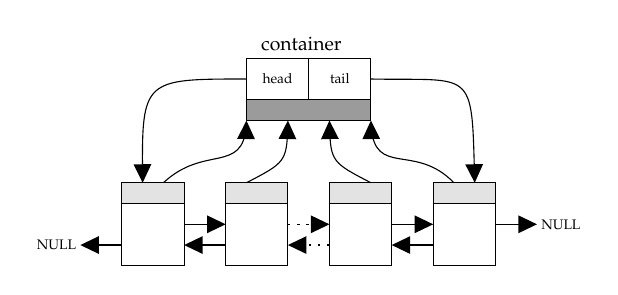
\begin{tikzpicture}[x=0.75pt,y=0.75pt,yscale=-1,xscale=1]
        \draw   (200,110) -- (230,110) -- (230,150) -- (200,150) -- cycle ;
        \draw    (230,130) -- (247,130) ;
        \draw [shift={(250,130)}, rotate = 180] [fill={rgb, 255:red, 0; green, 0; blue, 0 }  ][line width=0.08]  [draw opacity=0] (8.93,-4.29) -- (0,0) -- (8.93,4.29) -- cycle    ;
        \draw    (200,140) -- (183,140) ;
        \draw [shift={(180,140)}, rotate = 360] [fill={rgb, 255:red, 0; green, 0; blue, 0 }  ][line width=0.08]  [draw opacity=0] (8.93,-4.29) -- (0,0) -- (8.93,4.29) -- cycle    ;
        \draw   (250,110) -- (280,110) -- (280,150) -- (250,150) -- cycle ;
        \draw  [dash pattern={on 0.84pt off 2.51pt}]  (280,130) -- (297,130) ;
        \draw [shift={(300,130)}, rotate = 180] [fill={rgb, 255:red, 0; green, 0; blue, 0 }  ][line width=0.08]  [draw opacity=0] (8.93,-4.29) -- (0,0) -- (8.93,4.29) -- cycle    ;
        \draw    (250,140) -- (233,140) ;
        \draw [shift={(230,140)}, rotate = 360] [fill={rgb, 255:red, 0; green, 0; blue, 0 }  ][line width=0.08]  [draw opacity=0] (8.93,-4.29) -- (0,0) -- (8.93,4.29) -- cycle    ;
        \draw   (300,110) -- (330,110) -- (330,150) -- (300,150) -- cycle ;
        \draw    (330,130) -- (347,130) ;
        \draw [shift={(350,130)}, rotate = 180] [fill={rgb, 255:red, 0; green, 0; blue, 0 }  ][line width=0.08]  [draw opacity=0] (8.93,-4.29) -- (0,0) -- (8.93,4.29) -- cycle    ;
        \draw  [dash pattern={on 0.84pt off 2.51pt}]  (300,140) -- (283,140) ;
        \draw [shift={(280,140)}, rotate = 360] [fill={rgb, 255:red, 0; green, 0; blue, 0 }  ][line width=0.08]  [draw opacity=0] (8.93,-4.29) -- (0,0) -- (8.93,4.29) -- cycle    ;
        \draw   (350,110) -- (380,110) -- (380,150) -- (350,150) -- cycle ;
        \draw    (380,130) -- (397,130) ;
        \draw [shift={(400,130)}, rotate = 180] [fill={rgb, 255:red, 0; green, 0; blue, 0 }  ][line width=0.08]  [draw opacity=0] (8.93,-4.29) -- (0,0) -- (8.93,4.29) -- cycle    ;
        \draw    (350,140) -- (333,140) ;
        \draw [shift={(330,140)}, rotate = 360] [fill={rgb, 255:red, 0; green, 0; blue, 0 }  ][line width=0.08]  [draw opacity=0] (8.93,-4.29) -- (0,0) -- (8.93,4.29) -- cycle    ;
        \draw   (260,50) -- (290,50) -- (290,70) -- (260,70) -- cycle ;
        \draw    (320,60) .. controls (369.74,60.99) and (368.55,54.07) .. (369.93,107.52) ;
        \draw [shift={(370,110)}, rotate = 268.47] [fill={rgb, 255:red, 0; green, 0; blue, 0 }  ][line width=0.08]  [draw opacity=0] (8.93,-4.29) -- (0,0) -- (8.93,4.29) -- cycle    ;
        \draw    (260,60) .. controls (210.51,60) and (209.52,60) .. (209.97,107.06) ;
        \draw [shift={(210,110)}, rotate = 269.43] [fill={rgb, 255:red, 0; green, 0; blue, 0 }  ][line width=0.08]  [draw opacity=0] (8.93,-4.29) -- (0,0) -- (8.93,4.29) -- cycle    ;
        \draw   (290,50) -- (320,50) -- (320,70) -- (290,70) -- cycle ;
        \draw  [fill={rgb, 255:red, 155; green, 155; blue, 155 }  ,fill opacity=1 ] (260,70) -- (320,70) -- (320,80) -- (260,80) -- cycle ;
        \draw    (220,110) .. controls (239.78,91.53) and (258.17,105.78) .. (259.88,82.67) ;
        \draw [shift={(260,80)}, rotate = 451.07] [fill={rgb, 255:red, 0; green, 0; blue, 0 }  ][line width=0.08]  [draw opacity=0] (8.93,-4.29) -- (0,0) -- (8.93,4.29) -- cycle    ;
        \draw    (260,110) .. controls (278.52,100.36) and (279.45,99.88) .. (279.93,82.83) ;
        \draw [shift={(280,80)}, rotate = 451.44] [fill={rgb, 255:red, 0; green, 0; blue, 0 }  ][line width=0.08]  [draw opacity=0] (8.93,-4.29) -- (0,0) -- (8.93,4.29) -- cycle    ;
        \draw    (320,110) .. controls (301.47,100.36) and (300.55,99.88) .. (300.07,82.83) ;
        \draw [shift={(300,80)}, rotate = 448.56] [fill={rgb, 255:red, 0; green, 0; blue, 0 }  ][line width=0.08]  [draw opacity=0] (8.93,-4.29) -- (0,0) -- (8.93,4.29) -- cycle    ;
        \draw    (360,110) .. controls (341.18,90.56) and (321.9,107.58) .. (320.12,82.86) ;
        \draw [shift={(320,80)}, rotate = 449.01] [fill={rgb, 255:red, 0; green, 0; blue, 0 }  ][line width=0.08]  [draw opacity=0] (8.93,-4.29) -- (0,0) -- (8.93,4.29) -- cycle    ;
        \draw  [fill={rgb, 255:red, 210; green, 210; blue, 210 }  ,fill opacity=0.62 ] (200,110) -- (230,110) -- (230,120) -- (200,120) -- cycle ;
        \draw  [fill={rgb, 255:red, 210; green, 210; blue, 210 }  ,fill opacity=0.62 ] (250,110) -- (280,110) -- (280,120) -- (250,120) -- cycle ;
        \draw  [fill={rgb, 255:red, 210; green, 210; blue, 210 }  ,fill opacity=0.62 ] (300,110) -- (330,110) -- (330,120) -- (300,120) -- cycle ;
        \draw  [fill={rgb, 255:red, 210; green, 210; blue, 210 }  ,fill opacity=0.62 ] (350,110) -- (380,110) -- (380,120) -- (350,120) -- cycle ;
        \draw (275,60) node  [font=\tiny] [align=left] {\lstinline{head}};
        \draw (305,60) node  [font=\tiny] [align=left] {\lstinline{tail}};
        \draw (286.5,43) node  [font=\scriptsize] [align=left] {container};
        \draw (168.5,140) node  [font=\tiny] [align=left] {\lstinline{NULL}};
        \draw (411.5,130) node  [font=\tiny] [align=left] {\lstinline{NULL}};
    \end{tikzpicture}
    \caption{Doubly-linked list implementation}
    \label{fig:qlistsfigure}
\end{figure}

Nodes should be an user-defined data structure of any number of members, however, they must be specially defined to be compatible with the provided APIs. All the user-defined nodes must have the \lstinline{qNode_MinimalFields} definition on top of the structure. An example is shown below: \\

\begin{lstlisting}[style=CStyle]
typedef struct{
    qNode_MinimalFields; /*< required for lists*/
    int a;
    int b;
    float y;
}userdata_t;
\end{lstlisting}

With this special type definition on all custom data, the application writer can take advantage of this powerful data structure. The following APIs are provided for lists management:

\noindent\hrulefill


\begin{lstlisting}[style=CStyle]
void qList_Initialize( qList_t * const list )
\end{lstlisting}

Must be called before a list is used.  This initializes all the members of the 
list object. \index{\lstinline{qList_Initialize}}

\subsubsection*{Parameters:}
\begin{itemize}
    \item \lstinline{list} : Pointer to the list being initialised. 
\end{itemize}

\noindent\hrulefill

\begin{lstlisting}[style=CStyle]
qBool_t qList_Insert( qList_t *const list, void * const node, 
                      const qList_Position_t position ){
\end{lstlisting}

Insert an item into the list. \index{\lstinline{qList_Insert}}

\subsubsection*{Parameters:}
\begin{itemize}
    \item \lstinline{list} : Pointer to the list. 
    \item \lstinline{node} : A pointer to the node to be inserted.
    \item \lstinline{position} : The position where the node will be inserted. Could be \lstinline{qList_AtFront}, \lstinline{qList_AtBack} or any other index number where the node will be inserted after.
    
    \textit{Note}: If the index exceeds the size of the list, the node will be inserted at the back.
    
    \textit{Note}: If the list is empty, the node will be inserted as the first item.
\end{itemize}

\subsubsection*{Return value:}
\lstinline{qTrue} if the item was successfully added to the list, otherwise returns \lstinline{qFalse}. 

\noindent\hrulefill

\begin{lstlisting}[style=CStyle]
void* qList_Remove( qList_t * const list, void * const node, 
                    const qList_Position_t position )
\end{lstlisting}

Remove an item from the list. \index{\lstinline{qList_Remove}}

\subsubsection*{Parameters:}
\begin{itemize}
    \item \lstinline{list} : Pointer to the list. 
    \item \lstinline{node} : A pointer to the node to be deleted (to ignore pass \lstinline{NULL} ).
    \item \lstinline{position} : The position of the node that will be deleted. Could be \lstinline{qList_AtFront}, \lstinline{qList_AtBack} or any other index number.
    
    \textit{Note}: If the \lstinline{node} argument is supplied, the removal will be only effective if the data is member of the list. If ignored or the data is not a member of the list, this function will use the \lstinline{position} instead as index for removal.
    
    \textit{Note}: If the index exceeds the size of the list, the last node  will be removed.
\end{itemize}

\subsubsection*{Return value:}
A pointer to the removed node. \lstinline{NULL} if removal can be performed.

\noindent\hrulefill

\begin{lstlisting}[style=CStyle]
qBool_t qList_IsMember( const qList_t *const list, const void *const node )
\end{lstlisting}

Check if the node is member of the list. \index{\lstinline{qList_IsMember}}

\subsubsection*{Parameters:}
\begin{itemize}
    \item \lstinline{list} : Pointer to the list. 
    \item \lstinline{node} : A pointer to the node .
\end{itemize}

\subsubsection*{Return value:}
\lstinline{qTrue} if the node belongs to the list, \lstinline{qFalse} if it is not.

\noindent\hrulefill

\begin{lstlisting}[style=CStyle]
void* qList_GetFront( const qList_t *const list ){
\end{lstlisting}

Get a pointer to the front item of the list. \index{\lstinline{qList_GetFront}}

\subsubsection*{Parameters:}
\begin{itemize}
    \item \lstinline{list} : Pointer to the list. 
\end{itemize}

\subsubsection*{Return value:}
A pointer to the front node. \lstinline{NULL} if the list is empty.

\noindent\hrulefill

\begin{lstlisting}[style=CStyle]
void* qList_GetBack( const qList_t *const list )
\end{lstlisting}

Get a pointer to the back item of the list. \index{\lstinline{qList_GetBack}}

\subsubsection*{Parameters:}
\begin{itemize}
    \item \lstinline{list} : Pointer to the list. 
\end{itemize}

\subsubsection*{Return value:}
A pointer to the front node. \lstinline{NULL} if the list is empty.


\noindent\hrulefill

\begin{lstlisting}[style=CStyle]
qBool_t qList_IsEmpty( const qList_t * const list )
\end{lstlisting}

Check if the list is empty. \index{\lstinline{qList_IsEmpty}}

\subsubsection*{Parameters:}
\begin{itemize}
    \item \lstinline{list} : Pointer to the list. 
\end{itemize}

\subsubsection*{Return value:}
\lstinline{qTrue} if the list is empty, \lstinline{qFalse} if it is not.


\noindent\hrulefill

\begin{lstlisting}[style=CStyle]
size_t qList_Length( const qList_t * const list )
\end{lstlisting}

Get the number of items inside the list. \index{\lstinline{qList_Length}}

\subsubsection*{Parameters:}
\begin{itemize}
    \item \lstinline{list} : Pointer to the list. 
\end{itemize}

\subsubsection*{Return value:}
The number of items of the list. 

\noindent\hrulefill

\begin{lstlisting}[style=CStyle]
qBool_t qList_Move( qList_t *const destination, qList_t *const source, 
                    const qList_Position_t position )
\end{lstlisting} \index{\lstinline{qList_Move}}

Moves(or merge) the entire list pointed by \lstinline{source} to the list pointed by \lstinline{destination} at location specified by \lstinline{position}. 
After the move operation, this function leaves empty the list pointed by \lstinline{source}.

\subsubsection*{Parameters:}
\begin{itemize}
    \item \lstinline{destination} : Pointer to the list where the \lstinline{source} nodes are to be moved. 
    \item \lstinline{source} : Pointer to the source list to be moved.
    \item \lstinline{position} : The position where \lstinline{source} list will be inserted. Could be \lstinline{qList_AtFront}, \lstinline{qList_AtBack} or any other index number where the list will be inserted after.
\end{itemize}

\subsubsection*{Return value:}
\lstinline{qTrue} if the move operation is performed successfully, otherwise  returns \lstinline{qFalse}.  

\noindent\hrulefill

\begin{lstlisting}[style=CStyle]
qBool_t qList_ForEach( qList_t *const list, qList_NodeFcn_t Fcn, 
                       void *arg, qList_Direction_t dir, void *NodeOffset )
\end{lstlisting} \index{\lstinline{qList_ForEach}}

Operate on each element of the list.

\subsubsection*{Parameters:}
\begin{itemize}
    \item \lstinline{list} : Pointer to the list.
    \item \lstinline{Fcn} : The function to perform over the node. 
                            
                            Should have this prototype:
                            
                            \lstinline{ qBool_t Function( void* Node, void *arg, qList_WalkStage_t stage ) }
                            
                            where the \lstinline{stage} argument indicates the loop progress and should be checked by the application writer to perform the specific operations over the list. This variable can take the following values:
                            
                            \begin{itemize}
                                \item \lstinline{QLIST_WALKINIT} : When the loop is about to start. In this case, A \lstinline{NULL} value will be passed in the node pointer.
                                \item \lstinline{QLIST_WALKTHROUGH} : When the loop is traversing the list.
                                \item \lstinline{QLIST_WALKEND} :  When the loop has finished. In this case, A \lstinline{NULL} value will be passed in the node pointer
                            \end{itemize}
                            
                            By default, \lstinline{Function} should return \lstinline{qFalse}. If a \lstinline{qTrue} value is returned, the walk through loop will be terminated.
    \item \lstinline{arg} : Argument passed to \lstinline{Fcn}.
    \item \lstinline{dir} : Use one of the following options:
                            \begin{itemize}
                                \item \lstinline{QLIST_FORWARD} : to walk through the list forwards.
                                \item \lstinline{QLIST_BACKWARD} to walk through the list backwards.
                            \end{itemize}
    \item \lstinline{NodeOffset} : If available, the list walk through will start from this node.  
                   To ignore, pass \lstinline{NULL}.
\end{itemize}

\subsubsection*{Return value:}
\lstinline{qTrue} if the walk through was early terminated, otherwise returns \lstinline{qFalse}.

\noindent\hrulefill

\begin{lstlisting}[style=CStyle]
qBool_t qList_Sort( qList_t * const list, 
                    qBool_t (*CompareFcn)(const void *n1, const void *n2) ) 
\end{lstlisting} \index{\lstinline{qList_Sort}}

Sort the double linked list using the \lstinline{CompareFcn} function to 
determine the order.
The sorting algorithm used by this function compares pairs of adjacent nodes by calling the specified \lstinline{CompareFcn} function with pointers to them as arguments. The sort is performed only modifying node's links without data swapping, improving performance if nodes have a large storage.

\textit{Note:} The function modifies the content of the list by reordering its 
elements as defined by \lstinline{CompareFcn}.

\subsubsection*{Parameters:}
\begin{itemize}
    \item \lstinline{list} : Pointer to the list. 
    \item \lstinline{CompareFcn} : Pointer to a function that compares two nodes.
                    This function is called repeatedly by \lstinline{qList_Sort} to compare two nodes. It shall follow the following prototype:
                    \lstinline{qBool_t (*CompareFcn)(void *node1, void *node2)}
                    
                    Taking two pointers as arguments (both converted to (\lstinline{const void*}). The function defines the order of the elements by returning a Boolean data, where a \lstinline{qTrue} value indicates that element pointed by \lstinline{node1} goes after the element pointed to by \lstinline{node2}
\end{itemize}

\subsubsection*{Return value:}
\lstinline{qTrue} if at least one reordering is performed over the list. 


\noindent\hrulefill

\begin{lstlisting}[style=CStyle]
qBool_t qList_IteratorSet( qList_Iterator_t *iterator, qList_t *const list, 
                           void *NodeOffset, qList_Direction_t dir )
\end{lstlisting} \index{\lstinline{qList_IteratorSet}}

Setup an instance of the given iterator to traverse the list.

\subsubsection*{Parameters:}
\begin{itemize}
    \item \lstinline{iterator} : Pointer to the iterator instance. 
    \item \lstinline{list} : Pointer to the list.
    \item \lstinline{NodeOffset} : The start offset-node. To ignore, pass \lstinline{NULL}.
    \item \lstinline{dir} : Use one of the following options:
        \begin{itemize}
            \item \lstinline{QLIST_FORWARD} : to go in forward direction.
            \item \lstinline{QLIST_BACKWARD} : to go in backward direction.
        \end{itemize}
\end{itemize}

\subsubsection*{Return value:}
\lstinline{qTrue} on success. Otherwise returns \lstinline{qFalse}. 

\noindent\hrulefill

\begin{lstlisting}[style=CStyle]
void* qList_IteratorGetNext( qList_Iterator_t *iterator )
\end{lstlisting} \index{\lstinline{qList_IteratorGetNext}}

Get the current node available in the iterator. After invoked, iterator will be updated to the next node.

\subsubsection*{Parameters:}
\begin{itemize}
    \item \lstinline{iterator} : Pointer to the iterator instance. 
\end{itemize}

\subsubsection*{Return value:}
Return the next node or \lstinline{NULL} when no more nodes remain in the list. 

\noindent\hrulefill

\begin{lstlisting}[style=CStyle]
qBool_t qList_Swap( void *node1, void *node2 )
\end{lstlisting} \index{\lstinline{qList_Swap}}

Swap two nodes that belongs to the same list by changing its own links.

Note: The container list will be updated if any node is part of the boundaries.

\subsubsection*{Parameters:}
\begin{itemize}
    \item \lstinline{node1} : Pointer to the first node.
    \item \lstinline{node2} : Pointer to the second node.
\end{itemize}

\subsubsection*{Return value:}
\lstinline{qTrue} if the swap operation is performed. Otherwise returns \lstinline{qFalse}.


\subsection{Response handler}

\begin{lstlisting}[style=CStyle]
void qResponse_Setup( qResponse_t * const obj, char *xLocBuff, 
                      size_t nMax )
\end{lstlisting}

Initialize the instance of the response handler object. \index{\lstinline{qResponse_Setup}}

\subsubsection*{Parameters:}
\begin{itemize}
    \item \lstinline{obj} : A pointer to the response handler object
    \item \lstinline{xLocBuff} : A pointer to the memory block where the desired response will remain.
    \item \lstinline{nMax} : The size of memory block pointed by \lstinline{xLocBuff}
\end{itemize}

\noindent\hrulefill

\begin{lstlisting}[style=CStyle]
void qResponse_Reset( qResponse_t * const obj )
\end{lstlisting}

Reset the response handler. \index{\lstinline{qResponse_Reset}}

\subsubsection*{Parameters:}
\begin{itemize}
    \item \lstinline{obj} : A pointer to the response handler object
\end{itemize}

\noindent\hrulefill

\begin{lstlisting}[style=CStyle]
qBool_t qResponse_Received( qResponse_t * const obj, 
                            const char *Pattern, size_t n )
\end{lstlisting}

Non-blocking response check. \index{\lstinline{qResponse_Received}}

\subsubsection*{Parameters:}
\begin{itemize}
    \item \lstinline{obj} : A pointer to the response handler object.
    \item \lstinline{Pattern} : The data to be checked in the receiver ISR
    \item \lstinline{n} : The length of the data pointer by \lstinline{Pattern} . If \lstinline{Pattern} its string, set \lstinline{n} to zero(0) to auto-compute the length.
\end{itemize}

\subsubsection*{Return value:}
\lstinline{qTrue} if there is a response acknowledge, otherwise returns \lstinline{qFalse}.

\noindent\hrulefill

\begin{lstlisting}[style=CStyle]
qBool_t qResponse_ReceivedWithTimeout( qResponse_t * const obj, 
                                       const char *Pattern, 
                                       size_t n, qTime_t t )
\end{lstlisting}

Non-blocking response check with timeout. \index{\lstinline{qResponse_ReceivedWithTimeout}}

\subsubsection*{Parameters:}
\begin{itemize}
    \item \lstinline{obj} : A pointer to the response handler object.
    \item \lstinline{Pattern} : The data to be checked in the receiver ISR
    \item \lstinline{n} : The length of the data pointer by \lstinline{Pattern} . If \lstinline{Pattern} its string, set \lstinline{n} to zero(0) to auto-compute the length.
    \item \lstinline{obj} : The timeout value in seconds.
\end{itemize}

\subsubsection*{Return value:}
\lstinline{qTrue} if there is a response acknowledge and \lstinline{qTimeoutReached} if timeout expires,  otherwise returns \lstinline{qFalse}.

\noindent\hrulefill

\begin{lstlisting}[style=CStyle]
qBool_t qResponse_ISRHandler( qResponse_t * const obj, 
                              const char rxchar )
\end{lstlisting}

ISR receiver for the response handler. \index{\lstinline{qResponse_ISRHandler}}

\subsubsection*{Parameters:}
\begin{itemize}
    \item \lstinline{obj} : A pointer to the response handler object.
    \item \lstinline{rxchar} : The byte-data from the receiver.
\end{itemize}

\subsubsection*{Return value:}
\lstinline{qTrue} when the response handler object match the request from \lstinline{qResponse_Received()}.

\subsection{Miscellaneous}

\begin{lstlisting}[style=CStyle]
qTime_t qClock_Convert2Time( const qClock_t t )
\end{lstlisting}

Convert the specified input time(epochs) to time(seconds). \index{\lstinline{qClock_Convert2Time}}

\subsubsection*{Parameters:}
\begin{itemize}
    \item \lstinline{t} : The time in epochs
\end{itemize}

\subsubsection*{Return value:}
Time \lstinline{t} in seconds.
 
\noindent\hrulefill

\begin{lstlisting}[style=CStyle]
qClock_t qClock_Convert2Clock( const qTime_t t )
\end{lstlisting}

Convert the specified input time(seconds) to time(epochs). \index{\lstinline{qClock_Convert2Clock}}

\subsubsection*{Parameters:}
\begin{itemize}
    \item \lstinline{t} : The time in seconds
\end{itemize}

\subsubsection*{Return value:}
 Time \lstinline{t} in epochs.

\noindent\hrulefill

\begin{lstlisting}[style=CStyle]
void qIOUtil_SwapBytes( void *data, size_t n )
\end{lstlisting}

Invert the endianess for \lstinline{n} bytes of the specified memory location. \index{\lstinline{qIOUtil_SwapBytes}}

\subsubsection*{Parameters:}
\begin{itemize}
    \item \lstinline{data} : A pointer to block of data.
    \item \lstinline{n} : Number of bytes to swap.
\end{itemize}

\noindent\hrulefill

\begin{lstlisting}[style=CStyle]
qBool_t qIOUtil_CheckEndianness( void )
\end{lstlisting}

Check the system endianess. \index{\lstinline{qIOUtil_CheckEndianness}}

\subsubsection*{Return value:}
\lstinline{qTrue} if little-endian, otherwise returns \lstinline{qFalse}.

\noindent\hrulefill

\begin{lstlisting}[style=CStyle]
void qIOUtil_OutputRaw( qPutChar_t fcn, void* storagep, void *data, 
                        size_t n, qBool_t AIP )
void qIOUtil_InputRaw( qGetChar_t fcn, void* storagep, void *data, 
                       size_t n, qBool_t AIP )
\end{lstlisting}

Wrapper methods to write(\lstinline{qIOUtil_OutputRaw}) \index{\lstinline{qIOUtil_OutputRaw}} or read(\lstinline{qIOUtil_InputRaw}) \index{\lstinline{qIOUtil_InputRaw}} \lstinline{n} RAW data through \lstinline{fcn}.

\subsubsection*{Parameters:}
\begin{itemize}
    \item \lstinline{fcn} : The basic output or input byte function.
    \item \lstinline{storagep} : The storage pointer passed to \lstinline{fcn}.
    \item \lstinline{data}: The data to be written or readed.
    \item \lstinline{n} : Number of bytes to be writte or readed.
    \item \lstinline{AIP} : Pass \lstinline{qTrue} to auto-increment the storage-pointer.
\end{itemize}

\noindent\hrulefill

\begin{lstlisting}[style=CStyle]
void qIOUtil_OutputString( qPutChar_t fcn, void* storagep, const char *s, 
                           qBool_t AIP )
\end{lstlisting}

Wrapper method to write a string through \lstinline{fcn}. \index{\lstinline{qIOUtil_OutputString}}

\subsubsection*{Parameters:}
\begin{itemize}
    \item \lstinline{fcn} : The basic output byte function.
    \item \lstinline{storagep} : The storage pointer passed to \lstinline{fcn}.
    \item \lstinline{s} : The string to be written.
    \item \lstinline{AIP} : Pass \lstinline{qTrue} to auto-increment the storage-pointer.
\end{itemize}

\noindent\hrulefill

\begin{lstlisting}[style=CStyle]
void qIOUtil_U32toX( qUINT32_t value, char *str, int8_t n )
\end{lstlisting}

Converts an unsigned integer value to a null-terminated string using the 16 base and stores the result in the array given by \lstinline{str} parameter. \lstinline{str} should be an array long enough to contain any possible value. \index{\lstinline{qIOUtil_U32toX}}

\subsubsection*{Parameters:}
\begin{itemize}
    \item \lstinline{value} : Value to be converted to string.
    \item \lstinline{str} : Array in memory where to store the resulting null-terminated string.
    \item \lstinline{n} : The number of chars used to represent the value in \lstinline{str}. 
\end{itemize}


\noindent\hrulefill

\begin{lstlisting}[style=CStyle]
qUINT32_t qIOUtil_XtoU32( const char *s )
\end{lstlisting}

Converts the input string \lstinline{s} consisting of hexadecimal digits into an unsigned 
integer value. The input parameter \lstinline{s} should consist exclusively of hexadecimal 
digits, with optional whitespaces. The string will be processed one character at
a time, until the function reaches a character which it doesn't recognize
(including a null character). \index{\lstinline{qIOUtil_XtoU32}}
 
\subsubsection*{Parameters:}
\begin{itemize}
    \item \lstinline{s} : The hex string to be converted.
\end{itemize}

\subsubsection*{Return value:}
The numeric value in \lstinline{qUINT32_t}.


\noindent\hrulefill

\begin{lstlisting}[style=CStyle]
qFloat64_t qIOUtil_AtoF( const char *s )
\end{lstlisting}

Parses the C string \lstinline{s}, interpreting its content as a floating point number and 
returns its value as a double. The function first discards as many whitespace 
characters (as in \lstinline{isspace}) as necessary until the first non-whitespace character is found. Then, starting from this character, takes as many characters as possible that are valid following a syntax resembling that of floating point literals, and 
interprets them as a numerical value. The rest of the string after the last valid 
character is ignored and has no effect on the behavior of this function. \index{\lstinline{qIOUtil_AtoF}}

\subsubsection*{Parameters:}
\begin{itemize}
    \item \lstinline{s} : The string beginning with the representation of a floating-point number.
\end{itemize}

\subsubsection*{Return value:}
On success, the function returns the converted floating point number as  a double value. \\
If no valid conversion could be performed, the function returns zero (0.0). \\
If the converted value would be out of the range of representable values by a \lstinline{double}, it causes undefined behavior.


\noindent\hrulefill

\begin{lstlisting}[style=CStyle]
int qIOUtil_AtoI( const char *s )
\end{lstlisting}

Parses the C-string \lstinline{s} interpreting its content as an integral number, which is returned as a value of type \lstinline{int}. The function first discards as many whitespace characters (as in \lstinline{isspace}) as necessary until the first non-whitespace character is found. Then, starting from this character, takes an optional initial plus or minus sign followed by as many base-10 digits as possible, and interprets them as a numerical value. \index{\lstinline{qIOUtil_AtoI}}
The string can contain additional characters after those that form the integral number, which are ignored and have no effect on the behavior of this function. If the first sequence of non-whitespace characters in \lstinline{s} is not a valid integral number, or if no such sequence exists because either \lstinline{s} is empty or it contains only whitespace characters, no conversion is performed and zero is returned.

\subsubsection*{Parameters:}
\begin{itemize}
    \item \lstinline{s} : The string beginning with the representation of a integer number.

\end{itemize}

\subsubsection*{Return value:}
On success, the function returns the converted integral number as an int value. \\
If the converted value would be out of the range of representable values by an \lstinline{int}, it causes undefined behavior.


\noindent\hrulefill

\begin{lstlisting}[style=CStyle]
char* qIOUtil_UtoA( qUINT32_t num, char* str, qUINT8_t base )
\end{lstlisting}

Converts an unsigned value to a null-terminated string using the specified base and stores the result in the array given by \lstinline{str} parameter. \lstinline{str} should be an array long enough to contain any possible value: \lstinline{(sizeof(int)*8+1)} for radix=2, i.e. 17 bytes in 16-bits platforms and 33 in 32-bits platforms. \index{\lstinline{qIOUtil_UtoA}}

\subsubsection*{Parameters:}
\begin{itemize}
    \item \lstinline{num} : Value to be converted to a string.
    \item \lstinline{str} : Array in memory where to store the resulting null-terminated string.
    \item \lstinline{base} : Numerical base used to represent the value as a string, between 2 and 36, where 10 means decimal base, 16 hexadecimal, 8 octal, and 2 binary.
\end{itemize}

\subsubsection*{Return value:}
A pointer to the resulting null-terminated string, same as parameter \lstinline{str}.


\noindent\hrulefill

\begin{lstlisting}[style=CStyle]
char* qIOUtil_ItoA( qINT32_t  num, char* str, qUINT8_t base )
\end{lstlisting}

Converts an integer value to a null-terminated string using the specified \lstinline{base} and stores the result in the array given by \lstinline{str} parameter. If \lstinline{base} is 10 and value is negative, the resulting string is preceded with a minus sign (-). With any other base, value is always considered unsigned. \index{\lstinline{qIOUtil_ItoA}}

\lstinline{str} should be an array long enough to contain any possible value: \lstinline{(sizeof(int)*8+1)} for radix=2, i.e. 17 bytes in 16-bits platforms and 33 in 32-bits platforms.

\subsubsection*{Parameters:}
\begin{itemize}
    \item \lstinline{num} : Value to be converted to a string.
    \item \lstinline{str} : Array in memory where to store the resulting null-terminated string.
    \item \lstinline{base} : Numerical base used to represent the value as a string, between 2 and 36, where 10 means decimal base, 16 hexadecimal, 8 octal, and 2 binary.
\end{itemize}

\subsubsection*{Return value:}
A pointer to the resulting null-terminated string, same as parameter \lstinline{str}.


\noindent\hrulefill

\begin{lstlisting}[style=CStyle]
char* qIOUtil_FtoA( qFloat32_t f, char *str, qUINT8_t precision )
\end{lstlisting}

Converts a float value to a formatted string. \index{\lstinline{qIOUtil_FtoA}}

\subsubsection*{Parameters:}
\begin{itemize}
    \item \lstinline{f} : Value to be converted to a string.
    \item \lstinline{str} : Array in memory where to store the resulting null-terminated string.
    \item \lstinline{precision} : Desired number of significant fractional digits in the string. (The max allowed precision is \lstinline{MAX_FTOA_PRECISION=10})
\end{itemize}

\subsubsection*{Return value:}
A pointer to the resulting null-terminated string, same as parameter \lstinline{str}.


\noindent\hrulefill

\begin{lstlisting}[style=CStyle]
char* qIOUtil_BtoA( qBool_t num, char *str )
\end{lstlisting}

Converts a boolean value to a null-terminated string. Input is considered true
with any value different to zero (0). \index{\lstinline{qIOUtil_BtoA}}
\lstinline{str} should be an array long enough to contain the output

\subsubsection*{Parameters:}
\begin{itemize}
    \item \lstinline{num} : Value to be converted to a string.
    \item \lstinline{str} : Array in memory where to store the resulting null-terminated string.
\end{itemize}

\subsubsection*{Return value:}
A pointer to the resulting null-terminated string, same as parameter \lstinline{str}.



\noindent\hrulefill

\begin{lstlisting}[style=CStyle]
qBool_t qIOUtil_IsNan( qFloat32_t f )
\end{lstlisting}

Determines if the given floating point number \lstinline{f} is a not-a-number(\lstinline{NaN}) value. \index{\lstinline{qIOUtil_IsNan}}

\subsubsection*{Parameters:}
\begin{itemize}
    \item \lstinline{f} : Floating point value(32bits).
\end{itemize}

\subsubsection*{Return value:}
\lstinline{qTrue} if input is \lstinline{NaN}, otherwise \lstinline{qFalse}.


\noindent\hrulefill

\begin{lstlisting}[style=CStyle]
qBool_t qIOUtil_IsInf( qFloat32_t f )
\end{lstlisting}

Determines if the given floating point number \lstinline{f} is positive or negative infinity. \index{\lstinline{qIOUtil_IsInf}}

\subsubsection*{Parameters:}
\begin{itemize}
    \item \lstinline{f} : Floating point value(32bits).
\end{itemize}

\subsubsection*{Return value:}
\lstinline{qTrue} is argument has an infinite value, otherwise \lstinline{qFalse}.

\subsection{Additional macros}

\lstinline{qFLM_BitsSet(Register, Bits)} : Sets (writes a 1 to) the bits indicated by the \lstinline{Bits} mask in the numeric variable \lstinline{Register}.

\noindent\hrulefill

\lstinline{qFLM_BitsClear(Register, Bits)} : Clears (writes a 0 to) the bits indicated by the \lstinline{Bits} mask in the numeric variable \lstinline{Register}.

\noindent\hrulefill

\lstinline{qFLM_BitSet(Register, Bit)} : Sets (writes a 1 to) the \lstinline{n-Bit} in the numeric variable \lstinline{Register}.

\noindent\hrulefill

\lstinline{qFLM_BitClear(Register, Bit)} : Clears (writes a 0 to) the \lstinline{n-Bit} in the numeric variable \lstinline{Register}.

\noindent\hrulefill

\lstinline{qFLM_BitRead(Register,Bit)} : Reads the \lstinline{n-Bit} of the numeric variable \lstinline{Register}.

\noindent\hrulefill

\lstinline{qFLM_BitToggle(Register,Bit)} : Invert the state of the \lstinline{n-Bit} in the numeric variable \lstinline{Register}.

\noindent\hrulefill

\lstinline{qFLM_BitWrite(Register, Bit, Value)} : Writes the \lstinline{Value} to the \lstinline{n-Bit} in the numeric variable \lstinline{Register}.

\noindent\hrulefill

\lstinline{qFLM_BitMakeByte(b7,b6,b5,b4,b3,b2,b1,b0)} : Merge the bits from the most significant bit \lstinline{b7} to the least significant bit \lstinline{b0} into a single byte.

\noindent\hrulefill

\lstinline{qFLM_ByteHighNibble(Register)} : Extracts the  high-order (leftmost) nibble of a byte.

\noindent\hrulefill

\lstinline{qFLM_ByteLowNibble(Register)} : Extracts the low-order (rightmost) nibble of a byte.

\noindent\hrulefill

\lstinline{qFLM_ByteMergeNibbles(H,L)} :  Merge the high(\lstinline{H}) and low(\lstinline{L}) nibbles into a single byte.

\noindent\hrulefill

\lstinline{qFLM_WordHighByte(Register)} : Extracts the high-order (leftmost) byte of a word.

\noindent\hrulefill

\lstinline{qFLM_WordLowByte(Register)} : Extracts the low-order (rightmost) byte of a word.

\noindent\hrulefill

\lstinline{qFLM_WordMergeBytes(H,L)} : Merge the high(\lstinline{H}) and low(\lstinline{L}) bytes into a single word.

\noindent\hrulefill

\lstinline{qFLM_DWordHighWord(Register)} : Extracts the high-order (leftmost) word of a Dword.

\noindent\hrulefill

\lstinline{qFLM_DWordLowWord(Register)} : Extracts the low-order (rightmost) word of a Dword.

\noindent\hrulefill

\lstinline{qFLM_DWordMergeWords(H,L) } : Merge the high(\lstinline{H}) and low(\lstinline{L}) words into a single DWord.

\noindent\hrulefill

\lstinline{qFLM_Clip(X, Max, Min)} :  Gives \lstinline{X} for \lstinline{Min<=X<=Max}, \lstinline{Min} for \lstinline{X<Min} and \lstinline{Max} for \lstinline{X>Max}.

\noindent\hrulefill

\lstinline{qFLM_ClipUpper(X, Max)} : Gives \lstinline{X} for \lstinline{X<=Max} and \lstinline{Max} for \lstinline{X>Max}.

\noindent\hrulefill

\lstinline{qFLM_ClipLower(X, Min)} : Gives \lstinline{X} for \lstinline{X>=Min} and \lstinline{Min} for \lstinline{X<Min}.

\noindent\hrulefill

\lstinline{qFLM_IsBetween(X, Low, High)} : Returns \lstinline{true} if the value in \lstinline{X} is between \lstinline{Low} and \lstinline{High}, otherwise returns \lstinline{false}.

\noindent\hrulefill

\lstinline{qFLM_Min(a,b)} : Returns the smaller of \lstinline{a} and \lstinline{b}.

\noindent\hrulefill

\lstinline{qFLM_Max(a,b)} :  Returns the greater of \lstinline{a} and \lstinline{b}.

\newpage

\bibliographystyle{unsrt}
\bibliography{references}

\printindex

\end{document}